\documentclass[a4paper,11pt,twoside]{tesis}

\usepackage[footnotesize]{caption}

\usepackage[spanish,english]{babel}
\usepackage[latin1]{inputenc}
\usepackage{etaremune}
\usepackage{hyperref}
\usepackage{dropcaps}
\usepackage{amsfonts,amssymb,amsmath}
\usepackage{latexsym}
\usepackage{makeidx}
\usepackage{epsfig}
\usepackage[mathscr]{eucal}
\usepackage{color}
%\usepackage{macrosangel}
\usepackage[all]{xy}
%\usepackage{macros}
%\usepackage{hyperref}
\usepackage{fancyhdr}
\usepackage{multirow}
\usepackage{cite}
\usepackage{soul}


%%%%%%% PAQUETES  ADICIONALES  EN LOS DOS ENTORNO MAC Y PC

%*******   NOTA:   TESIS.STY ha cambiado, he 

\usepackage{programs,keywords}
\usepackage{cancel,calc,underbr}

\usepackage{graphicx}
\usepackage{moreverb}
\usepackage{amssymb,amsmath,color,nicefrac,amsthm}
\usepackage{wasysym}
\usepackage{multicol}
%	\usepackage[latin1]{inputenc}
\usepackage{cancel}
\usepackage{array}
\usepackage[table]{xcolor}
\usepackage{latexsym}

\usepackage{mathrsfs}
%\usepackage[noline,tworuled,figure]{algorithm2e}
\usepackage{url}
\usepackage{pifont}% http://ctan.org/pkg/pifont
\newcommand{\cmark}{\ensuremath{\mathbf\square\!\!\!\!{\checkmark}}}%
\setlength{\leftmargin}{-0.007\textwidth}
\setlength{\textwidth}{1.015\textwidth}
\newcommand{\xmark}{{\ensuremath{\square\!\!\!\!{\times}}}}%
\usepackage[algo2e,ruled,vlined,algochapter,linesnumberedhidden]{algorithm2e}
\usepackage{color}
\newcounter{cpt}
\setcounter{cpt}{1}
\newcommand{\Pcpt}{P\thecpt.\stepcounter{cpt}}

%%%%% PAQUETE PARA COMENTARIOS Y ANOTACIONES

\usepackage{fixme}
\fxsetup{
    status=draft,
    author= Fernando, % Autor principal del documento
    layout= margin,
    theme=color,
    mode = multiuser % Lo configuramos para edici�n colaborativa
}
 %\fxuseenvlayout{colorsig}


 \FXRegisterAuthor{cr}{acr}{Carlos} % registro de autor para Carlos, con los prefijos de los comandos para comentarios y anotaciones
 \FXRegisterAuthor{me}{ame}{Manolo} % registro de autor para Manolo




%%%%%%%%%%%%%%%%%%%%%%%%%%%%%%%%%%%%%%%%%%%%%%%%%%%%%%%%%%%%%%%%%%%%%%%%%%%%%%%%
%%%%%   DEFINITIONS
%%%%%%%%%%%%%%%%%%%%%%%%%%%%%%%%%%%%%%%%%%%%%%%%%%%%%%%%%%%%%%%%%%%%%%%%%%%%%%%%

\newtheorem{theorem}{Teorema}[section]

\newenvironment{notation}
	{\par\smallskip\noindent\textsc{Notation}: }
	{\par\noindent}
\newtheorem{proposicion}[theorem]{Proposici�n}
\newtheorem{definicion}[theorem]{Definici�n}
\newtheorem{ejemplo}[theorem]{Ejemplo}
\newtheorem{corolario}[theorem]{Corolario}
\newtheorem{lema}[theorem]{Lema}
\newtheorem{remark}[theorem]{Nota}
\newtheorem{demostracion}{\textit Demostraci�n}

\def\I{\ensuremath{\mathrel{I}}}
%\bibliographystyle{PhDbiblio-url2} % Title is link if provided
\renewcommand{\bibname}{References} % changes the header; default: Bibliography

\newcommand{\rs}{\textit{sicumaRS}}
\newcommand{\rse}{\textit{sicumaRS} }
%\newcommand{\cierre}{\textit{$Cierre_{SLFD}$}}
%\newcommand{\cierree}{\textit{$Cierre_{SLFD}$} }

% =============== COMANDOS ================
\newcommand{\df}{$R = \langle U,F \rangle$ }
\newcommand{\uno}{$\mathbb{K}$1 }
\newcommand{\dos}{$\mathbb{K}$2 }
\newcommand{\slfd}{$SL_{FD}$}
\newcommand{\slfde}{$SL_{FD}$ }
\newcommand{\sst}{$SST$}
\newcommand{\sste}{$SST$ }
\newcommand{\ssk}{$SSK$} % cierre
\newcommand{\sske}{$SSK$ }
\newcommand{\sck}{$CK$} % cierreIJCM
\newcommand{\scke}{$SCK$ }

\newcommand{\smod}{$SST$}
\newcommand{\smode}{$SST$ }
%\newcommand{\cierre}{$SSK$}
%\newcommand{\cierree}{$SSK$ }
\newcommand{\cierreIJCM}{$SCK$}
\newcommand{\cierreIJCMe}{$SCK$ }
\newcommand{\cierre}{\ref{algoritmo:Cls}}
\newcommand{\cierree}{\ref{algoritmo:Cls} }

\newcommand{\QED}{\hfill {\qed}}
%==========================================



%----------------------
%    FORMATO DE PAGINA:
%----------------------

\setlength{\evensidemargin}{1cm} \setlength{\oddsidemargin}{2.5cm}
\setlength{\textwidth}{12.5cm} \setlength{\topmargin}{-0.25in}
\setlength{\textheight}{18cm}

\renewcommand{\baselinestretch}{1.15}

\pagestyle{plain}

%\renewcommand{\indexname}{Index}

%---------------------
%       PARA GRAFICOS:
%---------------------

\newdimen\unidad
\unidad = 1mm
\def\caja#1#2{\fbox{\begin{minipage}[t]{#1\unidad} #2 \end{minipage}}}





%-------------------------------------
%---------------------

%\newcounter{diag}
%\renewcommand\thediag{{\bf Diag}$_{\arabic{diag}}$}
%\newcommand\diagconta{\refstepcounter{diag}\thediag}
%\def\msup{\mbox{\rm Multi-sup}}
%\def\minf{\mbox{\rm Multi-inf}}

%\thispagestyle{empty} 
\pagestyle{headings} 
%%
%% OPCIONES DE FANCYHEADINGS
%%
%\fancyhf{}
%\fancyhead[LO]{\scshape \nouppercase\rightmark}
%\fancyhead[RE]{\scshape \nouppercase\leftmark}
%\fancyhead[RO,LE]{\thepage}
%\fancypagestyle{headings}{%
%  \fancyhf{}%
%  \renewcommand{\headrulewidth}{0pt}
%}
%%
\makeindex



\renewcommand{\theenumi}{\rm(\roman{enumi})}
\renewcommand{\labelenumi}{\theenumi}
\renewcommand{\labelitemi}{\scriptsize $\bullet$}


%\includeonly{Cap0-PreAlge17MayDEFI, Cap1-PreBases17MayDEFI} \pagestyle{headings}
%\includeonly{Cap2-idealOND1_20May02}
\begin{document}


\pagestyle{empty}


\frontmatter
\thispagestyle{empty}

PORTADA \ldots



\clearemptydoublepage

%\include{Portada}
%\clearemptydoublepage


\thispagestyle{empty}

 
\vspace*{3cm}

\begin{flushright}
\textit{A mi querida Aurora,}
\end{flushright}
 

\begin{flushright}
\textit{a mi padre y a mi madre,}
\end{flushright}

\begin{flushright}
\textit{a mi hermano,}
\end{flushright}
 
\begin{flushright}
\textit{por el apoyo y la confianza que\\
 siempre me hab�is demostrado.}
\end{flushright}
\clearemptydoublepage


\vspace*{3cm}

\begin{flushright}
\textit{En todo objetivo conseguido hay siempre una especial tristeza,\\ en el conocimiento de que una meta largamente deseada\\ se ha logrado al fin, y que la vida tiene entonces que ser\\ moldeada y encaminada en busca de nuevos fines.}
\end{flushright}

\begin{flushright}
\textit{\textit{La Ciudad y las Estrellas}}
\end{flushright}

\begin{flushright}
\textit{A. C. Clarke}
\end{flushright}

\clearemptydoublepage

\pagestyle{empty}


\setcounter{page}{1}

\selectlanguage{spanish}
\clearemptydoublepage


\chapter*{Agradecimientos}\label{agradecimientos_chapter}  
%\addcontentsline{toc}{chapter}{\protect{Agradecimientos}}
\thispagestyle{empty}
\markboth{Agradecimientos}{Agradecimientos}
Agradecimientos

dadsadsad

as
dasdas
d
sa
dsad



sd
as
dsa
d



adsasda



%\pagestyle{headings}
 

Texto \ldots

\clearemptydoublepage

%\selectlanguage{english}

\pagestyle{headings}



%===============================================================
%           Fin  Agradecimiento
%===============================================================



\tableofcontents 
\clearemptydoublepage \cleardoublepage

\selectlanguage{spanish}


%\selectlanguage{english}
\chapter*{Aportaciones}
\label{cap:aportaciones}
\addcontentsline{toc}{chapter}{\protect{Aportaciones}}

\markboth{Aportaciones}{Aportaciones}

A continuaci�n se expone una lista de los trabajos que han sido publicados como resultado de la investigaci�n llevada a cabo a lo largo de esta tesis doctoral. Estas publicaciones avalan el trabajo realizado poniendo de manifiesto tanto su inter�s como su validez cient�fica.\\

\begin{Large}
Revistas
\end{Large}

\begin{enumerate}
	\item Fernando Benito-Picazo, Pablo Cordero, Manuel Enciso, �ngel Mora. \textit{Minimal generators, an affordable approach by means of massive computation}. The Journal of Supercomputing, Springer, 2018. 
	
	DOI: 10.1007/s11227-018-2453-z.
	
Factor de impacto en J.C.R. 2016: 1,349. Posici�n 52 de 104 (Q2) en la categor�a: `Computer Science, Theory \& Methods'.
	\item Fernando Benito-Picazo, Manuel Enciso, Carlos Rossi, Antonio Guevara. \textit{Enhancing the conversational process by using a logical closure operator in phenotypes implications}. Mathematical Methods in the Applied Sciences, John Wiley \& Sons Ltd, 2017. 
	
	DOI: 10.1002/mma.4338.
	
Factor de impacto en J.C.R. 2016: 1,017. Posici�n 108 de 255 (Q2) en la categor�a: `Mathematics, Applied'.
	\item Fernando Benito-Picazo, Pablo Cordero, Manuel Enciso, �ngel Mora. \textit{Reducing the search space by closure and simplification paradigms. A parallel key finding method}. The Journal of Supercomputing, Springer, 2016. 
	
	DOI: 10.1007/s11227-016-1622-1.
	
Factor de impacto en J.C.R. 2016: 1,349. Posici�n 52 de 104 (Q2) en la categor�a: `Computer Science, Theory \& Methods'.
\end{enumerate}

\begin{Large}
Congresos
\end{Large}

\begin{itemize}
	\item Fernando Benito-Picazo, Pablo Cordero, Manuel Enciso, �ngel Mora. \textit{Closed sets enumeration: a logical approach}. Proceedings of the Seventeenth International Conference on Computational and Mathematical Methods in Science and Engineering, CMMSE, 2017. C�diz, Spain, July 4-8, pp. 287-292, ISBN: 978-84-617-8694-7.
	\item Fernando Benito-Picazo, Manuel Enciso, Carlos Rossi, Antonio Guevara. \textit{Conversational recommendation to avoid the cold-start problem}. Proceedings of the Sixteenth International Conference on Computational and Mathematical Methods in Science and Engineering, CMMSE, 2016. C�diz, Spain, July 4-8, pp. 184-190, ISBN: 978-84-608-6082-2.
	\item Fernando Benito-Picazo, Pablo Cordero, Manuel Enciso, �ngel Mora. \textit{Keys for the fusion of heterogeneous information}. Proceedings of the Fifteenth International Conference on Computational and Mathematical Methods in Science and Engineering, CMMSE, 2015. C�diz, Spain, July 6-10, pp. 201-211, ISBN: 978-84-617-2230-3.
	\item Fernando Benito-Picazo, Pablo Cordero, Manuel Enciso, �ngel Mora. \textit{Increasing the Efficiency of Minimal Key Enumeration Methods by Means of Parallelism}. Proceedings of the 9th International Conference on Software Engineering and Applications, ICSOFT-EA, Vienna, Austria, August 29-31, 2014, pp. 512-517.
	
	DOI: 10.5220/0005108205120517. 
\end{itemize}
\clearemptydoublepage


\pagestyle{empty}
\chapter*{Resumen}
\addcontentsline{toc}{chapter}{\protect{Resumen}}

\markboth{Resumen}{Resumen}

\pagestyle{headings}
 
Los sistemas de informaci�n est�n experimentando una gran expansi�n debido, en gran medida, al enorme crecimiento de la cantidad de informaci�n que se genera en la sociedad actual. Es por tanto un reto el investigar t�cnicas que permitan sacar partido y gestionar tales cantidades de informaci�n. En este marco, existen numerosos campos de conocimiento como pueden ser: sistemas inteligentes, big data \cite{Miao2014}, cloud computing, etc. Concretamente, esta tesis doctoral se sit�a en el �mbito del tratamiento de la informaci�n desde el punto de vista del an�lisis de conceptos formales (FCA), con la intenci�n de aplicarlo en �mbitos diferentes de la ingenier�a inform�tica como son las bases de datos y los sistemas de recomendaci�n.

FCA es una teor�a matem�tica y un m�todo para el an�lisis de datos en cuanto a sus relaciones y estructura. El cometido principal de FCA es definir un m�todo basado en las matem�ticas y la l�gica que corresponda al pensamiento conceptual del ser humano. Es una t�cnica con una s�lida base formal \cite{Ganter1997} que puede ser aplicable a un conjunto variado de disciplinas como pueden ser: data mining \cite{Stumme2002}, sistemas inteligentes, machine learning \cite{Mitchell1997}, web sem�ntica \cite{Wang2006}, desarrollo software, etc. FCA se ha establecido como una alternativa s�lida al proceso de la adquisici�n y tratamiento de la informaci�n para su posterior uso en aplicaciones usando t�cnicas de razonamiento autom�tico. M�s concretamente, se ha visto reconocido mediante un aumento muy significativo de aplicaciones en �reas muy diversas entre las que podemos destacar la biomedicina, turismo, educaci�n, web sem�ntica, desarrollo de software, biolog�a, redes sociales, etc. Gran parte de este creciente inter�s radica en disponer de un marco �nico en el que poder desarrollar de principio a fin el ciclo que nos lleva de la informaci�n al conocimiento y, sobre �l, poder realizar tareas de razonamiento autom�tico.

Hay diversas t�cnicas usadas con mucho �xito en tareas de miner�a de datos, clasificaci�n, etc. Pero una vez llevadas a cabo estas tareas, debemos hacer uso de otras �reas para trabajar con el conocimiento adquirido. Sin embargo, una gran diferencia entre gran parte de tales aproximaciones y FCA es que �sta �ltima busca recopilar todo el conocimiento existente en el sistema. As�, mientras en otras �reas el t�rmino aproximado es habitual, aqu� nos encontramos con un requerimiento importante en cuanto a la completitud sem�ntica. Evidentemente, este objetivo conlleva una gran complejidad y es natural que el sistema se vea representado por ret�culos de conceptos de gran tama�o o por sistemas de implicaciones igualmente grandes. Sin embargo, se ha hecho un gran esfuerzo �ltimamente en el desarrollo de t�cnicas y m�todos eficientes que han allanado el terreno en el marco del FCA cl�sico.

%Nuevas aplicaciones, como pueden ser los sistemas de comercio electr�nico \cite{Guo2014}, est�n demandando una mayor potencia expresiva que les permita una interacci�n m�s cercana para con el usuario final. As� por ejemplo, queremos poder agilizar un supuesto sistema de diagn�stico, de modo que a partir de una reducida informaci�n proporcionada por un paciente, seamos capaces de proponer un primer diagn�stico general; o bien, si buscamos hospedarnos en un hotel cercano a la celebraci�n de alg�n evento, haremos hincapi� en encontrar una buena ubicaci�n, mientras que la calidad que presenten servicios de ocio del hotel tendr� una menor importancia. Estos prop�sitos implican un desarrollo nuevo desde la extracci�n de implicaciones hasta las l�gicas que las manejan.

A partir de la informaci�n disponible, las relaciones l�gicas que se obtienen son aquellas que vengan confirmadas por nuestros contextos formales, que podemos considerar como tablas de datos que relacionan la informaci�n existente entre un conjuntos de objetos y un conjunto de atributos. Principalmente, existen dos formas b�sicas para representar el conocimiento extra�do de estas tablas: los ret�culos de conceptos y los conjuntos de implicaciones. 

Desde hace a�os, existen en la literatura estudios \cite{Kuznetsov2002} donde se han investigado y comparado diferentes algoritmos para obtener el ret�culo de conceptos a partir del conjunto de datos. La dificultad de utilizar ret�culos de conceptos se debe a que su tama�o puede alcanzar cotas que, en el peor de los casos, supongan un coste computacional muy elevado para los m�todos encargados de su construcci�n, lo cual constituye una limitaci�n en la aplicaci�n de FCA.

Por otro lado, las implicaciones pueden considerarse como reglas del tipo \textit{si-entonces}, que reflejan un concepto muy intuitivo: cuando se verifica una premisa, entonces se cumple una conclusi�n. Consecuentemente, en FCA podemos formalizarlo de la siguiente forma: dados $A$ y $B$ subconjuntos de atributos, diremos que se tiene la implicaci�n $A \rightarrow B$ si se verifica $A' \in B'$, es decir, todos los objetos que tienen cada atributo de $A$ tambi�n tienen cada atributo de $B$. Con esta definici�n, las implicaciones obedecen los Axiomas de Armstrong \cite{Armstrong74} (reflexivo, aumentativo y transitivo) comunes en las dependencias funcionales que se dan entre los atributos de una base de datos y considerados como el primer sistema de inferencia para dependencias funcionales completo. Trabajar con conjuntos de implicaciones nos permite aplicar t�cnicas autom�ticas basadas en la l�gica. Este hecho se alza como el objetivo principal de esta tesis doctoral, que principalmente consiste en aplicar mecanismos l�gicos sobre conjuntos de implicaciones que nos permitan desarrollar m�todos para realizar un tratamiento eficiente de la informaci�n.

La aproximaci�n a trav�s de la l�gica es posible, en nuestro caso, gracias a sistemas axiom�ticos v�lidos y completos como los mencionados Axiomas de Armstrong \cite{Armstrong74} y la L�gica de Simplificaci�n \cite{Mora2004}. Ser�n estos m�todos los que, aplicados sobre conjuntos de implicaciones, nos proporcionen la base para trabajar sobre los siguientes tres campos de conocimiento: claves minimales, generadores minimales y sistemas de recomendaci�n conversacionales.


\subsection*{Objetivos}
Se ha pretendido que la tesis implique unas contribuciones que reflejen la importancia de la informaci�n contenida dentro de los datos, la necesidad de su tratamiento eficiente y c�mo los mecanismos te�ricos de FCA y la l�gica de simplificaci�n son herramientas ideales para abordar estos problemas. Concretamente, nos hemos centrado en el estudio de sistemas de implicaciones basados en FCA que permiten mejorar el tratamiento de la informaci�n contenida en repositorios de datos, bases de datos, etc., y en c�mo las t�cnicas as� desarrolladas permiten mejorar aspectos relacionados con las bases de datos y los sistemas de recomendaci�n. En concreto, respecto a las bases de datos, este conjunto de t�cnicas nos van a facilitar el descubrimiento de las claves y generadores minimales de un conjunto de datos. Por otro lado, respecto a los sistemas de recomendaci�n, mediante el uso de estas t�cnicas de tratamiento inteligente del conjunto de implicaciones de un determinado bloque de informaci�n, vamos a ser capaces de aligerar el proceso de recomendaci�n y mejorar la interacci�n con el usuario aliviando la sobrecarga de informaci�n.

Por tanto, a lo largo de la tesis, se han investigado e implementado los m�todos te�ricos con el objetivo de verificar su eficiencia y su adaptabilidad a modelos reales en bases de datos y sistemas de recomendaci�n. En particular, podemos decir que el objetivo fundamental de esta tesis consiste en aproximar problemas candentes en el �mbito de la manipulaci�n de informaci�n mediante m�todos que aprovechen el concepto de sistema de implicaciones. Estos sistemas presentan las siguientes caracter�sticas generales:
\begin{itemize}
	\item Son una herramienta �ptima en cuanto al ratio expresividad/coste computacional.
	\item Permiten utilizar mecanismos de l�gica.
	\item Pueden ser extendidos (difusos \cite{Belohlavek2016}, etc.).
	\item Permiten ser tratados en el �mbito de FCA.
\end{itemize}

En este sentido, tenemos que indicar que el desarrollo de la tesis ha conllevado la consecuci�n de objetivos de forma te�rica y pr�ctica de forma simult�nea. Podemos desglosarlos de la siguiente manera:

\begin{itemize}
	\item Te�ricos. 
	\begin{itemize}
		\item Obtenci�n de nuevos m�todos de tratamiento de la informaci�n mediante implicaciones y FCA, as� como realizar avances sobre los ya existentes, que permiten realizar una gesti�n m�s inteligente y eficaz de la informaci�n.
		\item Investigaci�n y propuesta de nuevas estrategias para la extracci�n de claves y generadores minimales a partir de tablas de datos.
		\item Investigaci�n y propuesta de nuevas estrategias de recomendaci�n que mejoren la calidad de las recomendaciones y la interacci�n con el usuario.
	\end{itemize}
	\item Pr�cticos.
	\begin{itemize}
		\item Desarrollar las implementaciones y pruebas necesarias con los m�todos te�ricos de tratamiento de informaci�n basados en implicaciones que permitan verificar su funcionamiento sobre grandes cantidades de informaci�n.
		\item Desarrollar SR que se beneficien de estos m�todos y sean aplicables al entorno tecnol�gico actual.
	\end{itemize}
\end{itemize}
 
Dada la naturaleza de los m�todos desarrollados, para la realizaci�n de grandes pruebas de carga como son las necesarias para probar las implementaciones desarrolladas, ser� necesario contar con unos recursos inusualmente elevados en t�rminos computacionales. Por esa raz�n, se ha efectuado una profunda labor de interacci�n con el Centro de Supercomputaci�n y Bioinnovaci�n de la Universidad de M�laga, de forma que los recursos all� presentes nos han permitido realizar las pruebas necesarias.

Previamente a entrar a describir de forma general el balance de aportaciones conseguidas, en este punto, creemos adecuado establecer un breve compendio de las disciplinas que han tenido que confluir para dar lugar a la elaboraci�n de esta tesis doctoral. En primer lugar, aparece la L�gica como base fundamental donde sustentar el estudio. Adem�s, existe una considerable intervenci�n de las Matem�ticas, no s�lo como pilar para la base l�gica, sino tambi�n como mecanismo para llevar a cabo gran cantidad de c�lculos y aproximaciones a la hora de preparar los experimentos realizados. A las dos anteriores, y de forma evidente dada la naturaleza de la tesis, se suma la Ingenier�a Inform�tica, interviniendo de forma global en los diversos aspectos que han conducido la investigaci�n a la pr�ctica. Por un lado, existe una importante labor de ingenier�a del software que ha permitido desarrollar los c�digos necesarios para poner en el pr�ctica los m�todos te�ricos y para conseguir los resultados que han conducido a las aportaciones. En especial, debemos mencionar la labor de programaci�n desarrollada en entornos de computaci�n de alto rendimiento utilizando lenguajes de bajo nivel. Adicionalmente, se ha producido una profunda inmersi�n en el campo de los Sistemas de Informaci�n, en concreto, aquellos relacionados tanto a bases de datos como a sistemas de recomendaci�n. Por tanto, la interacci�n conjunta de aspectos provenientes de todas estas disciplinas ha sido lo que ha conducido a culminar esta investigaci�n con los resultados que se presentan en esta tesis doctoral reflejados en el apartado de aportaciones\ref{cap:aportaciones}.


\subsection*{Contribuciones al campo de las claves y los generadores minimales}
\noindent
En la primera parte de la tesis, vamos a estudiar dos campos de conocimiento que, si bien diferentes, est�n fuertemente relacionados: claves minimales y generadores minimales. Comenzamos por el tema de las claves minimales.

\vspace{0.3cm}

Encontrar todas las claves minimales en una tabla es un problema dif�cil que proporciona muchos beneficios en el dise�o y la optimizaci�n de las bases de datos. Identificar adecuadamente las claves de un esquema relacional es una tarea crucial para muchas �reas actuales de gesti�n de la informaci�n como pueden ser el modelado de datos, optimizaci�n de consultas, indexado, etc. El concepto de clave es fundamental en cualquier modelo de datos, incluyendo el modelo de datos relacional de Codd \cite{Codd1970}.

Las claves nos especifican conjuntos de atributos de una relaci�n tal que su proyecci�n identifica un�vocamente cada tupla de la relaci�n. Una caracter�stica muy importante de las claves es su minimalidad. Denotamos una clave como minimal cuando cada atributo contenido en su conjunto de atributos es necesario para mantener la propiedad de clave, es decir, son claves sin atributos superfluos. Por lo tanto, en la literatura, el problema de las claves minimales consiste en encontrar todos los subconjuntos de atributos que conforman una clave minimal dado un conjunto de dependencias funcionales que se producen dentro de una tabla relacional.

%Por tanto, cada clave est� compuesta por un subconjunto de atributos que desempe�a el papel de un {\em dominio} de una funci�n dada cuya {\em imagen} es el conjunto completo de atributos. En este campo, estas funciones, que en FCA aparecen como implicaciones, se describen por medio de dependencias funcionales que especifican una restricci�n entre dos subconjuntos de atributos $A$ y $B$, se denota como $ A\to B $, y reflejan una idea muy intuitiva, para cualesquiera dos tuplas en una tabla, si verifican $A$, tambi�n verifican $B$.

Desde hace a�os existen varios algoritmos que utilizan diferentes t�cnicas cl�sicas para abordar este problema \cite{Lucchesi78,Yu76,Zhang09,Armstrong74}. M�s recientemente, han aparecido m�todos alternativos utilizando la l�gica. En esta tesis nos concentraremos en esos algoritmos guiados por la l�gica, en especial por la l�gica \slfde \cite{Enciso2002}, y m�s espec�ficamente, aquellos que usan el paradigma de Tableaux \cite{Morgan1992,Risch1992} para encontrar las claves de un esquema relacional utilizando sistemas de inferencia. %El paradigma de Tableaux puede considerarse un marco flexible y potente para dise�ar m�todos de deducci�n automatizados para resolver problemas complejos de una manera eficiente.

En trabajos anteriores, se han introducido varios m�todos basados en Tableaux \cite{Wastl98a,Wastl98}. Sin embargo, estos m�todos generan amplios espacios de b�squeda y, en muchos casos, la misma soluci�n (la misma clave minimal) aparece al final de varias ramas del �rbol que representa el espacio de b�squeda. Estas caracter�sticas intr�nsecas de los m�todos basados en Tableaux generan una fuerte limitaci�n respecto al tama�o de los problemas que pueden tratarse, ya que para problemas grandes, los espacios de b�squeda pueden ser inmanejables como se ha demostrado en trabajos anteriores \cite{Cordero2013}.

Sin embargo, una propiedad muy interesante dentro de los espacios de b�squeda inducidos por los m�todos de Tableaux, es la total independencia de sus ramas, por lo que cada nodo del �rbol de b�squeda podemos considerarlo como un subproblema independiente del problema original. Gracias a ello, trabajar con estos �rboles de b�squeda nos proporciona un camino �ptimo para construir algoritmos paralelos capaces de encontrar todas las claves minimales de una tabla mediante un procesamiento paralelo e independiente.

De esta forma, nuestro objetivo ha sido dise�ar e implementar algoritmos de b�squeda de claves minimales basados en Tableaux que admitieran cantidades considerables de informaci�n a la entrada. Para ello, se han implementado c�digos capaces de funcionar sobre arquitecturas de recursos hardware de forma paralela. Para realizar esta tarea de computaci�n paralela hemos necesitado utilizar recursos computacionales especiales. En concreto, hemos hecho uso de los recursos disponibles en el Centro de Supercomputaci�n y Bioinnovaci�n de la Universidad de M�laga\footnote{https://www.scbi.uma.es/} sin los cuales hubiera sido imposible realizar la gran mayor�a de experimentos ya que, en muchos casos, las soluciones se han obtenido tras grandes periodos de tiempo de computaci�n masiva como podemos apreciar en \cite{Benito-Picazo2014,Benito-Picazo2016}.

En este sentido, nuestra contribuci�n principal se produce de la siguiente forma. Bas�ndonos en el sistema axi�matico de la l�gica \slfde \ref{sec:logicaSimplificacion}, proponemos un nuevo m�todo para la b�squeda de claves minimales, denominado \textit{Closure Keys} (CK) \ref{subsec:metodoCK}, que incorpora un mecanismo eficiente de poda que utiliza el m�todo de cierre basado en \slfde para mejorar el m�todo SST \cite{CorderoEMG14}. El nuevo m�todo se basa en la relaci�n fuerte entre la noci�n de clave y el operador de cierre definido en \cite{Mora2012}, el cual nos permite reducir el espacio de b�squeda realizando reducciones en el camino hacia las hojas, donde finalmente se obtienen las claves. Adem�s, se llevan a cabo  varios experimentos entre las implementaciones paralelas del m�todo SST y del m�todo CK (en entornos de supercomputaci�n), para confirmar las mejoras que se han alcanzado, que principalmente son una significativa reducci�n del n�mero de nodos del �rbol de b�squeda y de los tiempos de ejecuci�n como podemos apreciar en las contribuciones realizadas en \cite{Benito-PicazoCMMSE2015,Benito-Picazo2016}.

\vspace{0.3cm}

Pasamos ahora a recopilar las contribuciones realizadas en referencia al campo de los generadores minimales.

Los conjuntos cerrados y los generadores minimales son elementos fundamentales para construir una representaci�n completa del conocimiento en FCA. Nuestra intenci�n ha sido mostrar c�mo utilizar el sistema de inferencia de \slfde \cite{Enciso2002,Cordero2012} y la salida del algoritmo  del cierre \cierree como alternativa para enumerar todos los conjuntos cerrados y todos los generadores minimales de un conjunto de atributos y de implicaciones de entrada. 

Para ello, se han realizado las implementaciones del m�todo de c�lculo de generadores minimales y de dos evoluciones de �ste, en las que una nueva estrategia de poda va a propiciar que los resultados obtenidos en relaci�n al tiempo de ejecuci�n y la magnitud del �rbol de b�squeda mejoren sobremanera. Adem�s, de forma an�loga al caso de las claves minimales en cuanto a poder tratar con cantidades sustanciales de informaci�n, se han realizado versiones de los m�todos de forma que puedan resolverse mediante t�cnicas de computaci�n masiva basadas en estrategias paralelas en el entorno de computaci�n de alto rendimiento que nos ofrece el Centro de Supercomputaci�n y Bioinnovaci�n de la Universidad de M�laga\footnote{https://www.scbi.uma.es/}.

El c�lculo de los generadores minimales es un problema que no se reduce al �mbito te�rico sino que se utiliza para resolver multitud de problemas. Como consecuencia, existen en la literatura amplios estudios sobre generadores minimales de los que podemos destacar \cite{Poelmans2013,Qu2007,Missaoui2012}.

Para $X,Y \subseteq M$ que satisface $X = Y^+_\Sigma$, se dice que $Y$ es un generador del conjunto cerrado $X$. Como consecuencia, cualquier subconjunto de $X$ que contenga $Y$ es tambi�n un generador de $X$. Como vamos a trabajar con conjuntos de atributos finitos, el conjunto de los generadores de un conjunto cerrado se pueden caracterizar por aquellos que sean minimales. Sin embargo, la enumeraci�n de todos los conjuntos cerrados y sus generadores minimales a partir de un conjunto implicaciones constituye un problema complejo con un coste exponencial.

Por nuestra parte, vamos a hacer uso de los conjuntos de implicaciones como base de un m�todo para enumerar todos los conjuntos cerrados y sus generadores minimales. Este m�todo utiliza la l�gica \slfde y constituye una mejora considerable del mostrado en \cite{Cordero2012}. El m�todo genera un �rbol de b�squeda, utilizando la misma filosof�a de Tableaux de las claves minimales, donde se van reflejando los conjuntos cerrados y sus generadores minimales. Este m�todo recibe el nombre de \ref{algoritmo:minGen} y es la semilla para elaborar dos nuevas versiones mejoradas. En primer lugar, el m�todo \ref{algoritmo:minGenPr} incorpora un mecanismo de poda para evitar la generaci�n de generadores minimales y cierres redundantes, y en segundo lugar, \ref{algoritmo:GenMinGen} propone una generalizaci�n de la estrategia de poda anterior al considerar el test de inclusi�n del subconjunto no s�lo con la informaci�n de los nodos del mismo nivel, sino tambi�n con todos los generadores minimales calculados hasta ese momento.

Para demostrar el rendimiento de los m�todos, se han implementado los c�digos necesarios para cada uno de ellos y se ha procedido a resolver una bater�a de problemas de entrada para poder el rendimiento logrado por cada uno de ellos. Para evaluar esta comparaci�n, vamos a utilizar las mismas dos m�tricas que para el caso de las claves minimales, es decir, el tiempo de ejecuci�n del algoritmo y el n�mero de nodos en el �rbol de b�squeda generado; y la justificaci�n es id�ntica que para claves minimales.

Despu�s de realizar estos experimentos que se pueden resolver de forma local en una m�quina convencional debido a la baja cantidad de informaci�n que contiene los ficheros originales, los resultados nos dicen que \ref{algoritmo:minGen} es superado por \ref{algoritmo:minGenPr}, y a su vez \ref{algoritmo:GenMinGen} mejora este �ltimo.

Los n�meros obtenidos para las resoluciones secuenciales de los algoritmos son muy prometedores. Sin embargo, al igual que en el caso de claves minimales, queremos ser capaces de aumentar el tama�o de los problemas de entrada y para ello, volvemos a introducirnos en tareas de computaci�n paralela. De esta forma, se realizan versiones paralelas de los c�digos de los m�todos y se prueban en entornos de supercomputaci�n, demostrando c�mo el paralelismo es claramente apropiado para resolver este tipo de problemas y c�mo nos permite trabajar con ficheros con una mayor cantidad de informaci�n. Para sustentar estas declaraciones sobre los resultados obtenidos, se incluye una serie de tablas y figuras donde poder apreciar f�cilmente las mejoras alcanzadas. Las contribuciones realizadas para esta parte las podemos encontrar en \cite{Benito-PicazoCMMSE2017}.






\subsection*{Contribuciones al campo de los sistemas de recomendaci�n conversacionales}
\noindent
En la segunda parte de la tesis, vamos a introducirnos en el campo de los SR, y en especial, en el tipo de SR denominado conversacional \cite{Griol2018,Lee2017}. Haremos uso de los conceptos de FCA y en especial de los conjuntos de implicaciones y los operadores de cierre para lograr un desarrollo de SR y abordar uno de los problemas m�s comunes que aparecen en estos sistemas. 

De forma muy b�sica, podr�amos considerar a los SR como herramientas que agrupan un amplio abanico de t�cnicas y aplicaciones de los sistemas de informaci�n con la intenci�n de potenciar y favorecer la experiencia de usuario mediante recomendaciones. Es un campo de conocimiento con un amplio recorrido desde d�cadas \cite{Hill1995,Adomavicius2005} pero que actualmente est� consiguiendo una relevancia muy considerable debido sobre todo a la expansi�n de las nuevas tecnolog�as que est� propiciando un mayor acercamiento a la mayor�a de la sociedad debido a su capacidad para realizar todo tipo de recomendaciones sobre diversos elementos al alcance de todos (libros, m�sica, empleos, etc.).

Existe una gran cantidad de tipos de SR, normalmente agrupados seg�n la estrategia de recomendaci�n que utilizan. Entre estos tipos podemos nombrar los SR: basados en contenido, basados en conocimiento, contextuales, grupales, conversacionales, de filtrado colaborativo, entre varios otros. Podemos apreciar una clasificaci�n m�s detallada en el libro de Adomavicius y Tuzhilin \cite{AdomaviciusBook11}, el cual podemos considerar como una de las referencias m�s importantes del campo.

Del mismo modo que existe tal abanico de posibilidades en cuanto a los tipos de SR que existen, es natural que la cantidad de problemas a los que tienen que enfrentarse estos sistemas, tanto en su fase de desarrollo como de aplicaci�n, sea numerosa. Podemos recopilar una lista con los m�s comunes tales como: arranque en fr�o, privacidad, oveja-negra, escasez, diversidad, etc. En esta lista podemos incluir un problema muy com�n del que adolecen gran parte de los SR, es el denominado problema de la alta dimensionalidad \cite{Salimi2017,Nagler2016}. Este problema aparece en los SR cuando es necesario trabajar sobre \textit{datasets} con un alto n�mero de elementos. B�sicamente, podemos decir que este problema refleja la dificultad existente para elaborar una recomendaci�n cuando son muchos los elementos entre los que hay que decidir, pero tambi�n cuando son muchas las caracter�sticas que cada elemento puede cumplir. 

Como ejemplo intuitivo, supongamos que queremos elegir un restaurante para cenar pero tenemos una lista de 100 locales disponibles, de los cuales cada uno de ellos adem�s puede ofrecer una lista enorme de servicios diferentes (tipo de cocina, terraza al aire libre, comedor, m�sica en directo, acceso minusv�lidos, precio, etc.).

Para abordar este problema, podemos encontrar muchos trabajos en la literatura sobre la reducci�n de la dimensi�n de la informaci�n que pueden ayudarnos a descartar aquellas caracter�sticas que no son merecedoras de ser considerados seg�n diferentes criterios. En \cite{Chen2007,Jannach2009,TrabelsiWBR11}, se establecen enfoques basados en el conocimiento para los procesos conversacionales, se tiene en cuenta el n�mero de pasos de la conversaci�n, se demuestra que si el usuario es el encargado de la selecci�n de atributos, los resultados son mejores que si es el sistema mismo el encargado de dicha selecci�n. Este hecho respalda nuestro enfoque en el cual el humano experto gu�a la conversaci�n y el proceso de selecci�n de caracter�sticas.

Por nuestra parte, el objetivo ha sido abordar el problema de la alta dimensionalidad en los SR a trav�s de un proceso de selecci�n de atributos por parte del usuario mediante un SR conversacional que utilice caracter�sticas de los SR basados en contenido y en conocimiento. Para ello el SR desarrollado (denominado \rs) har� un tratamiento eficiente de la informaci�n haciendo uso de FCA, las implicaciones y los operadores de cierre. En concreto haremos uso de la \slfde \cite{Enciso2002} y del algoritmo del cierre \ref{algoritmo:Cls}.

\vspace{0.3cm}

Para poder utilizar \rs, hay que tener en cuenta que lo primero que vamos a necesitar son \textit{datasets} con elementos sobre el que poder hacer recomendaciones. Pero adem�s, estos \textit{datasets} tendr�n que contener la informaci�n seg�n una representaci�n binaria, es decir, el valor de cada uno de los atributos asociados a cada elemento del sistema ser� un valor binario que representar� si ese elemento verifica ese atributo o no lo hace. Una vez tengamos un \textit{dataset} en ese formato, necesitamos el conjunto de implicaciones que se verifican en los datos y para ello se har� uso de herramientas ya existentes como son \cite{HuhtalaKPT99,YaoHB2002,Yevtushenko2006}. Una vez tengamos tanto \textit{dataset} como conjunto de implicaciones, ya proceder a utilizar \rs.

Dada la naturaleza conversacional de \rs, el proceso de recomendaci�n para el usuario se desarrolla por medio de un di�logo. En �ste, el usuario ir� solicitando caracter�sticas que quiere que cumpla el elemento que busca (e.g. precio moderado, si busca una bicicleta; cocina sueca, para un restaurante; resoluci�n en megap�xels, si busca un c�mara de fotos, etc.). Tras la selecci�n de caracter�stica por parte del usuario, el sistema ejecuta su algoritmo que realiza dos tareas fundamentales, calcular el conjunto cierre correspondiente a la selecci�n del usuario y calcular el conjunto de implicaciones restante. Al terminar y tras lanzar una consulta a base de datos, el SR propone una recomendaci�n. El usuario puede aceptar la recomendaci�n o continuar el proceso a�adiendo nuevas caracter�sticas que refinen el resultado. Sin embargo, a cada paso, no tendr� que decidir sobre todo el conjunto de posibilidades original, sino que ahora, s�lo tendr� que navegar entre aquellas que vayan quedando tras la aplicaci�n del algoritmo, es decir, las que no est�n l�gicamente impl�citas por la selecci�n actual; aliviando la sobrecarga de informaci�n al usuario.

El gran logro de usar \rse con el algoritmo \cierree es que estamos reduciendo el n�mero de caracter�sticas o atributos y el n�mero de implicaciones \textit{simult�neamente}, y por tanto, en cada nuevo paso del di�logo no necesitamos volver a extraer el nuevo conjunto de implicaciones, lo cual es una tarea de \textit{data-mining} con coste exponencial, sino que podemos continuar la interacci�n a partir de aqu�, donde tanto atributos como implicaciones han sido reducidas, y por tanto con coste \textit{lineal}.

Desde que se inici� la investigaci�n de los SR, la evaluaci�n de las predicciones y recomendaciones se ha convertido en un aspecto muy importante \cite{Herlocker2004,Burke2010}. La investigaci�n en el campo de los SR requiere medidas de calidad y m�tricas de evaluaci�n \cite{Gunawardana2009} para conocer la calidad de las t�cnicas, m�todos y algoritmos para las predicciones y recomendaciones. Las m�tricas de evaluaci�n \cite{HernandezdelOlmo2008} y los frameworks de evaluaci�n \cite{Bobadilla2011} facilitan la comparaci�n de varias soluciones para el mismo problema. Teniendo en cuenta la gran variedad de factores que pueden intervenir en el funcionamiento de los SR, la primera tarea a llevar a cabo es evaluar las opciones para averiguar qu� m�tricas son las que mejor se adaptan al SR que queremos evaluar.

En nuestro caso, dado que estamos tratando con un SR conversacional, puede ser evidente que la primera medida que podemos aplicar es calcular el n�mero de pasos que se producen en la conversaci�n \cite{McSherry01}. Por contra, otras m�tricas tan populares en los SR como son \textit{Precision}, \textit{Recall} \cite{Gunawardana2015}, MAE, RMSE, etc., no son adecuadas de aplicar en nuestro caso porque obtendr�amos siempre valores m�ximos en ambas m�tricas. Esto se debe a que estamos tratando con implicaciones, y por tanto, no estamos ante un m�todo aproximando sino que se est� asegurando que la fiabilidad es del 100\%.

Por ello, adem�s de calcular el n�mero de pasos de la conversaci�n, se han definido dos medidas de evaluaci�n adicionales para medir el rendimiento del sistema, con lo que la lista de medidas de evaluaci�n utilizadas sobre \rse queda como sigue:
\begin{enumerate}
	\item \textbf{N�mero de pasos.} Registra el n�mero de pasos que se dan en el di�logo y en consecuencia, el n�mero de atributos seleccionados por el usuario. Nos proporciona una visi�n clara de si el sistema ha necesitado mucha o poca interacci�n para satisfacer la demanda del usuario.
	\item \textbf{Velocidad de poda en cada paso del di�logo.} Eval�a el porcentaje de atributos que el sistema libera al usuario de tener en cuenta a lo largo de la conversaci�n y de forma acumulativa de un paso al siguiente. Refleja si los ratios de poda del algoritmo son mejores al principio de la conversaci�n o en los pasos posteriores
	\item \textbf{Reducci�n de atributos.} Informa de la reducci�n global de atributos que ha realizado el sistema al terminar el di�logo.
\end{enumerate}

Una vez tuvimos el sistema definido junto con su funcionamiento y las m�tricas de evaluaci�n que se van a usar, pasamos a la elaboraci�n de una amplia serie de experimentos con los que comprobar la viabilidad, la utilidad y el beneficio que obtenemos con el trabajo desarrollado \ref{cap:experimentosSR}. 

El cap�tulo de experimentos \ref{cap:experimentosSR} es realmente importante por varias razones. La primera es, obviamente, dar validez al estudio y el desarrollo realizado; pero los experimentos llevados a cabo tambi�n nos sirven para poner de manifiesto el recorrido efectivo desde la parte te�rica hasta la pr�ctica que ha finalizado con una aplicaci�n real de ingenier�a.

Se han efectuado experimentos que incluyen tanto informaci�n, podr�amos llamar de prueba, como informaci�n real. Los resultados demuestran c�mo el sistema desarrollado cumple con su cometido y adem�s, sobrepasa otras propuestas existentes en la literatura \cite{TrabelsiWBR11}. En este sentido, se ha trabajado y evaluado \rse sobre \textit{datasets} que han sido un referente a la hora de probar el funcionamiento de estos sistemas como son los \textit{datasets} de MovieLens.

Adicionalmente, ya que muchos de los \textit{datasets} disponibles en la web necesitaban un cierto tratamiento previo para poder adaptarse al formato aceptado por \rs, se opt� por construir \textit{datasets} propios a partir de informaci�n disponible en la web. Para ello se crearon \textit{datasets} como son Hoteles Costa del Sol \ref{seccion:hotelesCostaDelSol}, POIs Mundial \ref{seccion:POIsMundial}, o Enfermedades y S�ntomas \ref{seccion:sintomasDataset}, este �ltimo utilizado en una de las contribuciones que avalan la tesis \cite{Benito-Picazo2017}.

Sobre cada uno de ellos se realiz� un test consistente en simular 100 di�logos entre el usuario y el sistema donde se aplicaron las m�tricas mencionadas y se recogieron los resultados obtenidos. En cada caso, se hace un breve compendio a modo de conclusi�n donde se recoge las mejoras alcanzadas y se justifica el progreso sobre otras alternativas. 

Principalmente, podemos afirmar que hemos conseguido dar un paso adelante para abordar el problema de la alta dimensionalidad que aparece en los SR gracias al tratamiento que realizamos sobre los datos mediante el uso de los conjuntos de implicaciones y los operadores de cierre.











\clearemptydoublepage

\pagestyle{empty}
\chapter*{Overview}
%\addcontentsline{toc}{chapter}{\protect{Overview}}

\markboth{Overview}{Overview}

\pagestyle{headings}

Information systems are experiencing a great expansion due, to a large extent, to the growth of the amount of information generated in today's society. It is therefore a challenge to investigate techniques that allow us to take advantage of and manage such amounts of information. In this framework, there exist numerous fields of knowledge such as: intelligent systems, big data \cite{Miao2014}, cloud computing, etc. Specifically, this doctoral thesis concerns to the field of information processing from the point of view of the analysis of formal concepts (FCA), with the intention of applying it in different areas of computer engineering such as databases and recommender systems.


FCA is a mathematical theory and a method for data analysis in terms of its relationships and structure. The main task of FCA is to define a method based on mathematics and logic that corresponds to the conceptual thinking of the human being. It is a technique with a solid formal basis \cite{Ganter1997} that can be applicable to a varied set of disciplines such as: data mining \cite{Stumme2002}, intelligent systems, machine learning \cite{Mitchell1997}, semantic web \cite{Wang2006}, software development, etc. FCA has established itself as a solid alternative to the process of acquiring and processing information for later use in applications using automatic reasoning techniques. More specifically, it has been recognized through a very significant increase of applications in very diverse areas, among which we can highlight biomedicine, tourism, education, semantic web, software development, biology, social networks, etc. Much of this growing interest lies in having a unique framework in which to develop, from the beginning to the end, the cycle that takes us from information to knowledge and, on it, to be able to perform tasks of automatic reasoning.

There are several techniques used with great success in tasks of data mining, classification, etc. But once these tasks are carried out, we must make use of other areas to work with the acquired knowledge. However, a big difference between a large part of such approaches and FCA is that the latter seeks to collect all the existing knowledge in the system. Thus, while in other areas the approximate term is habitual, here we find an important requirement in terms of semantic completeness. Obviously, this objective entails a great complexity and it is natural that the system is represented by reticles of large concepts or by systems of equally large implications. However, a great effort has been made lately in the development of efficient techniques and methods that have drawn the way in the framework of the classic FCA.

From the information available, the logical relationships obtained are those that are confirmed by our formal contexts, which can be considered as data tables that relate the existing information between a set of objects and a set of attributes. Mainly, there are two basic ways to represent the knowledge drawn from these tables: the concept grids and the implication sets.

For years, there have been studies in the literature \cite{Kuznetsov2002} where different algorithms have been researched and compared to obtain the concept grid from the data set. The difficulty of using concept grids is due to the fact that their size can reach levels that, in the worst case, suppose a very high computational cost for the methods in charge of their construction, which constitutes a limitation in the application of FCA.

Furthermore, the implications may be considered as rules of type \textit{if-then}, reflecting a very intuitive concept: when a premise is proved, a conclusion is met. Consequently, in FCA can be formalized as follows: Given $A$ and $B$ subsets of attributes, we would have the implication $A \rightarrow B$ if it is verified that $A' \in B'$, i.e. all objects that have each attribute of $A$ also have each attribute of $B$. With this definition, the implications obey the Armstrong's axioms \cite{Armstrong74} (reflective augmentative and transitive) common in functional dependencies that exist between the attributes of a database and considered as the first complete inference system for functional dependencies. Working with sets of implications allows us to apply automatic techniques based on logic. This stands as the main goal of this thesis, which mainly consists of applying logical mechanisms on sets of implications which allow us to develop methods for efficient data processing.

The approximation through logic is possible, in our case, thanks to valid and complete axiomatic systems such as the Armstrong's axioms \cite{Armstrong74} and the Simplification Logic \cite{Mora2004}. It will be these methods that, applied on sets of implications, provide us with the basis to work on the following three fields of knowledge: minimal keys, minimal generators and conversational recommender systems.


\subsection*{Aims and goals}
It has been intended that the thesis involves contributions that reflect the importance of the information contained within the data, the need for efficient treatment and how the theoretical mechanisms of FCA and the Simplification Logic are ideal tools to address these problems. Specifically, we have focused on the study of systems of implications based on FCA that allow improving the treatment of the information contained in data repositories, databases, etc., and how the techniques developed in this way allow improving aspects related to the bases of data and recommender systems. In particular, with respect to databases, this set of techniques will facilitate the discovery of keys and minimum generators of a data set. On the other hand, regarding recommender systems, by using these techniques of intelligent treatment of the set of implications of a given block of information, we will be able to lighten the recommendation process and improve the interaction with the user, alleviating the information overload.


Therefore, throughout the thesis, the theoretical methods have been researched and implemented in order to verify their efficiency and their adaptability to real models in databases and recommender systems. Concretely, we can say that the fundamental objective of this thesis is to approach hot problems in the field of information manipulation through methods that take advantage of the concept of implications system. These systems have the following general characteristics:
\begin{itemize}
	\item They are an optimal tool in terms of the expressiveness/computational cost ratio.
	\item They allow to use logic mechanisms.
	\item They can be extended (fuzzy systems \cite{Belohlavek2016}, etc.).
	\item They allow to be faced by means of FCA.
\end{itemize}

In this sense, we have to indicate that the development of the thesis has led to the achievement of objectives in a theoretical and practical way simultaneously. We can list them down as follows:

\begin{itemize}
	\item Theoretical aims. 
	\begin{itemize}
		\item Obtaining new methods of information processing through implications and FCA, as well as making progress on existing ones, which allow a more intelligent and efficient management of information.
		\item Research and proposal of new strategies for the discovery of keys and minimum generators from data tables.
		\item Research and proposal of new recommendation strategies that improve the quality of the recommendations and the interaction with the user.
	\end{itemize}
	\item Practical aims.
	\begin{itemize}
		\item Develop the necessary implementations and tests with the theoretical methods of information processing based on implications that allow to verify its performance on large amounts of information.
		\item Develop SR that benefit from these methods and are applicable to the current technological environment.
	\end{itemize}
\end{itemize}

Given the nature of the methods developed, in order to carry out large load tests such as those necessary to test the developed implementations, it will be necessary to have unusually high resources in computational terms. For this reason, a deep interaction work has been carried out with the Supercomputing and Bioinnovation Center of the University of Malaga, so that the resources available have allowed us to carry out the necessary tests.

Before going on to describe in a general way the balance of contributions obtained, at this point, we believe it is appropriate to establish a brief compendium of the disciplines that have had to come together in order to produce this doctoral thesis. In the first place, Logic appears as the fundamental basis to sustain the study. In addition, there is a considerable intervention of Mathematics, not only as a pillar for the logical basis, but also as a mechanism to carry out a large number of calculations and approximations when preparing the experiments. To the two previous ones, and of evident form given the nature of the thesis, the Computer Engineering is added. This last one takes part in a global form in the diverse aspects that have led the investigation to the practice. On the one hand, there is an important work of software engineering that has allowed to develop the necessary codes to put into practice the theoretical methods and to achieve the results that have led to the contributions. In particular, we must mention the programming work developed in high performance computing environments using low level languages. Additionally, there has been a deep immersion in the field of Information Systems, specifically, those related to both databases and recommender systems. Therefore, the joint interaction of aspects from all these disciplines has been what has led to culminate this research with the results presented in this doctoral thesis reflected in the section of contributions \ref{cap:aportaciones}.


\subsection*{Contributions to the field of keys and minimal generators}
In the first part of the thesis, we will study two fields of knowledge that, although different, are strongly related: minimal keys and minimal generators. We begin with the topic of minimal keys.

\vspace{0.3cm}

Finding all the minimal keys in a table is a difficult problem that provides many benefits in the design and optimization of the databases. Identifying properly the keys of a relational scheme is a crucial task for many current areas of information management, such as data modeling, query optimization, indexing, etc. The key concept is fundamental in any data model, including the relational data model of Codd \cite{Codd1970}.

Keys specify sets of attributes of a relation such that its projection uniquely identifies each tuple of the relation. A very important characteristic of the keys is their minimality. We denote a key as minimal when each attribute contained in its set of attributes is necessary to maintain the key property, that is, they are keys without superfluous attributes. Therefore, in the literature, the problem of minimal keys is to find all subsets of attributes that make up a minimal key given a set of functional dependencies that occur within a relational table.

% Therefore, each key is composed of a subset of attributes that plays the role of a {\ em domain} of a given function whose {\ em image} is the complete set of attributes. In this field, these functions, which in FCA appear as implications, are described by means of functional dependencies that specify a restriction between two subsets of attributes $ A $ and $ B $, it is denoted as $ A \ to B $, and they reflect a very intuitive idea, for any two tuples in a table, if they verify $ A $, they also check $ B $.

For years, there are several algorithms that use different classical techniques to address this problem \cite{Lucchesi78, Yu76, Zhang09, Armstrong74}. More recently, alternative methods have appeared using logic. In this thesis we will concentrate on those algorithms guided by logic, especially by the logic \slfde \cite{Enciso2002}, and more specifically, those that use the paradigm of Tableaux \cite{Morgan1992, Risch1992} to find the keys of a relational scheme using inference systems. The Tableaux paradigm can be considered a flexible and powerful framework for designing automated deduction methods to solve complex problems in an efficient way.

In previous works, several methods based on Tableaux \cite{Wastl98a, Wastl98} have been introduced. However, these methods generate extensive search spaces and, in many cases, the same solution (the same minimal key) appears at the end of several branches of the tree that represents the search space. These intrinsic characteristics of the Tableaux-based methods generate a strong limitation regarding the size of the problems that can be addressed, since for large problems, the search spaces can be unmanageable as has been demonstrated in previous works \cite{Cordero2013}.

However, a very interesting property within the search spaces induced by the Tableaux methods, is the total independence of its branches, so that each node of the search tree can be considered as a subproblem independent of the original problem. Thanks to this, working with these search trees provides us with an optimal way to build parallel algorithms capable of finding all the minimum keys of a table through parallel and independent processing.


In this way, our goal has been to design and implement search algorithms for minimal keys based on Tableaux that allow considerable amounts of information at the input. For this, codes have been implemented capable of operating on large quantities of hardware resources in parallel. To perform this task of parallel computing we have needed to use special computational resources. Specifically, we have made use of the resources available at the Supercomputing and Bioinnovation Center of the University of Malaga\footnote{https://www.scbi.uma.es/} without which it would have been impossible to carry out the vast majority of experiments since, in many cases, the solutions have been obtained after large periods of time of massive computing as we can see in \cite{Benito-Picazo2014, Benito-Picazo2016}.

In this sense, our main contribution is produced in the following way. Based on the axiomatic system of logic \slfde \ref{sec:logicaSimplificacion}, we propose a new method called \textit{Closure Keys} \ref{subsec:metodoCK} that incorporates an efficient pruning mechanism that uses the method of closure based in \slfde to improve the SST method \cite{CorderoEMG14}. The new method is based on the strong relationship between the notion of key and the closing operator defined in \cite{Mora2012}, which allows us to reduce the search space by making reductions on the way to the leaves, where we finally obtain the keys. In addition, several experiments are carried out between the parallel implementations of the SST method and the CK method (in supercomputing environments), to confirm the improvements that have been achieved, which are mainly a significant reduction in the number of search tree nodes and of the execution times as we can see in the contributions made in\cite{Benito-PicazoCMMSE2015, Benito-Picazo2016}.

\vspace{0.3cm}

We now go on to gather the contributions made in reference to the field of minimal generators.

The closed sets and the minimal generators are fundamental elements to build a complete representation of knowledge in FCA. Our intention has been to show how to use the inference system of \slfde \cite{Enciso2002, Cordero2012} and the output of the algorithm \cierree as an alternative to list all the closed sets and all the minimal generators of a set of attributes and implications at the input.

In this way, the implementations of the method to calculate the minimal generators and two evolutions of this one have been made, in which a new pruning strategy is going to propitiate that the results obtained in relation to the execution times and the magnitude of the search tree improve greatly. In addition, analogous to the case of minimal keys in dealing with substantial amounts of information, versions of the methods have been made so that they can be solved by masive computing techniques based on parallel strategies in the high computing environment offered by the Supercomputing and Bioinnovation Center of the University of Malaga\footnote{https://www.scbi.uma.es/}.

The calculation of the minimal generators is a problem that is not reduced to the theoretical field but is used to solve a multitude of problems. As a result, there are extensive studies in the literature on minimal generators, of which we can highlight \cite{Poelmans2013, Qu2007, Missaoui2012}.

For $ X,Y \subseteq M$ satisfying $X = Y^+_\Sigma$, it is said that $Y$ is a generator of the closed set $X$. As a consequence, any subset of $X$ containing $Y$ is also a generator of $X$. Since we are going to work with finite sets of attributes, the set of generators of a closed set can be characterized by those that are minimal. However, the enumeration of all closed sets and their minimal generators from a set of implications constitutes a complex problem with an exponential cost.

On our part, we are going to make use of the sets of implications as the basis of a method to list all the closed sets and their minimum generators. This method uses the logic \slfde and constitutes a considerable improvement of the one shown in \cite{Cordero2012}. The method generates a search tree, using the same Tableaux philosophy of the minimal keys, where the closed sets and their minimal generators are reflected. This method is called \ref{algoritmo:minGen} and is the seed for two new improved versions. First, the method \ref{algoritmo:minGenPr} incorporates a pruning mechanism to avoid the generation of minimal generators and redundant closures, and secondly, \ref{algoritmo:GenMinGen} proposes a generalization of the previous pruning strategy when considering the inclusion test of the subset not only with the information of the nodes of the same level, but also with all the minimal generators calculated up to that moment.

To demonstrate the performance of the methods, the necessary codes have been implemented for each one of them and a battery of input problems has been solved in order to show the performance achieved by each one of them. To evaluate this comparison, we will use the same two metrics as for the case of the minimal keys, that is, the execution time of the algorithm and the number of nodes in the generated search tree; and the justification is certainly the same.

After performing these experiments that can be solved locally in a conventional machine due to the low amount of information that contains the original files, the results tell us that \ref{algoritmo:minGen} is surpassed by \ref{algoritmo:minGenPr}, and in turn \ref{algoritmo:GenMinGen} improves the latter.

The numbers obtained for the sequential resolutions of the algorithms are very promising. However, as in the case of minimal keys, we want to be able to increase the size of the input problems and to do this, we return to parallel computing tasks. In this way, parallel versions of the codes of the methods are made and tested in supercomputing environments, demonstrating how parallelism is clearly an appropriate strategy to solve this type of problems and how it allows us to work with files with a greater amount of information. To support these statements about the results obtained, a series of tables and figures are included to easily appreciate the improvements achieved. The contributions made for this part can be found in \cite{Benito-PicazoCMMSE2017}.



\subsection*{Contributions to the field of conversational recommender systems}
In the second part of the thesis, we are going to introduce ourselves into the field of SR, and especially in the SR type called conversational \cite{Griol2018,Lee2017}. We will make use of the concepts of FCA and especially of the sets of implications and closing operators to achieve the development of a SR and address one of the most common problems that appear in these systems.

In a very basic way, we could consider SR as tools that group a wide range of information system techniques and applications with the intention of enhancing and favoring the user experience through recommendations. It is a field of knowledge with a broad trajectory since decades \cite{Hill1995,Adomavicius2005} but which is currently achieving a very considerable relevance due mainly to the expansion of new technologies that is favoring a greater approach to the majority of society due to its ability to make all kinds of recommendations on various elements available to everyone (books, music, jobs, etc.).

There are a large number of SR types, usually grouped according to the recommendation strategy they use. Among these types we can name the SR: content-based, knowledge-based, contextual, group, conversational, collaborative filtering, among several others. We can appreciate a more detailed classification in the book of Adomavicius and Tuzhilin \cite{AdomaviciusBook11}, which we can consider as one of the most important references in the field.

In the same way that there is such a wide range of possibilities as regards the types of SR that exist, it is natural that the number of problems that these systems have to face, both in their development and application phases, are numerous. We can compile a list with the most common such as: cold start, privacy, black sheep, scarcity, diversity, etc. In this list we can include a very common problem that a lot of SRs suffer from, it is the so-called problem of high dimensionality \cite{Salimi2017, Nagler2016}. This problem appears in the SR when it is necessary to work on \textit{datasets} with a high number of elements. Basically, we can say that this problem reflects the difficulty existing to elaborate a recommendation when there are many elements to decide between, but also when there are many characteristics that each element can fulfill.

As an intuitive example, suppose we want to choose a restaurant for dinner but we have a list of 100 places available, of which each of them can also offer a huge list of different services (type of kitchen, outdoor terrace, dining room, music live, handicapped access, price, etc.).

To address this problem, we can find many works in the literature on the reduction of the information dimension that can help us discard those characteristics that are not worthy of being considered according to different criteria. In \cite{Chen2007,Jannach2009,TrabelsiWBR11}, knowledge-based approaches are established for conversational processes, the number of steps in the conversation is taken into account, it is shown that if the user is in charge of the selection of attributes, the results are better than if the system itself rules such selection. This fact supports our approach in which the human expert guides the conversation and the process of feature selection.

For our part, the objective has been to address the problem of high dimensionality in SR through a process of selection of attributes by the user through a conversational SR that uses SR characteristics based on content and knowledge. For this, the developed SR (named \rs) will make an efficient treatment of the information making use of FCA, the implications and closing operators. Specifically, we will use the \slfde \cite{Enciso2002} and the closure algorithm \ref{algoritmo:Cls}.

\vspace{0.3cm}


In order to use \rs, we must keep in mind that the first thing we will need are \textit{datasets} with elements on which we can make recommendations. But in addition, these \textit{datasets} will have to contain the information according to a binary representation, that is, the value of each of the attributes associated with each element of the system will be a binary value that will represent if that element verifies that attribute or not. Once we have a \textit{dataset} in that format, we need the set of implications that are verified in the data and for this we will use already existing tools such as \cite{HuhtalaKPT99, YaoHB2002, Yevtushenko2006}. Once we have both \textit{dataset} as a set of implications, we are ready to proceed with \rs.

Given the conversational nature of \rs, the recommendation process for the user is developed through a dialogue. In this, the user will request features that he wants the item he is looking for (e.g. moderate price, if he is looking for a bicycle, Swedish cuisine, for a restaurant, resolution in megapixels, if he looks for a camera, etc.). After the feature selection by the user, the system executes its algorithm that performs two fundamental tasks, calculate the closure set corresponding to the user's selection and calculate the remaining set of implications. Upon completion and after launching a database query, the SR proposes a recommendation. The user can accept the recommendation or go ahead with the dialogue by adding new features that refine the result. Fortunately, at each step, you will not have to decide on the original set of possibilities, but now you only have to navigate between those that remain after the application of the algorithm, that is, those that are not logically implied by the current selection; relieving the information overload to the user.


The great achievement of using \rse with the algorithm \cierree is that we are reducing the number of characteristics or attributes and the number of implications \textit{simultaneously}, and therefore, in each new step of the dialog we do not need to extract the new set of implications, which is a task of \textit{data-mining} with exponential cost, but we can continue the interaction from here, where both attributes and implications have been reduced, and therefore with cost \textit{linear}.

Since SR research began, the evaluation of predictions and recommendations has become a very important aspect \cite{Herlocker2004, Burke2010}. Research in the field of SR requires quality measures and evaluation metrics \cite{Gunawardana2009} to know the quality of techniques, methods and algorithms for predictions and recommendations. The evaluation metrics \cite{HernandezdelOlmo2008} and the evaluation frameworks \cite{Bobadilla2011} facilitate the comparison of several solutions for the same problem. Taking into account the wide variety of factors that can intervene in the functioning of SR, the first task to be carried out is to evaluate the options to find out which metrics are the ones that best adapt to the SR that we want to evaluate.

In our case, since we are dealing with a conversational SR, it may be evident that the first measure we can apply is to calculate the number of steps that occur in the conversation \cite{McSherry01}. On the other hand, other metrics so popular in SR as \textit{Precision}, \textit{Recall} \cite{Gunawardana2015}, MAE, RMSE, etc., are not suitable to apply in our case because we would always obtain maximum values in both metrics. This is because we are dealing with implications, and therefore, we are not dealing with an approximate but ensuring that the reliability is 100\%.

Therefore, in addition to calculate the number of steps of the conversation, two additional evaluation measures have been defined to measure the performance of the system, so that the list of evaluation measures used on \rse goes as follows:
\begin{enumerate}
	\item \textbf{Number of steps.} Shows the number of steps that are given in the dialog and consequently, the number of attributes selected by the user. It provides us with a clear vision of whether the system has required much or little interaction to satisfy the user's demand.
	\item \textbf{Pruning velocity.} Evaluates the percentage of attributes that the system frees the user to take into account throughout the conversation and cumulatively from one step to the next. Reflects if pruning ratios of the algorithm are better at the beginning of the conversation or in later steps.
	\item \textbf{Attributes reduction.} Reports the overall reduction of attributes that the system has made at the end of the dialogue.
\end{enumerate}

Once we had the defined system together with its operation and the evaluation metrics that are going to be used, we went on to elaborate a wide series of experiments to verify the viability, the utility and the benefit that we obtain with the work developed \ref{cap:experimentosSR}.

The experiments chapter is really important for several reasons. The first is obvious, to validate the study and the development carried out; but the experiments carried out also serve to show us the effective journey from the theoretical part to the practice that has ended with a real application of engineering.

There have been experiments developed over information, we could call test, and others over real information. The results show how the developed system fulfills its mission and also surpassess other existing proposals in the literature \cite{TrabelsiWBR11}. In this sense, we have worked and evaluated \rse on \textit{datasets} that have been a reference when testing the operation of these systems such as MovieLens' \textit{datasets}.


Additionally, since many of the \textit{datasets} available on the web needed some pre-treatment to adapt to the accepted \rs format, we chose to build our own \textit{datasets} from information available on the web. For this, \textit{datasets} were created, such as Costa del Sol Hotels \ref{seccion:hotelesCostaDelSol}, World POIs \ref{seccion:POIsMundial}, or Diseases and Symptoms \ref{seccion:sintomasDataset}, the latter used in one of the contributions that support the thesis \cite{Benito-Picazo2017}.

A test consisting of simulating 100 dialogues between the user and the system was carried out and the aforementioned metrics were applied to each of them so the results obtained were collected. In each case, a brief compendium is made as a conclusion where the improvements are recorded and progress is justified over other alternatives. Mainly, we can say that we have managed to take a step forward to address the problem of the high dimensionality that appears in the SR thanks to the treatment we perform on the data through the use of the implication sets and the closing operators.

\clearemptydoublepage

\pagestyle{headings}

%%%%%%%%%%%%%%%%%%%%%% OBJETIVOS, APORTACIONES Y ESTRUCTURA

%%%%%%%%%%%%%%%%%%%%%% PRELIMINARES algebraicos

\selectlanguage{spanish}

\mainmatter

\pagestyle{empty}
\chapter{Introducci�n}\label{cap:introduccion}
%\addcontentsline{toc}{chapter}{\protect{Introduction}}

%\markboth{Introduction}{Introduction}

\pagestyle{headings}

\bigdrop{0pt}{5}{cmr10}La gesti�n de la informaci�n es uno de los pilares esenciales de la Ingenier�a Inform�tica. No es de extra�ar, por tanto, que conforme un amplio campo de investigaci�n y conocimiento donde diversas disciplinas como las Matem�ticas, la L�gica y la Ingenier�a act�en conjuntamente para alcanzar mejores sinergias.

Dentro de esta filosof�a y en aras de mejorar el funcionamiento de dos tipos de sistemas de informaci�n como son las bases de datos\index{bases de datos} y los sistemas de recomendaci�n\index{sistemas de recomendaci�n}, en esta tesis doctoral nos vamos a centrar en el An�lisis Formal de Conceptos\index{An�lisis Formal de Conceptos} (FCA, por sus siglas en ingl�s: \textit{Formal Concept Analysis}); concretamente, en la utilizaci�n de dos de sus conceptos fundamentales: los ret�culos de conceptos\index{ret�culo de conceptos} y los conjuntos de implicaciones\index{conjuntos de implicaciones}. La gesti�n inteligente de estos elementos mediante t�cnicas l�gicas y computacionales confieren una alternativa para superar obst�culos que podemos encontrar a la hora de trabajar con los sistemas de informaci�n mencionados. Comenzamos pues introduciendo brevemente FCA.

Podemos considerar FCA como una teor�a matem�tica y una metodolog�a para derivar una jerarqu�a de conceptos a partir de una colecci�n de objetos y las relaciones que verifican. De esta forma, el prop�sito es poder representar y organizar la informaci�n de manera m�s cercana al pensamiento humano sin perder rigor cient�fico. En este sentido se enmarca la cita de Rudolf Wille: ``\textit{El objetivo y el significado del FCA como teor�a matem�tica sobre conceptos y sus jerarqu�as es apoyar la comunicaci�n racional entre seres humanos mediante el desarrollo matem�tico de estructuras conceptuales apropiadas que se puedan manipular con la l�gica.}''

El t�rmino FCA fue acu�ado por Wille en 1984 culminando a�os m�s tarde con la publicaci�n m�s citada al respecto en colaboraci�n con Bernhard Ganter \cite{Ganter1997}. Desde entonces FCA se ha aplicado con �xito en diferentes disciplinas de la Ciencia, como por ejemplo: miner�a de datos, biolog�a celular \cite{Endres2012}, gen�tica \cite{Kaytoue2011}, econom�a, ingenier�a del software \cite{Snelting1998}, medicina \cite{Motameny2008}, derecho \cite{Mimouni2015}, gesti�n de la informaci�n \cite{Priss2006}, etc.

La motivaci�n principal de FCA aboga por representar conjuntos de objetos y atributos por medio de tablas de datos. Estas tablas se denominan contextos formales y representan las relaciones binarias entre esos objetos y atributos. Principalmente, existen dos formas b�sicas para representar el conocimiento: los ret�culos de conceptos y los conjuntos de implicaciones. 

Desde hace a�os, existen en la literatura estudios \cite{Kuznetsov2002} donde se han investigado y comparado diferentes algoritmos para obtener el ret�culo de conceptos a partir del conjunto de datos (en adelante \textit{dataset}\index{dataset} por su nomenclatura habitual en el campo). Sin embargo, debido a que el tama�o del ret�culo de conceptos es, en el peor de los casos, $2^{min(|G|,|M|)}$, siendo $G$ el conjunto de objetos y $M$ el conjunto de atributos, el coste computacional de los m�todos encargados de su construcci�n constituye una limitaci�n de la aplicaci�n de FCA.

Por otro lado tenemos el conjunto de implicaciones. Las implicaciones pueden considerarse \textit{grosso modo} como reglas del tipo \textit{si-entonces}, o en ingl�s: \textit{if-then rules}\index{if-then rules}, cuya noci�n principal es un concepto muy intuitivo: cuando se verifica una premisa, entonces se cumple una conclusi�n. Esta idea b�sica se refleja en numerosos campos de conocimiento bajo diferentes nombres. As�, en base de datos relacionales se denominan dependencias funcionales\index{dependencias funcionales} \cite{Codd1970}, en FCA son implicaciones\index{implicaciones} \cite{Ganter1997}, en programaci�n l�gica son reglas l�gicas de programaci�n \cite{Niemela1999}. No obstante, al igual que en el caso del ret�culo de conceptos, tambi�n existen ciertas desventajas a la hora de trabajar con implicaciones, de hecho, la propia extracci�n del conjunto completo de implicaciones de un dataset es una tarea que presenta una complejidad exponencial \cite{Cohen2001}. 

Trabajar con conjuntos de implicaciones nos permite utilizar t�cnicas autom�ticas basadas en la l�gica, lo que nos conduce al prop�sito principal de esta tesis doctoral, que principalmente consiste en, utilizando los conjuntos de implicaciones, aplicar mecanismos l�gicos para realizar un tratamiento eficiente de la informaci�n.

La aproximaci�n a trav�s de la l�gica es posible gracias a sistemas axiom�ticos v�lidos y completos como los Axiomas de Armstrong\index{Axiomas de Armstrong} \cite{Armstrong74} y la L�gica de Simplificaci�n\index{L�gica de Simplificaci�n} \cite{Enciso2002} (SL por sus siglas en ingl�s: \textit{Simplification Logic}). Estos m�todos aplicados sobre conjuntos de implicaciones nos proporcionan la base para trabajar en esta tesis doctoral fundamentalmente sobre los siguientes tres campos de conocimiento: claves minimales\index{clave!claves minimales}, generadores minimales\index{generadores minimales} y sistemas de recomendaci�n conversacionales.

En cada uno de los casos, vamos a aprovechar la informaci�n subyacente al conjunto de implicaciones, que son el n�cleo principal de conocimiento en esta tesis, para realizar novedosas aproximaciones que nos permitan abordar problemas presentes en esos �mbitos. De esta forma, con los m�todos desarrollados basados en implicaciones, hemos conseguido obtener resultados favorables para todos esos campos. Tales resultados se sustentan por una amplia gama de experimentos, en los cuales se ha utilizado tanto informaci�n real como conjuntos autogenerados y donde la computaci�n paralela en entornos de supercomputaci�n\index{supercomputaci�n} ha desempe�ado un papel crucial.

Antes de entrar con mayor detalle en los anteriores tres campos, es necesario hacer una importante declaraci�n previa. Tal y como se ha mencionado anteriormente, vamos a trabajar con el conjunto de implicaciones que se verifican en un dataset. Sin embargo, hay que dejar claro que no es competencia de este trabajo el estudiar t�cnicas para la extracci�n de estas implicaciones (lo cual es m�s una tarea de miner�a de datos), sino que la intenci�n es partir del punto en el que ya contamos con el conjunto de implicaciones para trabajar con �l. A este respecto, podemos mencionar los trabajos m�s citados en la literatura en relaci�n a la extracci�n del conjunto de implicaciones a partir de datasets \cite{HuhtalaKPT99,YaoHB2002,Yevtushenko2006}. Son trabajos de suma importancia desde el punto de vista te�rico pero tambi�n desde el punto de visto pr�ctico, pues incluyen las implementaciones de las aplicaciones que realizan la extracci�n de las implicaciones. 
%Dicho esto, retomamos el texto pasando a introducir los tres campos de aplicaci�n donde hemos utilizado los conjuntos de implicaciones.

%Sin perjuicio de lo anterior, dado que hemos llegado a crear datasets propios sobre los que poder realizar experimentos como veremos m�s adelante, si bien no entramos en las t�cnicas de extracci�n de implicaciones que utilizan esas aplicaciones, s� hemos tenido que convertirnos en usuarios de estas aplicaciones para poder obtener el conjunto atributos e implicaciones que se verifican. Dicho esto, retomamos el texto pasando a introducir los tres campos de aplicaci�n donde hemos utilizado los conjuntos de implicaciones.

\section{Claves Minimales}
\noindent
El concepto de clave\index{clave} es fundamental en cualquier modelo de datos, incluyendo el modelo de datos relacional de Codd \cite{Codd1970}. Una clave de un esquema relacional est� compuesta por un subconjunto de atributos\index{atributo} que representan el \textit{dominio} de una determinada funci�n cuya \textit{imagen} es la totalidad del conjunto de atributos. Estas funciones se pueden representar por medio de Dependencias Funcionales (FD, por sus siglas en ingl�s: \textit{Functional Dependencies}) que especifican una relaci�n entre dos subconjuntos de atributos, e.g. $A$ y $B$, asegurando que para cualesquiera dos tuplas de una tabla de datos, si verifican $A$, entonces tambi�n verifican $B$. N�tese el cambio de denominaci�n de implicaci�n a dependencia funcional por estar en el entorno de los sistemas de base de datos relacionales. 

La identificaci�n de las claves minimales de una determinada relaci�n es una tarea crucial para muchas �reas de tratamiento de la informaci�n: modelos de datos \cite{Simsion2005}, optimizaci�n de consultas \cite{Kemper1991}, indexado \cite{Manolopoulos1999}, etc. El problema consiste en el descubrimiento de todos los subconjuntos de atributos que componen una clave minimal a partir de un conjunto de FD que se cumplen en un esquema de una tabla del modelo relacional.

Las claves no s�lo son parte fundamental a considerar durante la fase de dise�o de sistemas de base de datos relacionales, sino que tambi�n se consideran una poderosa herramienta para resolver multitud de problemas referentes a diversos aspectos del tratamiento de la informaci�n. Como muestras de la relevancia de este problema, encontramos numerosas citas en la literatura, entre las que podemos destacar las siguientes. En \cite{Sismanis2006}, los autores afirman que: ``\textit{identification of keys is a crucially important task in many areas of modern data management, including data modeling, query optimization (provide a query optimizer with new access paths that can lead to substantial speedups in query processing), indexing (allow the database administrator to improve the efficiency of data access via physical design techniques such as data partitioning or the creation of indexes and materialized views), anomaly detection, and data integration}''. M�s recientemente, en referencia a �reas emergentes como el \textit{linked-data}, en \cite{Pernelle2013}, los autores delimitan el problema manifiestando: \textit{``establishing semantic links between data items can be really useful, since it allows crawlers, browsers and applications to combine information from different sources.''}

Para ilustrar de forma b�sica el concepto de clave, vamos a utilizar el siguiente Ejemplo \ref{ejemplo:basicoClaves}.

\begin{ejemplo}
\label{ejemplo:basicoClaves}
Supongamos que disponemos de la Tabla \ref{tabla:ejemploPeliculas}. Es una peque�a tabla donde se refleja informaci�n que relaciona t�tulos de pel�culas, actores, pa�ses, directores, nacionalidad y a�os de estreno. 

De esta informaci�n, utilizando los m�todos comentados anteriormente, podemos extraer el siguiente conjunto de FDs: 

$\Gamma = \{Titulo, A\tilde{n}o \rightarrow Pais$;  $Titulo, A\tilde{n}o \rightarrow Director$; $Director\rightarrow Nacionalidad$\}. 

\begin{table*}[htbp]
\caption{Tabla de pel�culas}
\label{tabla:ejemploPeliculas}
\centering
{\scriptsize
\begin{tabular}{cccccc}
 \hline
 T�tulo & A�o & Pa�s & Director & Nacionalidad & Actor\\
 \hline
 Pulp Fiction & 1994 & USA & Quentin Tarantino & USA & John Travolta\\
 Pulp Fiction & 1994 & USA & Quentin Tarantino & USA & Uma Thurman\\
  Pulp Fiction & 1994 & USA & Quentin Tarantino & USA &Samuel Jackson \\
 King Kong & 2005 & NZ & Peter Jackson& NZ & Naomi Watts\\
 King Kong & 2005 & NZ & Peter Jackson & NZ & Jack Black\\
 King Kong & 1976 & USA & De Laurentiis & IT & Jessica Lange\\
 King Kong & 1976 & USA & De Laurentiis & IT & Jeff Bridges\\
 Django Unchained & 2012 & USA & Quentin Tarantino  & USA & Jamie Foxx\\
 Django Unchained & 2012 & USA & Quentin Tarantino  & USA & Samuel Jackson\\\hline
\end{tabular}
}
\end{table*}

Esta tabla tiene una �nica clave minimal: $\{Titulo, A\tilde{n}o, Actor\}$ que corresponde con el conjunto de atributos necesario para identificar cualquier tupla de la relaci�n.
\end{ejemplo}

Una caracter�stica muy importante de la claves es su minimalidad. Una clave se considerar� minimal cuando todos y cada uno de los atributos que la forman son imprescindibles para mantener su naturaleza de clave, es decir, no contiene ning�n atributo superfluo. %Formalmente:

%\begin{definicion}[Clave minimal]
%Dada un tabla $R$ sobre un conjunto de atributos $\Omega$, decimos que $K$ es una clave minimal de $R$ si se verifica la dependencia funcional $K\rightarrow \Omega$ en $R$ y $\not\exists a \in K$ tal que $K \smallsetminus \{a\} \rightarrow \Omega$.
%\end{definicion}



% El problema de la b�squeda de claves
\section*{El problema de la b�squeda de claves}
\label{sec:problemaBusquedaClaves}
% Problema de la b�squeda de claves
El problema de la b�squeda de claves consiste en encontrar todos los subconjuntos de atributos que componen una clave minimal a partir de un conjunto de FD que se verifican en un esquema de una tabla de de datos relacional. Es un campo de estudio con d�cadas de antig�edad como vemos en \cite{Fadous75}, donde las claves se estudiaron dentro del �mbito de la matriz de implicaciones u otros tantos trabajos como \cite{Sali2004,Giannella99} que se centran en averiguar estas claves minimales.

% Claves como elemento crucial
La dificultad al enfrentarnos con el problema de la b�squeda de claves surge debido a que, dado un conjunto de atributos $A$, la cardinalidad del conjunto $2^A$ hace que haya que abordar el problema aplicando t�cnicas que gu�en la b�squeda de los conjuntos candidatos a ser claves minimales. 

% problema NP
El c�lculo de todas las claves minimales representa un problema complejo. En \cite{Lucchesi78,Yu76} se incluyen resultados interesantes acerca de la complejidad del problema; los autores demuestran que el n�mero de claves minimales para un sistema relacional puede ser exponencial respecto al n�mero de atributos, o factorial respecto al n�mero de dependencias. Adem�s, establecieron que el n�mero de claves est� limitado por el factorial del n�mero de dependencias, por tanto, no existe un algoritmo que resuelva el problema en tiempo polin�mico. En definitiva, es un problema NP-completo decidir si existe una clave de tama�o a lo sumo $k$ dado un conjunto de FDs \cite{Lucchesi78}.

Es significativo como el problema de la b�squeda de claves aparece en diversos campos de conocimiento. Por ejemplo, en \cite{Benito-PicazoCMMSE2015} se hace menci�n a la importancia de conocer las claves en �reas emergentes como el \textit{linked-data}. Por otro lado, en \cite{CorderoEMG14}, muestran c�mo el problema de las claves minimales en las bases de datos tiene su an�logo en FCA, donde el papel de las FDs se manifiesta como implicaciones de atributos. En ese art�culo, el problema de las claves m�nimales se present� desde un punto de vista l�gico y para ello se emple� un sistema axiom�tico para gestionar las FDs y las implicaciones que los autores denominaron \slfde\index{\slfde} \cite{Enciso2002}.

% referencias generales
Las principales referencias sobre este problema apuntan a los trabajos de Lucchesi y Osborn en \cite{Lucchesi78} que muestran un algoritmo para calcular todas las claves candidatas. Por otro lado, Saiedian y Spencer \cite{Saiedian1996} presentaron un algoritmo usando grafos con atributos para encontrar todas las claves posibles de un esquema de base de datos relacional. No obstante, demostraron que s�lo pod�a aplicarse cuando el grafo de FDs no estuviera fuertemente conectado. Otro ejemplo lo encontramos en el trabajo de Zhang \cite{Zhang09} en el cual se utilizan mapas de Karnaugh \cite{Karnaugh1953} para calcular todas las claves. Existen  m�s trabajos sobre el problema del c�lculo de las claves minimales como son \cite{Sismanis2006,Worland2004} y otra contribuci�n actual que aborda el problema en un estilo l�gico \cite{CorderoEMG14}. Asimismo, en \cite{Levy2005,Valtchev03,Valtchev08} los autores propusieron el uso de FCA \cite{Ganter1997} para abordar problemas relacionados con la b�squeda y la gesti�n de las implicaciones, que pueden considerarse complementarios a nuestro trabajo.




\section*{Algoritmos para el c�lculo de claves}
\label{sec:algoritmosCalculoClaves}
% referencias de tableaux
Por nuestra parte, como objetivo, nos hemos centrado en los algoritmos de b�squeda de claves basados en la l�gica, y m�s espec�ficamente, en aquellos que utilizan el paradigma de Tableaux\index{Tableaux} \cite{Morgan1992,Risch1992} utilizando un sistema de inferencia. 

De forma muy general, podemos decir que los m�todos tipo Tableaux representan el espacio de b�squeda como un �rbol, donde sus hojas contienen las soluciones (claves). El proceso de construcci�n del �rbol comienza con una ra�z inicial y desde all�, las reglas de inferencia generan nuevas ramas etiquetadas con nodos que representan instancias m�s simples del nodo padre. La mayor ventaja de este proceso es su versatilidad, ya que el desarrollo de nuevos sistemas de inferencia nos permiten dise�ar un nuevo m�todo. Las comparaciones entre estos m�todos se pueden realizar f�cilmente ya que su eficiencia va de la mano con el tama�o del �rbol generado.

Esto nos lleva a un punto de partida fundamental, los estudios de R. Wastl (Universidad de Wurzburg, Alemania) \cite{Wastl98a,Wastl98} donde se introduce por primera vez un sistema de inferencia de tipo Hilbert para averiguar todas las claves de un esquema relacional. A modo de ejemplo b�sico, en la Figura \ref{figura:ejemploTaleaux} podemos ver un ejemplo de �rbol de b�squeda seg�n el paradigma de Tableaux desarrollado seg�n las reglas de inferencia del sistema de inferencia $\mathbb{K}$ de Wastl.

\begin{figure}[htbp]
	\begin{center}
		\includegraphics*[width=.75\textwidth,height=.3\textheight]{arbol897.png}
	\end{center}
	\caption{Ejemplo de Tableaux utilizando el sistema de inferencia $\mathbb{K}$ de Wastl.}
	\label{figura:ejemploTaleaux}
\end{figure}

Siguiendo esta l�nea, en \cite{Cordero2013} los autores abordan el problema de la b�squeda de claves utilizando un sistema de inferencia basado en la l�gica de simplificaci�n para dependencias funcionales \cite{Enciso2002} demostrando como el �rbol del espacio de b�squeda que se genera nos lleva a sobrepasar las capacidades de la m�quina, incluso para problemas peque�os. En \cite{Mora2012} los autores muestran la equivalencia entre \slfde\index{\slfde} y los axiomas de Armstrong \cite{Armstrong74} junto con un algoritmo para calcular el cierre de un conjunto de atributos. M�s tarde, en \cite{CorderoEMG14}, los autores introdujeron el m�todo SST\index{SST}, basado en la introducci�n del test de minimalidad que evita la apertura de ramas adicionales del �rbol, por lo que el espacio de b�squeda se vuelve m�s reducido, logrando un gran rendimiento en comparaci�n con sus predecesores.

% con el paralelo
Una propiedad muy interesante de los m�todos basados en Tableaux es su generaci�n de subproblemas independientes los unos de los otros a partir del problema original. De esta forma llegamos a nuestro objetivo fundamental de utilizar las t�cnicas l�gicas sobre una implementaci�n paralela de los m�todos que, mediante el uso de recursos de supercomputaci�n, nos permitan alcanzar resultados en un tiempo razonable.

En esta l�nea, son varios los trabajos que han utilizado la paralelizaci�n para afrontar problemas relacionados con implicaciones o FCA. Un algoritmo paralelo para el tratamiento de implicaciones enmarcado en el campo de los hipergrafos lo podemos encontrar en \cite{Sridhar1990}. A su vez, Krajca et al. \cite{Krajca2008} presentan un algoritmo paralelo para el c�lculo de conceptos formales. Por nuestra parte, una primera aproximaci�n a la paralelizaci�n del m�todo de Wastl \cite{Wastl98a,Wastl98} y el algoritmo de claves \cite{Cordero2013} fue presentado en \cite{Benito-Picazo2014}, donde se muestra c�mo el paralelismo\index{paralelismo} puede integrarse de forma natural en los m�todos basados en Tableaux.

Para la labor de computaci�n de alto rendimiento, a lo largo de este trabajo se han adquirido y aplicado las competencias necesarias para poder trabajar en entornos de supercomputaci�n; en concreto, durante los �ltimos a�os, se ha trabajado fervientemente con el Centro de Supercomputaci�n y Bioinnovaci�n de la Universidad de M�laga\footnote{http://www.scbi.uma.es/}. La posibilidad de tratar con este Centro nos ha proporcionado dos beneficios fundamentales: por un lado, se ha alcanzado una elevada pericia para trabajar en entornos de HPC y para realizar implementaciones que aprovechen una alta cantidad de recursos, y por otro lado, se han podido obtener resultados emp�ricos sobre experimentos utilizando estrategias de paralelismo, que han desembocado en contribuciones cient�ficas \cite{Benito-Picazo2014,Benito-Picazo2016} y que habr�a sido imposible conseguir en la actualidad sin contar con tales recursos computacionales.


\section*{M�todos \textit{SST} y \textit{CK}}
\label{sec:metodosSSTyCK}
En \cite{CorderoEMG14} se present� un nuevo algoritmo, denominado SST\index{SST}, para calcular todas las claves minimales usando una estrategia de estilo Tableaux, abriendo la puerta a incorporar el paralelismo en su implementaci�n. SST se basa en la noci�n de cierre de conjunto, una noci�n b�sica en la teor�a de base de datos que permite caracterizar el conjunto m�ximo de atributos que se puede alcanzar, desde un determinado conjunto de atributos $A$ con respecto a un conjunto de FD, utilizando el sistema axiom�tico\index{sistema axiom�tico}. Por lo tanto, si el cierre de $A$ se denota como $A^+_\Gamma$, el sistema de inferencia para FD nos permite inferir la FD $A\to A^+_\Gamma$. El enfoque con estilo l�gico para el problema de las claves minimales consiste en la enumeraci�n de todos los conjuntos de atributos $A$ tales que se verifique la FD: $A\to\Omega$.

SST muestra un gran rendimiento en comparaci�n con sus predecesores como hemos visto hasta ahora y como puede comprobarse en el amplio estudio realizado sobre el m�todo en \cite{Benito-Picazo2014TFM}. El beneficio principal en la reducci�n del espacio de b�squeda de debe a la introducci�n del test de inclusi�n para evitar la apertura de ramas extra. Gracias a ello, SST no abre algunas ramas que sabemos que van a producir las mismas claves que se calculan en otra rama.

Bas�ndonos en el sistema axi�matico de la l�gica \slfde\index{\slfde} \ref{sec:logicaSimplificacion}, proponemos un nuevo m�todo llamado \textit{Closure Keys (CK)}\index{CK} que incorpora un mecanismo eficiente de poda que utiliza el m�todo de cierre basado en \slfde para mejorar el m�todo SST. El nuevo operador de cierre\index{operador de cierre} definido en \cite{Mora2012} permite reducir el espacio de b�squeda realizando reducciones en el camino hacia las hojas, donde finalmente se obtienen las claves.  El m�todo CK tiene una caracter�stica fundamental que lo convierte en un novedoso enfoque a los m�todos cl�sicos de cierre, ya que proporciona una nueva funcionalidad: adem�s del conjunto de atributos que constituye la salida del operador de cierre, el m�todo proporciona un subconjunto de implicaciones del conjunto $\Gamma$ original.

Por tanto, el m�todo CK recibe un conjunto de implicaciones $\Gamma$ y un subconjunto de atributos $X \subseteq \Omega$, calcula el conjunto cierre $X^+$ respecto a $\Gamma$, y adem�s, un nuevo conjunto $\Gamma^\prime$ que contiene el conjunto de implicaciones que guarda la sem�ntica que queda fuera del cierre $X^+$. Si $\Gamma^\prime = \varnothing$, entonces $X^+ = \Omega$ (v�ase \cite{Mora2012} para m�s detalles).

Finalmente, la principal contribuci�n de esta parte de la tesis se produce de la siguiente forma. Se ha desarrollado una implementaci�n paralela tanto del m�todo SST como del m�todo CK bas�ndose en el paradigma \textit{MapReduce}\index{MapReduce} \cite{Dean2004}. B�sicamente, el algoritmo paralelo de b�squeda de claves se divide en dos partes principales. Utiliza una primera fase en la que se realiza una expansi�n del �rbol de b�squeda trabajando sobre el problema original pero llegando �nicamente hasta un cierto nivel de �rbol, es decir sin alcanzar todav�a las claves en las hojas del �rbol. En ese momento interviene la segunda etapa en la que cada nodo de ese nivel del �rbol, que constituye un problema equivalente al original pero simplificado como resultado de la aplicaci�n de las reglas de inferencia hasta ese momento, se resuelve en paralelo mediante el uso de un elevado n�mero de cores, es decir, aplica el algoritmo de b�squeda de claves, pero ahora s�, hasta alcanzar las hojas del �rbol.

De esta forma, se han realizado multitud de experimentos para confirmar las mejoras que se han alcanzado, los cuales necesitan llevarse a cabo en entornos de supercomputaci�n y cuyos resultados pueden consultarse en \cite{Benito-Picazo2016}. Principalmente, se ha demostrado como estos m�todos son claramente adecuados para ejecutarse utilizando una implementaci�n paralela. De esta forma, se consiguen resultados en tiempos razonables incluso cuando la cantidad de informaci�n de entrada es considerable y donde los m�todos secuenciales no son capaces de finalizar.


\section{Generadores Minimales}
Como se ha mencionado anteriormente, una forma de representar en FCA el conocimiento es el ret�culo de conceptos. Esta representaci�n otorga una visi�n global de la informaci�n con un formalismo muy fuerte, abriendo el puerta para utilizar la teor�a de ret�culos como una metateor�a para gestionar la informaci�n \cite{Bertet2016}.

Los conjuntos cerrados\index{ret�culo de conceptos!conjuntos cerrados} son la base para la generaci�n del ret�culo de conceptos ya que �ste puede ser construido a partir de los conjuntos cerrados, considerando la relaci�n de subconjuntos como la relaci�n de orden. En este punto nace el concepto de generadores minimales como aquellas representaciones de los conjuntos cerrados que no contengan informaci�n superflua, es decir, representaciones can�nicas de cada conjunto cerrado \cite{Ganter1997}.

Los generadores minimales junto con los conjuntos cerrados son esenciales para obtener una representaci�n completa del conocimiento en FCA, pero no s�lo son interesantes desde un punto de visto te�rico. La importancia de los generadores minimales puede apreciarse claramente a trav�s de citas tales como: \textit{``Minimal generators have some nice properties: they have relatively small size and they form an order ideal''}, existente en importantes estudios como el de Poelmans et al. \cite{Poelmans2013} o \cite{Qu2007}. Adem�s, los generadores minimales se han usado como punto clave para generar bases\index{bases}, las cuales constituyen una representaci�n compacta del conocimiento que facilita un mejor rendimiento de los m�todos de razonamiento basados en reglas. Missaoui et al. \cite{Missaoui2010,Missaoui2012} presentan el uso de generadores minimales para calcular bases que impliquen atributos positivos y negativos cuyas premisas son generadores minimales.

Cualquier operador de cierre $c$ en $M$ puede asociarse con un sistema de implicaciones. Esta conexi�n establece una forma de gestionar el trabajo del operador de cierre $c$ por medio de su derivaci�n sint�ctica y, como consecuencia, se puede elaborar un m�todo para realizar esta gesti�n. Pero, �qu� pasa con la conexi�n inversa? Es decir, dado un conjunto de implicaciones, �es posible generar el operador de cierre $c$ asociado a �l? Tal pregunta es el n�cleo de esta parte de la tesis y su soluci�n implica enumerar todos los conjuntos cerrados.

Si tenemos que $X,Y \subseteq M$ satisfacen que $X = Y^+_\Sigma$, es habitual decir que $Y$ es un generador del conjunto cerrado $X$. Obs�rvese que cualquier subconjunto de $X$ que contiene $Y$ es tambi�n un generador de $X$. Dado que trabajamos con conjuntos finitos de atributos, el conjunto de los generadores de un conjunto cerrado se pueden caracterizar por sus generadores minimales.


\section*{M�todos para el c�lculo de generadores minimales}
\label{seccion:metodosGeneradoresMinimales}
En nuestro caso, centr�ndonos una vez m�s en el tratamiento inteligente de los conjuntos de implicaciones, vamos a utilizarlos como los elementos para describir la informaci�n y adem�s, como base del dise�o de m�todos para enumerar todos los conjuntos cerrados y sus generadores minimales a partir de esta informaci�n, y no del dataset original (como en los trabajos mencionados), lo cual, hasta donde sabemos, no existe trabajo previo al respecto. 

El nuevo m�todo propuesto es una evoluci�n del m�todo presentado en \cite{Cordero2012} donde se utiliz� la \slfde\index{\slfde} como herramienta para encontrar todos los generadores minimales a partir de un conjunto de implicaciones. Este m�todo trabaja sobre el conjunto de implicaciones aplicando unas reglas de inferencia\index{reglas de inferencia} y construyendo un espacio de b�squeda de �rbol muy parecido a los �rboles del caso de las claves minimales.

De manera espec�fica, dado un conjunto de atributos $M$ y un sistema de implicaciones $\Sigma$, el m�todo realiza un mapeo $mg_\Sigma\colon 2^M\to 2^{2^M}$\index{mapeo $mg_\Sigma$} que satisface la siguiente condici�n.

$$\forall X,Y\subseteq M$$

\begin{center}
$X\in mg_\Sigma(C)$ si y s�lo si $C$ es cerrado para $(\ )^+_\Sigma$ y $X$ es un generador minimal para $C$.
\end{center}

\begin{ejemplo}
Sea $\Sigma=\{a\to c, bc\to d, c\to ae, d\to e\}$, el mapeo $mg_\Sigma$ se describe como:
\begin{center}
\begin{tabular}{p{1.6cm}|p{.4cm}p{.3cm}p{.3cm}p{.5cm}p{.5cm}p{.6cm}p{.6cm}p{.8cm}p{.9cm}}
$X$ & $\varnothing$ & $b$ & $e$ & $be$ & $de$ & $ace$ & $bde$ &  $acde$ &   $abcde$   \\
\hline
$mg_\Sigma(X)$ &$\varnothing$ & $b$ & $e$ & $be$ & $d$  & $a$ & $bd$ & $ad$ & $ab$ 
\\
& & & & & & $c$& &$cd$ & $bc$    
\end{tabular}
\end{center}

En otro caso, $X$ no es cerrado y $mg_\Sigma(X)=\varnothing$. N�tese que $\varnothing$ es cerrado y $mg_{\Sigma}(\varnothing)=\{\varnothing\}$, i.e. $\varnothing$ es un generador minimal del conjunto cerrado $\varnothing$.
\end{ejemplo}

Tras el m�todo presentado en \cite{Cordero2012} (que denominaron MinGen)\index{MinGen} se presenta ahora un nuevo m�todo (MinGenPr)\index{MinGenPr} que aplica una importante mejora con respecto al anterior. B�sicamente consiste en incorporar un mecanismo de poda, basada en el test de inclusi�n de conjuntos que involucra a todos los nodos del mismo nivel, para evitar la generaci�n de generadores minimales y cierres redundantes. El prop�sito de esta poda es verificar la informaci�n de cada nodo en el espacio de b�squeda, evitando la apertura de una rama completa. Finalmente, se propone un �ltimo m�todo (GenMinGen)\index{GenMinGen} que generaliza la estrategia de poda anterior al considerar el test de inclusi�n del subconjunto no s�lo con la informaci�n de los nodos del mismo nivel, sino tambi�n con todos los generadores minimales calculados antes de la apertura de cada rama.

En definitiva, se han estudiado e implementado cada uno de estos m�todos en su versi�n secuencial, y para evaluar el rendimiento e ilustrar las mejoras obtenidas al pasar de un m�todo a otro, se han realizado un gran n�mero de pruebas utilizando informaci�n autogenerada e informaci�n real.



\section*{Generadores minimales y paralelismo}
\label{seccion:generadoresMinimalesParalelismo}
La contrapartida es que la obtenci�n de todos los conjuntos cerrados y sus respectivos generadores minimales es un problema con complejidad exponencial. Sin embargo, dado que nuestro objetivo es explotar las posibilidades de operar con conjuntos de implicaciones, en este trabajo vamos a combinar ambos aspectos enumerando todos los conjuntos cerrados a partir de un conjunto dado de implicaciones. De hecho, iremos un paso m�s all�, calculando no s�lo todos los conjuntos cerrados, sino que para cada uno de ellos produciremos sus respectivos generadores minimales.

No obstante, vamos a encontrarnos con un problema similar al que suced�a con las claves minimales, y es que, al tratar con grandes cantidades de informaci�n, los m�todos realizados para producir los generadores minimales, conllevan unas necesidades de c�mputo que sobrepasan los l�mites de la m�quina. Por tanto, una vez m�s, tenemos que trasladar las implementaciones de los m�todos a versiones paralelas que nos permitan funcionar bajo arquitecturas de supercomputaci�n. 

En este sentido, se han realizado tanto las implementaciones secuenciales como paralelas de los m�todos de producci�n de generadores minimales (MinGen\index{MinGen}, MinGenPr\index{MinGenPr}, GenMinGen\index{GenMinGen}, MinGenPar\index{MinGenPar}). Para las versiones paralelas vamos a utilizar la misma filosof�a de implementaci�n que en el caso de las claves minimales, es decir, hemos desarrollado unos c�digos, bas�ndonos en el esquema \textit{MapReduce}\index{MapReduce} \cite{Dean2004}, que se ejecutar�n en dos etapas. Al igual que en las claves minimales, la primera etapa divide el problema de entrada en varios subproblemas equivalentes pero reducidos de forma que puedan ser tratados de forma independiente. En la segunda etapa, cada uno de estos subproblemas se resuelve en paralelo usando m�ltiples n�cleos.

Una vez m�s, para verificar el rendimiento y la idoneidad de los m�todos para aplicar estrategias paralelas, se ha realizado una amplia bater�a de pruebas tanto sobre informaci�n autogenerada como informaci�n real. Adem�s, las pruebas han incluido tareas de estimaci�n del n�mero �ptimo de cores a utilizar as� como del valor de corte m�s apropiado en la etapa primera de los m�todos paralelos. Los resultados obtenidos respecto a esta parte de la investigaci�n pueden consultarse en \cite{Benito-PicazoCMMSE2017} y, especialmente en \cite{Benito-Picazo2018}, que constituye uno de los trabajos que avalan esta tesis doctoral. 




\section{Sistemas de Recomendaci�n Conversacionales}
\noindent
La �ltima aplicaci�n que se ha llevado a cabo en esta tesis doctoral haciendo uso de los conjuntos de implicaciones\index{conjuntos de implicaciones} y los conjuntos cerrados\index{conjuntos cerrados} se produce en el campo de los sistemas de recomendaci�n\index{sistemas de recomendaci�n} (SR). 

%El objetivo principal de los SR es ayudar al usuario a elegir entre un n�mero alto de alternativas.  

De forma muy b�sica, podr�amos considerar que un SR es un sistema inteligente que proporciona a los usuarios una serie de sugerencias personalizadas (recomendaciones) sobre un determinado tipo de elementos (�tems). De forma general, los SR estudian las caracter�sticas de cada usuario e �tem del sistema, y mediante un procesamiento de los datos, encuentra un subconjunto de �tems que pueden resultar de inter�s para el usuario. Una de las referencias m�s notables en el campo de los SR la encontramos en el libro de Adomavicius y otros \cite{AdomaviciusBook11}.

% Historia
Desde que el primer SR hizo su aparici�n en el mundo de las tecnolog�as de la informaci�n \cite{Hill1995,Resnick1997}, los SR han estado en continua evoluci�n durante los �ltimos a�os \cite{Adomavicius2005}. Sin embargo, es con la expansi�n de las nuevas tecnolog�as cuando han tenido un acercamiento m�s directo a la mayor parte de la sociedad debido a su capacidad para realizar todo tipo de recomendaciones sobre diversos elementos al alcance de todos (libros \cite{Crespo2011}, documentos \cite{Porcel2012}, m�sica \cite{LampropoulosLT12}, turismo \cite{BorrasFPMVIORC11}, pel�culas\footnote{https://www.movielens.org}, etc.).

% Importancia
En la actualidad, los SR constituyen un claro campo de investigaci�n y estudio como demuestran el gran n�mero de trabajos que se est�n realizando \cite{Son2018,Eirinaki2018} y cuya cantidad contin�a aumentando d�a a d�a. Adem�s, la relevancia de estos sistemas no se limita al �mbito investigador. Actualmente, muchos SR ya han sido implantados con �xito en fuertes entornos comerciales a nivel mundial. Este es el caso de empresas l�deres en el sector como pueden ser Amazon \cite{linden2003}, LinkedIn \cite{Metaphor2012} o Facebook \cite{Tiroshi11}, que han realizado fuertes inversiones con el fin de generar mejores SR. Estas situaciones ponen de manifiesto la gran importancia de estos sistemas en ambas vertientes de la sociedad actual.

% FCA y SR
Abordar la generaci�n de recomendaciones haciendo uso de FCA es una aproximaci�n existente en la literatura desde hace a�os. En \cite{duBoucherRyan2006}, los autores utilizan FCA para agrupar elementos y usuarios en conceptos para posteriormente, realizar recomendaciones colaborativas seg�n la afinidad con los elementos vecinos. M�s tarde, en \cite{Senatore2013}, los autores introducen un modelo para el filtrado colaborativo basado en FCA para generar correlaciones entre datos a trav�s de un dise�o del ret�culo. Zhang et al. \cite{Zhang2015} propusieron un sistema basado en similitud agrupando la informaci�n contextual en grafos mediante el cual llevar a cabo recomendaciones sobre las interacciones sociales entre usuarios. En \cite{LeivaERCMG13,LeivaERCMG13a}, se utilizan relaciones difusas e implicaciones ponderadas para especificar el contexto y \slfde\index{\slfde} para desarrollar un proceso lineal de filtrado que permite a los SR podar el conjunto original de elementos y as� mejorar su eficiencia. Recientemente, en \cite{Zou2017} se propone y utiliza un novedoso SR personalizado basado en el ret�culo de conceptos para descubrir informaci�n valiosa de acuerdo con los requisitos e intereses de los usuarios de forma r�pida y eficiente. Todos estos trabajos subrayan claramente c�mo FCA puede aplicarse con �xito en el campo de los SR.


\section*{T�cnicas de recomendaci�n}
\label{seccion:tecnicasRecomendacion}
% Tipos
Existen numerosos tipos diferentes de SR que normalmente se clasifican atendiendo a c�mo se llevan a cabo las recomendaciones. Los m�s conocidos y extendidos son los sistemas de filtrado colaborativo (denominados CF, por sus siglas en ingl�s: \textit{Collaborative Filtering})\index{sistemas de recomendaci�n!colaborativos} basan su funcionamiento fundamentalmente en las valoraciones que otros usuarios han otorgado a los elementos disponibles; y los sistemas basados en contenido (denominados CB, por sus siglas en ingl�s: \textit{Content-Based})\index{sistemas de recomendaci�n!basados en contenido} que se basan en categorizar los �tems a recomendar, proporcionando resultados que tengan caracter�sticas similares a otros que han sido bien valorados anteriormente por el usuario.

En los �ltimos a�os ha habido un gran crecimiento de los SR contextuales\index{sistemas de recomendaci�n!contextuales} \cite{BenSassi2017}, capaces de tener en cuenta informaci�n relevante para la recomendaci�n como puede ser la hora, el lugar, la compa��a, la ubicaci�n, etc. Los SR demogr�ficos\index{sistemas de recomendaci�n!demogr�ficos} \cite{BeelLNG13} que clasifican a los usuarios seg�n diferentes par�metros personales (edad, localizaci�n, etc.). Por otro lado encontramos los denominados SR basados en conocimiento (KB, por sus siglas en ingl�s: \textit{Knowledge-Based})\index{sistemas de recomendaci�n!basados en conocimiento} \cite{Mandl2011}. Estos sistemas gestionan el conocimiento inherente a los datos y revelan c�mo un �tem puede satisfacer la necesidad del usuario, es decir, utilizan un m�todo de razonamiento para inferir la relaci�n entre una necesidad y una posible recomendaci�n. Finalmente, llegamos a los SR m�s importantes desde el punto de vista de este trabajo, los denominados SR conversacionales\index{sistemas de recomendaci�n!conversacionales} \cite{Griol2018,Lee2017}. Estos SR est�n estrechamente relacionados con los conceptos de recomendador basado en cr�ticas \cite{Chen2012} y recomendaciones de informaci�n \cite{TrabelsiWBR11}. Resaltamos este tipo de SR porque ser� la estrategia principal sobre el que se sustenta el desarrollo de SR realizado y que ha dado lugar a una de las contribuciones que avalan esta tesis \cite{Benito-Picazo2017}. Se puede consultar una clasificaci�n m�s detallada en el libro de Adomavicius y Tuzhilin \cite{AdomaviciusBook11} que, junto con la contribuci�n de Bobadilla et al. \cite{Bobadilla2013}, constituyen las referencias m�s citadas en el campo.

Podemos apreciar que existen diferentes tipos de estrategias para los SR, sin embargo, la historia ha demostrado ampliamente que la mejor alternativa consiste en combinar caracter�sticas de diferentes tipos de SR para generar h�bridos que se beneficien de las ventajas de cada uno de ellos \cite{DeCampos2010}. Tal es nuestro caso, en el que nuestro trabajo ha culminado en un SR h�brido que combina las siguientes t�cnicas de recomendaci�n:

\begin{itemize}
	\item \textbf{SR basados en conocimiento.\index{sistemas de recomendaci�n!basados en conocimiento}} En virtud de nuestro estudio de extracci�n de conocimiento de los datos utilizando FCA, los conjuntos de implicaciones y los operadores de cierre.
	\item \textbf{SR basados en contenido.\index{sistemas de recomendaci�n!basados en contenido}} Necesario ya que para aplicar las t�cnicas l�gicas empleadas necesitamos en primera instancia informaci�n sobre la que trabajar. 
	\item \textbf{SR conversacionales.\index{sistemas de recomendaci�n!conversacionales}} Se presenta como estrategia central sobre la que aplicar y utilizar las dos anteriores respectivamente.
\end{itemize}

Pero no nos ocuparemos �nicamente de la estrategia de recomendaci�n sino tambi�n del proceso de c�mo obtener una recomendaci�n. En este sentido, se introduce el concepto de Recuperaci�n de Informaci�n (IR por sus siglas en ingl�s, \textit{Information Retrieval})\index{Information Retrieval}, que b�sicamente se encarga de realizar b�squedas para determinar cu�n bien responde cada objeto a una consulta. Numerosos trabajos en la literatura relacionan el uso de FCA en modelos basados en IR \cite{Codocedo2015,Ignatov2015}.


\section*{Problemas comunes}
\label{seccion:problemasRecomendacion}
Si bien es cierto que los SR est�n alcanzando una enorme importancia existen numerosas dificultades que han de afrontarse a la hora de dise�ar e implementar un SR. En la lista de problemas\index{problemas SR} relacionados con los SR \cite{Shah2016} podemos encontrar: el arranque en fr�o\index{problemas SR!arranque en fr�o} \cite{Feil2016,Son201687}, privacidad \cite{Friedman2015}\index{problemas SR!privacidad}, oveja-negra \cite{Gras2016}\index{problemas SR!oveja-negra}, escasez \cite{Guo2012}\index{problemas SR!escasez}, ataques maliciosos \cite{Zhou2015,Yang2016}\index{problemas SR!ataques maliciosos}, sobreespecializaci�n \cite{LopsGS11}\index{problemas SR!sobreespecializaci�n}, escalabilidad \cite{Isinkaye2015}\index{problemas SR!escalabilidad}, postergaci�n \cite{Sundaresan2011}\index{problemas SR!postergaci�n}, dimensionalidad \cite{Salimi2017}\index{problemas SR!dimensionalidad}, etc.

En concreto, nuestro trabajo ha estado orientado a abordar este �ltimo problema de la dimensionalidad en los SR. Este problema, tambi�n conocido como \textit{the curse of dimensionality phenomenon} \cite{Salimi2017,Nagler2016} aparece cuando es necesario trabajar sobre datasets con un alto n�mero de caracter�sticas (variables o atributos). De forma intuitiva, podr�amos introducirlo de la siguiente manera. Cuando hay pocas columnas de datos, es relativamente f�cil para los algoritmos realizar tareas de tratamiento inteligente de la informaci�n como: aprendizaje autom�tico, \textit{clustering}, clasificaci�n, etc. Sin embargo, a medida que aumentan las columnas o caracter�sticas de nuestros �tems, se vuelve exponencialmente m�s dif�cil hacer labores predictivas con un buen nivel de precisi�n. El n�mero de filas de datos necesarias para realizar cualquier modelado �til aumenta exponencialmente a medida que agregamos m�s columnas a una tabla.

Para abordar este problema, podemos encontrar muchos trabajos en la literatura sobre la reducci�n de la dimensi�n de la informaci�n, especialmente mediante selecci�n de caracter�sticas \textit{(feature selection)}\index{feature selection}, que pueden ayudarnos a descartar aquellas caracter�sticas que no son merecedoras de ser considerados seg�n diferentes criterios. De hecho, estas t�cnicas ya se aplican en otras �reas como son: algoritmos gen�ticos o redes neuronales, normalmente centr�ndose en la aplicaci�n de un proceso automatizado que se aplique de una vez \textit{(batch mode)} mediante selecci�n de caracter�sticas.

%Suele ser habitual que para realizar una selecci�n de caracter�sticas por parte del SR, el usuario tenga que introducir y seleccionar informaci�n del sistema una y otra vez. Esto constituye un problema dado que pueden existir art�culos para los cuales el n�mero de caracter�sticas que los definen sea muy elevado y en consecuencia, incomode la correcta interacci�n del usuario con el sistema, poniendo de manifiesto de nuevo c�mo la alta dimensionalidad constituye un problema para los SR.

En definitiva, nuestro objetivo ha sido abordar el problema de la alta dimensionalidad\index{problemas SR!dimensionalidad} en los SR haciendo uso de los conjuntos de implicaciones\index{conjuntos de implicaciones} a trav�s de un proceso de selecci�n de atributos por parte del usuario mediante un SR conversacional\index{sistemas de recomendaci�n!conversacionales} que utilice caracter�sticas de los SR basados en contenido\index{sistemas de recomendaci�n!basados en contenido} y en conocimiento\index{sistemas de recomendaci�n!basados en conocimiento}.

Un trabajo interesante en esta �rea es \cite{Jannach2009}, que establece la idoneidad de los enfoques basados en el conocimiento para los procesos conversacionales.
En particular, estos autores utilizan el razonamiento basado en restricciones, en lugar de nuestro enfoque basado en la l�gica. Adem�s, este trabajo trata sobre
concepto de optimizaci�n de consultas, an�logo al aplicado en nuestra propuesta. Otro trabajo notable es \cite{TrabelsiWBR11}, que comparte nuestro objetivo de disminuir el n�mero de pasos de la conversaci�n. Los autores proponen m�tricas acerca del n�mero de pasos de la conversaci�n y tasas de poda, ambos muy similares a los utilizados en nuestro trabajo. Por otro lado, en \cite{Chen2007}, los autores demuestran c�mo la posibilidad de que sea el usuario el encargado de la selecci�n de atributos supera al hecho de que sea el sistema mismo el encargado de dicha selecci�n. Este hecho respalda nuestro enfoque en el cual el experto humano gu�a la conversaci�n y el proceso de selecci�n de caracter�sticas.


\section*{Evaluaci�n de los sistemas de recomendaci�n}
\label{seccion:evaluacionSistemasRecomendacion}
La evaluaci�n de las predicciones y recomendaciones se ha convertido en un aspecto muy importante \cite{Herlocker2004,Burke2010}. Los SR requieren medidas de calidad y m�tricas de evaluaci�n \cite{Gunawardana2009} para conocer la calidad de las t�cnicas, m�todos y algoritmos para las predicciones y recomendaciones. Las m�tricas de evaluaci�n \cite{HernandezdelOlmo2008} y los \textit{frameworks} de evaluaci�n \cite{Bobadilla2011} facilitan la comparaci�n de varias soluciones para el mismo problema.

No obstante, hay que tener en cuenta que dependiendo del SR con el que estemos trabajando, la evaluaci�n habr� que llevarla a cabo utilizando aquellas m�tricas, que por su naturaleza y significado, tengan cabida en relaci�n al SR que se desea evaluar. En nuestro caso, dado que hemos desarrollado un SR conversacional, puede ser evidente que la primera medida que podemos aplicar es calcular el n�mero de pasos que se producen en la conversaci�n \cite{McSherry01}. Por contra, otras m�tricas tan populares como son \textit{Precision} y \textit{Recall} \cite{Gunawardana2015} no son adecuadas de aplicar.


\section*{Aplicaci�n desarrollada}
\label{seccion:aplicacionDesarrollada}
La soluci�n que hemos realizado consiste en gestionar el problema de la alta dimensionalidad mediante un proceso de selecci�n de caracter�sticas guiado por el usuario (experto humano) dentro de un sistema conversacional \cite{Yu2016}. Para ello, una vez m�s haremos uso de una gesti�n inteligente de las implicaciones y de los conjuntos cerrados que nos va a permitir reducir sustancialmente el n�mero de pasos necesarios en el di�logo entre el usuario y la aplicaci�n para conseguir una recomendaci�n adecuada en tiempo y forma. Para ello contaremos con el apoyo de la \slfde\index{\slfde} introducida por os autores en \cite{Enciso2002} y en particular, se utilizar� el algoritmo del cierre de atributos \slfde \cite{Mora2012} como n�cleo de un marco de selecci�n de atributos que ser� el que nos permita reducir el n�mero de etapas del di�logo.

Adem�s, se han realizado numerosas pruebas de aplicaci�n sobre la propuesta que se ha desarrollado. En concreto, se han realizado pruebas utilizando informaci�n real sobre enfermedades y fenotipos como podemos apreciar en una de las contribuciones que avalan este trabajo de investigaci�n \cite{Benito-Picazo2017}. Adem�s, nuestra propuesta, al igual que la gran mayor�a de los SR, permite actuar sobre diferentes datasets de forma que podemos utilizar el mismo procedimiento para mejorar las recomendaciones conversacionales en diversos entornos. Esta versatilidad es una caracter�stica notoria, ya que permite libertad de maniobra en el caso de que se quieran introducir ciertos cambios, o simplemente que los datos sean diferentes. En ese sentido, la propuesta de este trabajo casa con los conceptos de adaptabilidad y longevidad de los SR ya que el funcionamiento es independiente de la informaci�n de base con la que trabaje, s�lo necesitamos conocer el conjunto de atributos e implicaciones subyacente a los datos.

Finalmente, antes de llegar a las �ltimas l�neas del cap�tulo que dedicaremos a establecer el contenido del documento y las contribuciones producidas, cabe resaltar ya en este punto la naturaleza dual de la tesis, en el sentido de que mantendremos una l�nea de investigaci�n en fundamentos te�ricos complementada con la aplicaci�n de dichos resultados en los tres campos de conocimiento mencionados anteriormente, claves minimales\index{clave!claves minimales}, generadores minimales\index{generadores minimales} y sistemas de recomendaci�n\index{sistemas de recomendaci�n}. Haremos especial hincapi� en la parte aplicada del estudio con la intenci�n de facilitar la transferencia de conocimiento a entornos diferentes del �mbito acad�mico, como el mercado empresarial. 

A modo de resumen gr�fico, la Figura \ref{figura:esquemaConceptual} muestra un esquema del camino que investigaci�n que se ha seguido en el desarrollo de esta tesis doctoral, apoyado por los principales conceptos y referencias.

\begin{figure}[htbp]
	\begin{center}
		\includegraphics*[width=1\textwidth,height=.75\textheight]{esquemaConceptual.png}
	\end{center}
	\caption{Esquema del estado del arte y las contribuciones generadas.}
	\label{figura:esquemaConceptual}
\end{figure}

Pasamos entonces ahora a desglosar la estructura del documento y la producci�n conseguida.

%\vspace{2cm}
\newpage{}
\subsection*{Estructura de la Tesis}
\noindent
En este primer cap�tulo de introducci�n, hemos fijado los puntos fundamentales de la tesis, como son: el marco de trabajo sobre el que vamos a actuar, las t�cnicas que utilizaremos y los principales objetivos que se pretenden alcanzar. Concretamente, hemos estipulado la utilizaci�n de FCA y los conjuntos de implicaciones como base del estudio sobre la que aplicar t�cnicas basadas en la l�gica para mejorar el tratamiento de la informaci�n.

A continuaci�n, entraremos en el Cap�tulo \ref{cap:preliminares}, en el que hemos recopilado un conjunto de conceptos previos necesarios relacionados con: FCA, la l�gica de simplificaci�n, los sistemas de implicaciones y los operadores de cierre. Tras estos dos primeros cap�tulos, ya contaremos con el conocimiento previo necesario para abordar el resto de cap�tulos de la tesis. 

Tras la introducci�n y los preliminares, pasamos a un tercer cap�tulo \ref{cap:clavesMinimales} en el que se presenta la primera contribuci�n que avala este trabajo de investigaci�n y que corresponde con el trabajo realizado en el campo de la b�squeda de las claves minimales. De forma general, este art�culo presenta nuevos m�todos para resolver el problema de la inferencia de claves minimales en esquema de datos bas�ndose en la \slfde y el uso de implicaciones. Adem�s, refleja las implementaciones y las ventajas obtenidas al aplicar t�cnicas de computaci�n paralela para poder aplicar los m�todos sobre conjuntos de datos de una entidad tal que t�cnicas secuenciales no son capaces de gestionar en cuanto a tiempo y recursos necesarios. Para ello se presentan los resultados obtenidos para los experimentos en entornos de supercomputaci�n.

A continuaci�n, llegamos a un cap�tulo an�logo al anterior pero ahora para el tema de estudio referente a los generadores minimales \ref{cap:clavesMinimales}. Este cap�tulo presenta un nuevo art�culo en el cual se lleva a cabo un estudio de los m�todos de producci�n de generadores minimales basados en la l�gica y el tratamiento de implicaciones. Se comprueba las mejoras de rendimiento de los m�todos al aplicar reducciones en el espacio de b�squeda basadas en estrategias de poda. Al igual que en el caso de las claves minimales, se presentan las implementaciones paralelas de los m�todos para poder tratar con conjuntos de datos de tama�o considerable y se incluyen las pruebas realizadas en entornos de supercomputaci�n.

Como �ltimo cap�tulo dedicado a las aplicaciones desarrolladas mediante la gesti�n de implicaciones se presenta el cap�tulo \ref{cap:sistemasRecomendacion}. En este cap�tulo se incluye un novedoso art�culo en el que se desarrolla una aproximaci�n al tratamiento del problema de la dimensionalidad que aparece en el campo de los sistemas de recomendaci�n. En �l, mediante el uso eficiente de la \slfd, las implicaciones y los operadores de cierre, se consigue un modelo de sistema de recomendaci�n conversacional que es capaz de gestionar el problema de la dimensionalidad aliviando la sobrecarga de informaci�n con la que el usuario debe lidiar a la hora de obtener una recomendaci�n por medio de un sistema conversacional. Asimismo, se demuestra su utilidad en entornos reales mediante la realizaci�n de un experimento sobre informaci�n real.

Finalmente, cerraremos la tesis con un �ltimo cap�tulo \ref{cap:conclusiones} dedicado a recopilar las principales conclusiones obtenidas y a proponer caminos por los que seguir ahondando en la investigaci�n en esta materia. Adem�s, se incluye una relaci�n de las referencias consultadas y los respectivos �ndices de t�rminos, figuras y tablas.

En aras de la completitud, se incluyen como anexos finales aquellos art�culos que han sido publicados a lo largo de este periodo de investigaci�n, que si bien no se utilizan como respaldo para esta tesis doctoral por no corresponder con los criterios de calidad exigidos a tal efecto, han sido la semilla y experiencia inicial para conseguir el resto de trabajos que s� act�an como aval.

En la Figura \ref{figura:esquemaTesis} se muestra de forma gr�fica el contenido de la tesis y las contribuciones publicadas.

\begin{figure}[htbp]
	\begin{center}
		\includegraphics*[width=1\textwidth,height=.85\textheight]{esquemaTesis.png}
	\end{center}
	\caption{Esquema de la estructura de la tesis y las publicaciones.}
	\label{figura:esquemaTesis}
\end{figure}

\clearemptydoublepage

%%%%%%%%%%%%%%%%%%%%%% PRELIMINARES algebraicos


\pagestyle{headings}

%\include{aims/aims}
%\clearemptydoublepage

\pagestyle{empty}
\chapter{Preliminares}\label{cap:preliminares}
\pagestyle{headings}

\bigdrop{0pt}{5}{cmr10}A lo largo de este cap�tulo vamos a introducir las principales ideas, definiciones y propiedades de FCA como marco de investigaci�n principal sobre el que se sustenta el trabajo de investigaci�n desarrollado. Procederemos de forma que consigamos que el texto sea autocontenido en la medida de lo posible. M�s concretamente, se introducen los principales conceptos sobre conjuntos de implicaciones y conjuntos cerrados que ser�n necesarios a lo largo del documento para poder plasmar en detalle las contribuciones realizadas. La referencia principal de este campo de conocimiento viene de la mano de Wille y Ganter en \cite{Ganter1997}.

\section{An�lisis de conceptos formales}
De forma general, podemos considerar FCA como un m�todo de an�lisis de datos que facilita la extracci�n de conocimiento y la posibilidad de poder razonar al respecto. Es un marco conceptual con el que: analizar, estructurar, visualizar y sobre todo, revelar el conocimiento subyacente a los datos utilizando, generalmente, t�cnicas de miner�a de datos. Existen varias de estas t�cnicas para actuar sobre conjuntos de objetos, conjuntos de atributos y las relaciones que se establecen entre ellos \cite{Stumme2002,Sun2012}.

La caracter�stica principal de FCA es que, basado en s�lidos fundamentos matem�ticos, cubre una amplia gama de �reas de aplicaci�n. Su motivaci�n original fue la representaci�n de ret�culos completos de objetos y sus propiedades por medio de contextos formales, que son tablas de datos que representan relaciones binarias entre objetos y atributos. Por otro lado, FCA puede verse como una alternativa razonable a la Teor�a de Ret�culos en t�rminos epistemol�gicos \cite{Wille2008}.

El punto de partida de FCA es un \textbf{contexto formal}, lo cual nos conduce necesariamente a las dos siguientes definiciones.

\begin{definicion}[Atributo]
	Un atributo $A$ es un identificador para un elemento en un dominio $D$.
\end{definicion}

\begin{definicion}[Contexto formal]
	Un contexto formal es una tripleta $\mathbf{K} := (G,M,I)$ que consiste en dos conjuntos no vac�os, $G$ y $M$, y una relaci�n binaria $I$ entre ellos. Los elementos de $G$ se llaman objetos del contexto, y los elementos de $M$ se llaman atributos del contexto. Para $g \in G$ y $m \in M$, escribimos $<g,m> \in I$ o $gIm$ si el objeto $g$ posee el atributo $m$.
\end{definicion}

De forma m�s espec�fica, un contexto formal se puede considerar como un grafo bipartito que refleje las relaciones entre los conjuntos $G$ y $M$, o tambi�n, como una una tabla donde los objetos se sit�an en las filas de la tabla y los atributos en las columnas, de forma que un valor l�gico en cada celda nos indica si un objeto $g \in G$ posee un atributo $m \in M$. 

\begin{ejemplo}
	Consideremos un ejemplo de contexto formal en el cual los objetos ($G$) son hoteles, los atributos ($M$) son diferentes servicios que ofrece el establecimiento y en cada celda de la tabla encontraremos una equis siempre y cuando el correspondiente hotel ofrezca el correspondiente servicio. Por tanto, tendremos el contexto formal $\mathbf{K} := (G,M,I)$ en el cual:

	G = \{Fuerte Estepona Suites, Hotel Buenavista, Hotel Paraiso, Apts Marriot Playa, Hotel Piedra Paloma, Hostal Hospederia V Cent\}

	M = \{AC, Bar, Gym, Internet, Masajes, Parking\}

	La Tabla \ref{table:hotelsExtract} muestra la relaci�n binaria $I$ del contexto formal $K$ utilizando informaci�n real de varios hoteles de la Costa del Sol.

\begin{table*}[tb]
\caption{Ejemplo de contexto formal utilizando datos reales del sector hotelero}
\label{table:hotelsExtract} 
\centering
{\scriptsize
\begin{tabular}{lccccccccc}
\hline
Nombre del Hotel & AC & Bar & Gym & Internet & Masajes & Parking\\
\hline
Fuerte Estepona Suites & X & X & X & X & X & X\\
Hotel Buenavista &  & X &  &  &  & X \\
Hotel Paraiso & X & X &  &  &  & X \\
Apts Marriot Playa &  &  &  & X &  &  \\
Hotel Piedra Paloma &  & X &  &  &  & X \\
Hostal Hospederia V Cent & X & X &  & X &  & X \\
\ldots\\
\hline
\end{tabular}
}
\end{table*}

	Por tanto, vemos como el hotel \textit{Fuerte Estepona Suites} ofrece todos los servicios disponibles en el contexto, mientras que los \textit{Apts Marriot Playa} �nicamente ofrecen el servicio de \textit{Internet}.
\end{ejemplo}

A partir del contexto formal, se definen dos operadores llamados operadores de derivaci�n. 

\begin{definicion}[Operadores de derivaci�n]
	Dado un contexto formal $\mathbf{K} := (G,M,I)$, a continuaci�n se definen dos funciones, denominadas operadores de derivaci�n:

$$
\begin{array}{ll}
(\ )'\colon 2^G  \to 2^M
&
(\ )'\colon 2^M  \to 2^G
\\[2mm]
A' = \{m \in M \mid g\I m  \quad \forall g \in A\}\qquad
&
B' = \{g \in G \mid g\I m  \quad \forall m \in B\}
\end{array}
$$
\end{definicion}

Ambas funciones se denotan con el mismo s�mbolo porque no hay lugar a confusi�n. El primero asigna a cada conjunto de objetos, el conjunto de atributos comunes a todos los objetos, y el segundo asigna, a cada conjunto de atributos, el conjunto de objetos que tienen todos estos atributos.

El par de operadores de derivaci�n constituye una conexi�n anti-mon�tona de Galois  \cite{Ore1944} con las consecuencias correspondientes, como que ambas composiciones son operadores de cierre, una de ellas en $(2^G,\subseteq)$ y la otra en $(2^M,\subseteq)$.

\begin{definicion}[Mapeo anti-mon�tono]
	Sean $G$ y $M$ dos conjuntos no vac�os. Un mapeo de la forma $f : 2^G \to 2^M$ se dice anti-mon�tono si $A_1 \subseteq A_2$ implica que $f(A_2) \subseteq f(A_1) \ \ \forall A_1, A_2 \subseteq G$.
\end{definicion}

\begin{definicion}[Conexi�n de Galois]
	Sean $G$ y $M$ dos conjuntos no vac�os. Un par (f,g) de dos mapeos $f : 2^G \to 2^M$ y $g : 2^G \to 2^M$ es una conexi�n de Galois entre $G$ y $M$ si, para cada $A \subseteq G$ y $B \subseteq M$ se cumple que:	$A \subseteq g(B)$ si y s�lo si $B \subseteq f(A)$.
\end{definicion}

El operador de cierre $''$ (i.e. aplicar el operador de derivaci�n $'$ dos veces) verifica algunas propiedades interesantes que ser�n fundamentales para poder desarrollar la teor�a formal.

\begin{definicion} [Operador de cierre]
	Dado un conjunto no vac�o M, un operador de cierre sobre M es una funci�n $()'' : 2^G \to 2^M$ que satisface las siguientes propiedades:
	\begin{itemize}
		\item Idempotente (�tems): $X'''' = X'' \quad \forall X \in 2^M$
		\item Mon�tona (atributos): $X \subseteq Y$ $\rightarrow$ $X'' \subseteq Y'' \quad \forall X,Y \in 2^M$ 
		\item Extensa: $X \subseteq X'' \quad \forall X \in 2^M$
	\end{itemize}
\end{definicion}

En general no se verifica que $X'' = X$ , no obstante, cuando un conjunto de objetos, $X \subseteq G$ verifica $X'' = X$, se llama conjunto cerrado. De manera an�loga a los conjuntos de objetos, podemos hablar de conjuntos de atributos cerrados. El par $(M,'')$ se denomina sistema cierre y un conjunto $A \subseteq M$ se denomina conjunto cerrado para $''$ si es un punto fijo para $''$, es decir, $''(A)=A$. La idempotencia de los operadores de cierre nos lleva al hecho de que, para todo sistema de cierre $(M,'')$ y todo $A \subseteq M$, el conjunto $''(A)$ es cerrado para $''$.

Adem�s, los conjuntos cerrados definen lo que se denominan \textit{conceptos formales}. De forma general, un concepto formal, que constituye un punto clave en FCA, permite describir formalmente un hecho del modelo y caracterizar un conjunto de objetos por medio de los atributos que comparten y viceversa. 

De forma m�s intuitiva, un par $(X,Y)$ es un concepto si se verifica que:
\begin{itemize}
	\item Cada objeto en $X$ tiene todos los atributos de $Y$.
	\item Para cada objeto en $G$ que no est� en $X$, existe un atributo en $Y$ que el objeto no tiene.
	\item Para cada atributo en $M$ que no est� en $Y$, hay un objeto en $X$ que no tiene ese atributo.
\end{itemize}

En otras palabras, $(X,Y)$ es un concepto formal si $X$ contiene todos los objetos cuyos atributos est�n en $Y$ y, an�logamente, $Y$ contiene todos los atributos verificados por los objetos en $X$.

De esta forma, conseguimos introducir en la definici�n las dos partes esenciales: en primer lugar, el conjunto de objetos con propiedades comunes, y en segundo lugar, el conjunto de atributos que caracterizan a dichos objetos. �nicamente aquellos pares de conjuntos $(X,Y)$ que tienen un cierre completo, establecen un concepto por s� mismos. En esta situaci�n, los conjuntos $X$ e $Y$ son cerrados y se llaman, respectivamente, la \textit{extensi�n} y la \textit{intensi�n} del concepto. Para un conjunto de objetos $X$, el conjunto de sus atributos comunes $X'$, describe la similitud de los objetos de $X$, mientras que el conjunto $X''$ es la agrupaci�n de aquellos objetos que tienen como atributos comunes a $X'$, en particular, todos los objetos de $X$, es decir, $X \subseteq X''$.

M�s formalmente:

\begin{definicion}[Concepto formal]
	Sea $\mathbf{K} := (G,M,I)$ un contexto formal y $X \subseteq G$, $Y \subseteq M$. El par (X,Y) se denomina concepto formal si $X'=Y$ y $Y'=X$. El conjunto de objetos $X$ se denomina extensi�n del concepto (X,Y) mientras que el conjunto de atributos $Y$ ser� la intensi�n del concepto.
\end{definicion}

El conjunto de todos los conceptos formales de un contexto formal $K$ constituye el denominado \textit{ret�culo de conceptos} con la relaci�n de inclusi�n que se muestra a continuaci�n.

Si $(X_1,Y_1)$ y $(X_2,Y_2)$ son conceptos, se define un orden parcial, $\leq$, de forma que $(X_1,Y_1) \leq (X_2,Y_2)$ si $X_1 \subseteq X_2$, o equivalentemente, si $Y_2 \subseteq Y_1$.

Los pares de conceptos en este orden parcial tienen una �nica m�xima cota inferior, que es el concepto generado por $X_1 \cap X_2$. De forma an�loga, poseen una �nica m�nima cota superior, el concepto generado por los atributos $Y_1 \cap Y_2$. Por medio de estas operaciones de c�lculo del m�ximo y del m�nimo de dos conceptos, se satisfacen los axiomas que definen un ret�culo. La Figura \ref{figura:ejemploReticulo} muestra un ejemplo b�sico de contexto formal y ret�culo de conceptos asociado.

%\begin{minipage}{0.2\textwidth}
%	\begin{table*}[tb]
%		\caption{Ejemplo de contexto formal utilizando datos reales del sector hotelero}
%		\label{table:hotelsExtract} 
%		\centering
%		{\scriptsize
%		\begin{tabular}{lccccccccc}
%			\hline
%			Nombre del Hotel & AC & Bar & Gym & Internet & Masajes & Parking\\
%			\hline
%			Fuerte Estepona Suites & X & X & X & X & X & X\\
%			Hotel Buenavista &  & X &  &  &  & X \\
%			Hotel Paraiso & X & X &  &  &  & X \\
%			Apts Marriot Playa &  &  &  & X &  &  \\
%			Hotel Piedra Paloma &  & X &  &  &  & X \\
%			Hostal Hospederia V Cent & X & X &  & X &  & X \\
%			\ldots\\
%			\hline
%		\end{tabular}
%		}
%	\end{table*}
%\end{minipage}

%\begin{minipage}{0.2\textwidth}
%	\begin{figure}[htbp]
%		\begin{center}
%			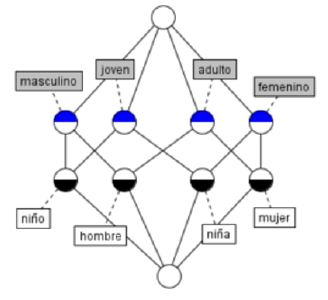
\includegraphics[height=.4\textheight,width=.55\textwidth]{ejemploReticulo.png}
%		\end{center}
%		\caption{Ejemplo de ret�culo de conceptos de un contexto formal.}
%		\label{figura:ejemploReticulo}
%	\end{figure}
%\end{minipage}

%\begin{table*}[tb]
%		\caption{Ejemplo de contexto formal utilizando datos reales del sector hotelero}
%		\label{table:hotelsExtract} 
%		\centering
%		{\scriptsize
%		\begin{tabular}{lccccccccc}
%			\hline
%			Nombre del Hotel & AC & Bar & Gym & Internet & Masajes & Parking\\
%			\hline
%			Fuerte Estepona Suites & X & X & X & X & X & X\\
%			Hotel Buenavista &  & X &  &  &  & X \\
%			Hotel Paraiso & X & X &  &  &  & X \\
%			Apts Marriot Playa &  &  &  & X &  &  \\
%			Hotel Piedra Paloma &  & X &  &  &  & X \\
%			Hostal Hospederia V Cent & X & X &  & X &  & X \\
%			\ldots\\
%			\hline
%		\end{tabular}
%		}
%	\end{table*}

%\begin{figure}[htbp]
%		\begin{center}
%			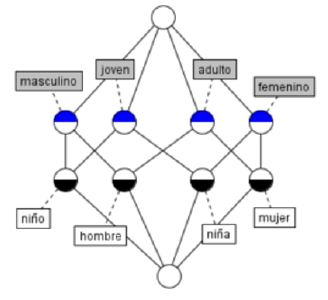
\includegraphics[height=.4\textheight,width=.55\textwidth]{ejemploReticulo.png}
%		\end{center}
%		\caption{Ejemplo de ret�culo de conceptos de un contexto formal.}
%		\label{figura:ejemploReticulo}
%	\end{figure}
	
\noindent
\begin{minipage}{\textwidth}
  \begin{minipage}[b]{0.4\textwidth}
    \centering
    {\scriptsize
    \begin{tabular}{ccccc}\hline
            & adulto & joven & femenino & masculino \\ \hline
       ni�o &  & X &  & X  \\
       ni�a &  & X & X &  \\
       hombre & X &  &  & X \\
       mujer & X &  & X &  \\
       \hline
      \end{tabular}
     }
      \captionof{table}{Ejemplo de contexto formal b�sico}
  \end{minipage}
  \hfill
  \begin{minipage}[b]{0.4\textwidth}
    \centering
    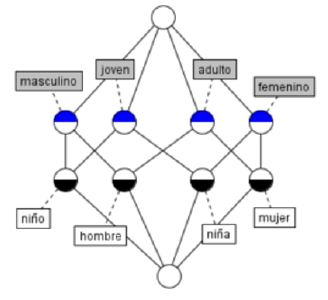
\includegraphics[height=.2\textheight,width=.9\textwidth]{ejemploReticulo.png} %\rule{6.4cm}{3.6cm}
    \captionof{figure}{Ret�culo de conceptos}
    \label{figura:ejemploReticulo}
  \end{minipage}
\end{minipage}

\vspace{0.3cm}

A partir del ret�culo de conceptos podemos obtener el contexto formal que representa. Los nodos del diagrama representan los objetos y atributos del contexto formal. Cada atributo del contexto corresponde a un elemento del ret�culo que tiene el conjunto de atributos minimal que contiene ese atributo, y un conjunto de objetos formado por todos los objetos con ese atributo. Por tanto, en la Figura \ref{figura:ejemploReticulo} estar�amos hablando de: masculino, joven, adulto y femenino. An�logamente, cada objeto del contexto corresponde a un elemento del ret�culo que est� formado por el conjunto de objetos minimal que contiene ese objeto, y un conjunto de atributos que consta de todos los atributos de dicho objeto. Esta vez, en la Figura \ref{figura:ejemploReticulo} nos referimos a: ni�o, hombre, ni�a y mujer.

Una alternativa gr�fica de definir los conceptos formales es la siguiente. Desde la representaci�n del contexto formal, un concepto formal se puede reconocer por medio de una submatriz de tal manera que todas las celdas de la submatriz son verdaderas (no es necesario que la submatriz est� formada por celdas contiguas). De esta forma, en la Tabla \ref{table:conceptosFormales}, vemos como podemos extraer un concepto formal como el par (\textit{\{Plymouth Satellite,Chevrolet Malibu\},\{Consumo, Cilindrada, Movilidad, Aceleraci�n\}}) a partir del contexto formal. 

\begin{table*}[tb]
\caption{Conceptos formales a partir de la representaci�n del contexto formal.}
\label{table:conceptosFormales} 
\centering
{\scriptsize
\begin{tabular}{lcccccc}
\hline
Modelo de coche & Consumo & Cilindrada & Movilidad & Potencia & Peso & Aceleraci�n\\
\hline
Chevrolet Vega &  &  &  & X &  & X\\
Toyota Corolla &  &  &  & X &  & \\
Ford Pinto &  &  & X &  & X & \\
Volkswagen Beetle & X &  & X & X & X & X \\
Plymouth Satellite  & \cellcolor{blue!25}X & \cellcolor{blue!25}X & \cellcolor{blue!25}X &  &  & \cellcolor{blue!25}X \\
Chevrolet Malibu & \cellcolor{blue!25}X & \cellcolor{blue!25}X & \cellcolor{blue!25}X &  &  & \cellcolor{blue!25}X \\
\hline
\end{tabular}
}
\end{table*}

Otra alternativa aparece en la representaci�n como grafo bipartito, donde un concepto formal aparece como un subgrafo bipartito completo, es decir, aquel que tiene todas las aristas posibles. Las conexiones que se establecen en el ret�culo nos indican que el objeto $X$ tiene un atributo $Y$ si y s�lo si existe un camino estrictamente creciente o estrictamente decreciente que permite ir de $X$ a $Y$ en el ret�culo.

Por otro lado, otro concepto equivalente a las conexiones de Galois y los operadores de cierre en el marco de FCA es el denominado sistema de implicaciones \cite{Ganter1997}. Como ya se adelant� en el Cap�tulo \ref{cap:introduccion}, las implicaciones constituyen el eje fundamental de trabajo en esta Tesis doctoral pues ser�n el mecanismo que nos permita abordar el problema del tratamiento eficiente de la informaci�n por medio de la l�gica. Reflejan una forma relativamente sencilla de trasladar las relaciones l�gicas que encontramos entre los atributos que poseen los objetos de nuestros datasets ya que combinan una forma muy simple y natural de escribir reglas del tipo \textit{si-entonces} con una gesti�n muy eficiente y automatizada de la informaci�n. 

Un ejemplo b�sico del uso de implicaciones para reflejar informaci�n contenida en los datos podemos verlo utilizando la informaci�n de la Tabla \ref{table:hotelsExtract}. En ese ejemplo vemos que en ese dataset hay una relaci�n que siempre se cumple y es la siguiente. Si el hotel provee servicio de aire acondicionado (AC) entonces tiene servicio de Parking. He ah� un claro ejemplo de regla \textit{si-entonces}, o en nuestro caso, de implicaci�n, que se verifica en el contexto.

Este concepto de implicaci�n es el que gu�a este trabajo otorg�ndonos un potencial para automatizar t�cnicas de razonamiento, con el beneficio que eso conlleva. Adem�s, las implicaciones son elemento fundamental para el desarrollo de formas m�s eficientes que el ret�culo de conceptos de representaci�n del conocimiento. 

%En la siguiente secci�n entraremos en detalle en el concepto de implicaci�n, daremos las definiciones formales necesarias y expondremos la l�gica que utilizaremos para sacar partido de ellas.

Por tanto, a partir de las implicaciones y de las propiedades b�sicas que verifican, podemos definir un c�lculo l�gico que nos permita realizar sistemas de deducci�n completos sobre el contexto actual. En cierto sentido, podr�amos decir que hemos pasado de tener un conocimiento basado en ejemplos a disponer de un conocimiento abstracto que introduce sistemas de razonamiento m�s elaborados, partiendo �nicamente de las observaciones concretas que hemos realizado, es decir, hemos aprendido reglas generales a partir de ejemplos.

Para finalizar, podemos considerar a las implicaciones, las conexiones de Galois y los operadores de cierre, como distintas alternativas de tratar la informaci�n que se puede extraer de un contexto formal. No obstante, las conexiones de Galois y los ret�culos de conceptos permiten una representaci�n gr�fica, mientras que los operadores de cierre y los sistemas implicacionales nos facilitan el razonamiento por medio de la l�gica.

En definitiva, todas estas nociones y propiedades son los fundamentos sobre los cuales se consolida FCA. Recordamos que la motivaci�n original de FCA es la reestructuraci�n de esta teor�a utilizando la teor�a matem�tica de conceptos y jerarqu�as con la intenci�n de acercarse al raciocinio humano y facilitar las conexiones con las L�gicas Filos�ficas del pensamiento \cite{Wille1982,Wille2005}.



\section{L�gica de Simplificaci�n}
\label{sec:logicaSimplificacion}
Introducimos la l�gica \slfde \cite{Enciso2002} describiendo sus cuatro pilares fundamentales: su lenguaje, su sem�ntica, su sistema axiom�tico y su m�todo de razonamiento autom�tico. 

\subsection*{Lenguaje}
\noindent
\begin{definicion}
	Dado un conjunto $M$ finito de s�mbolos (denominados atributos) no vac�o, el lenguaje sobre $M$ se define como: 
$$
\mathcal L_M:=\{A\to B\mid A,B\subseteq M\}
$$
\end{definicion}

Las f�rmulas $A \to B$ se denominan \emph{implicaciones} y los conjuntos $A$ y $B$ reciben el nombre de \emph{premisa} y \emph{conclusi�n} de la implicaci�n respectivamente. Los conjuntos $\sum \subseteq \mathcal L_M$ se denominan \emph{sistemas de implicaciones} sobre $M$.

Para simplificar la notaci�n:
\begin{itemize}
	\item Usaremos letras min�sculas para denotar los elementos en $M$, mientras que las may�sculas denotan sus subconjuntos.
	\item Omitimos las llaves en premisas y conclusiones, es decir, $abcde$ denota el conjunto $\{a,b,c,d,e\}$.
	\item Escribimos sus elementos por yuxtaposici�n, es decir, para $X \cup Y$ escribiremos $XY$.
	\item Para la diferencia, cambiamos $X-Y$ por $X \smallsetminus Y$.
\end{itemize}

\begin{definicion}[Implicaci�n]
	Una implicaci�n sobre un conjuntos de atributos $M$ es una expresi�n de la forma $X \to Y$, donde $X$ e $Y$ son conjuntos de atributos, i.e. $X \subseteq M$ y $Y \subseteq M$.
\end{definicion}

\begin{definicion}[Implicaci�n trivial]
	Una implicaci�n $X \to Y$ es trivial si $Y \subseteq X$.
\end{definicion}

\begin{definicion}[Implicaci�n unitaria]
	Sea $X$ un conjunto de atributos y $a$ un atributo del conjunto, $a \in X$, una implicaci�n se dice unitaria si su conclusi�n es un conjunto unitario, i.e. $X \to a$.
\end{definicion}

\begin{ejemplo}
	Sea $M = \{a,b,c,d\}$ un conjunto de atributos. Se cumple que $\{a\to b, a\to c\} \equiv \{a\to bc\}$ porque para cada contexto formal $\mathbf{K} := (G,M,I)$, se verifica que $\{b,c\}' = \{b\}' \cup \{c\}'$. Por tanto, $\{a\}' \subseteq \{b\}'$ y $\{a\}' \subseteq \{c\}'$ si y s�lo si $\{a\}' \subseteq \{b,c\}'$. Este ejemplo nos permite asegurar que cualquier sistema de implicaciones es equivalente a un sistema de implicaciones unitarias.
\end{ejemplo}

\begin{proposicion}
	Sea $M$ un conjunto de atributos y $\Sigma \subseteq \mathcal L_M$. Se verifica que:
	\[
		\Sigma \equiv \bigcup_{A\to B \in \Sigma} \{A \to b \mid b \in B\}
	\]
\end{proposicion}


\subsection*{Sem�ntica}
\noindent
Tras la definici�n del lenguaje pasamos ahora a introducir la sem�ntica utilizada, para lo cual utilizamos el concepto de \textit{operador de cierre} que reescribimos a continuaci�n.

Un operador de cierre en $M$ es una funci�n $c\colon 2^M \to 2^M$ que es \emph{extensivo} ($X\subseteq c(X) \ \forall X\subseteq M$), \emph{mon�tono} ($X_1\subseteq X_2$ implica que $c(X_1)\subseteq c(X_2)\ \forall X_1,X_2\subseteq M$), e \emph{idempotente} ($c(c(X))=c(X) \quad \forall X\subseteq M$). Los puntos fijos para $c$ (i.e. $X\subseteq M$ tales que $c(X)=X$) se denominan \emph{conjuntos cerrados}.

Un operador de cierre $c$ en $M$ recibe el nombre de \emph{modelo} para una implicaci�n $A\to B\in\mathcal L_M$ si $B\subseteq  c(A)$; se denota $c\models A\to B$. Adem�s, dado un sistema de implicaciones $\Sigma\subseteq \mathcal L_M$ y un operador de cierre $c$ en $M$, $c\models \Sigma$ denota que $c\models A\to B$ para todo $A\to B\in \Sigma$.

Decimos que $A\to B$ se \emph{deriva sem�nticamente} de $\Sigma$, denotado $\Sigma\models A\to B$, si cualquier modelo para $\Sigma$ tambi�n es un modelo para $A\to B$, i.e. $c\models \Sigma$ implica que $c\models A\to B$ para todo operador de cierre $c$ en $M$. 


\subsection*{Sistema Axiom�tico}
\noindent
Los conocidos Axiomas de Armstrong es el primer sistema descrito para tratar sistemas de implicaciones utilizando la l�gica. Tiene su origen en \cite{Armstrong74} donde se utiliz� para estudiar las propiedades de las dependencias funcionales en el modelo relacional de Codd \cite{Codd1970}. Este sistema ha tenido una clara influencia en el dise�o de varias l�gicas sobre implicaciones, todos ellas construidas alrededor del paradigma de la transitividad. Con el paso de los a�os, otros trabajos han propuesto sistemas axiom�ticos equivalentes \cite{Ibaraki1999,Atzeni1993,Paredaens89}.

Estos axiomas son v�lidos al generar s�lo implicaciones dentro del cierre del conjunto de implicaciones (denotado como $F^+$) cuando se act�a sobre el conjunto $F$. Tambi�n son completos ya que la aplicaci�n repetitiva de las reglas generar�n todas las implicaciones en el conjunto cerrado $F^+$. 

Este sistema axiom�tico est� formado por un axioma, denominado \textit{Reflexivo}, y dos reglas de inferencia, \textit{Aumentativa} y \textit{Transitiva} que se definen a continuaci�n

Sean $A$, $B$, $C$ subconjuntos de atributos de $M$. Entonces, tenemos:
%\begin{center}
%	{\scriptsize \tt{[Ref]}}\ {\footnotesize $\displaystyle\frac{}{AB \to A}$} \quad
%	{\scriptsize \tt{[Aug]}}\ {\footnotesize $\displaystyle\frac{A \to B\cup C}{AC \to BC}$} \quad
%	{\scriptsize \tt{[Tran]}}\ {\footnotesize $\displaystyle\frac{A \to B,\ B \to C}{A \to C}$ }
%\end{center}

\begin{center}
	{\scriptsize \tt{[Ref]}}\ $\displaystyle\frac{}{AB \to A}$ \quad
	{\scriptsize \tt{[Aug]}}\ $\displaystyle\frac{A \to B\cup C}{AC \to BC}$ \quad
	{\scriptsize \tt{[Tran]}}\ $\displaystyle\frac{A \to B,\ B \to C}{A \to C}$ 
\end{center}

Si bien es cierto que el sistema de Armstrong es un trabajo que acumula innumerables citas en diferentes trabajos a lo largo de los a�os, su utilidad pr�ctica se ve mermada debido a la dificultad que conlleva a la hora de plasmar las demostraciones. Es por ello que su uso est� enfocado al estudio te�rico de las implicaciones en vez de al desarrollo de nuevos algoritmos. No obstante, como se ha mencionado, es un buen punto de partida para el desarrollo de nuevas l�gicas para el tratamiento de las implicaciones. 

En este punto es donde aparece la \slfde \cite{Mora2004}, que constituye un marco mucho m�s adecuado en t�rminos de la automatizaci�n del razonamiento utilizando implicaciones. De hecho, \slfde ser� el n�cleo fundamental de los m�todos y las aplicaciones que se han llevado a cabo a lo largo de esta tesis doctoral.  

\slfde constituye una l�gica v�lida y completa \cite{Enciso2002} en la que el principal elemento del lenguaje son las implicaciones. Se define formalmente como:
\begin{definicion}%[Implicaci�n trivial]
	Sea $M$ un conjunto finito, la formulaci�n de \slfde son expresiones, denominadas implicaciones, de la forma $ X \to Y$, donde $X$ e $Y$ son subconjuntos de $M$.
\end{definicion}

Las implicaciones se interpretan de forma conjuntiva, es decir, corresponden a las f�rmulas $a_1\land \ldots\land a_n \to b_1\land \ldots\land b_m$ donde las proposiciones $a_1, \ldots  a_n,  b_1, \ldots, b_m$ son elementos del conjunto $M$. La interpretaci�n es la siguiente:

\begin{definicion}
Sea $O$ y $M$ dos conjuntos finitos, que representan objetos y atributos respectivamente, y $I$ una relaci�n en $O\times M$. Una implicaci�n de \slfde, $X\to Y$, donde $X$ y $Y$ son subconjuntos de $M$, es v�lida en $I$ si y s�lo si
$$\{o\in O\mid (o,x_i)\in I\, \ \forall x_i\in X\}\subseteq \{o\in O\mid (o,y_j)\in I\, \ \forall j_i\in Y\}$$
\end{definicion}

Adem�s de su forma natural de expresar el conocimiento como regla, las implicaciones proporcionan un sistema de razonamiento l�gico y de inferencia. Su tratamiento simb�lico se propuso como hemos mencionado anteriormente en \cite{Armstrong74}, sin embargo, debido al rol central que desempe�a la transitividad en ese sistema axiom�tico, el desarrollo de m�todos ejecutables para resolver problemas de implicaciones se basa en m�todos indirectos. \slfde evita el uso de la transitividad y se gu�a por la idea de simplificar el conjunto de implicaciones mediante la eliminaci�n atributos redundantes de manera eficiente  \cite{Mora2012}. Por consiguiente, la introducci�n de \slfde abri� la puerta al desarrollo de m�todos de razonamiento automatizados directamente basados en su novedoso sistema axiom�tico \cite{CorderoEMG14, CorderoEMOR15} que resumimos a continuaci�n.

\slfde se define como el par ($L_{FD}, S_{FD}$) donde $S_{FD}$ tiene el siguiente esquema axiom�tico:

\begin{center}
{\scriptsize \tt{[Ref]}}\quad $\displaystyle\frac{}{A\cup B \to A}$  
\end{center}

\noindent
junto con las siguientes reglas de inferencia, denominadas \emph{fragmentaci�n}, \emph{composici�n} y \emph{simplificaci�n} respectivamente.

%\begin{center}
%{\scriptsize \tt{[Frag]}}\ {\footnotesize $\displaystyle\frac{A\to B\cup C}{A\to B}$}  \quad
%{\scriptsize \tt{[Comp]}}\  {\footnotesize $\displaystyle\frac{A\to B,\ C \to D}{A\cup C \to B\cup D}$ } \quad
%{\scriptsize \tt{[Simp]}}\  {\footnotesize $\displaystyle\frac{A\to B,\ C \to D}{A\cup(C\smallsetminus B)\to D}$}
%\end{center}

\begin{center}
	{\scriptsize \tt{[Frag]}}\ $\displaystyle\frac{A\to B\cup C}{A\to B}$  \quad
	{\scriptsize \tt{[Comp]}}\ $\displaystyle\frac{A\to B,\ C \to D}{A\cup C \to B\cup D}$ \quad
	{\scriptsize \tt{[Simp]}}\ $\displaystyle\frac{A\to B,\ C \to D}{A\cup(C\smallsetminus B)\to D}$
\end{center}

Remarcamos que el lenguaje \slfde considera como f�rmulas v�lidas aquellas en donde cualquiera de sus dos partes puede ser el conjunto vac�o, denotado $A \to \varnothing$ y $\varnothing \to A$. Sus significados fueron discutidos en \cite{Enciso2002}. En ese trabajo, tambi�n presentamos el siguiente resultado donde la derivaci�n de una implicaci�n $A \to B$ se reduce a la derivaci�n de la f�rmula $\varnothing \to B$ teniendo $\varnothing \to A$. Este resultado se usar� m�s adelante en el dise�o de nuestro novedoso m�todo de cierre.

\begin{proposicion}
Para cualquier $\varGamma$ y $\forall X, Y\subseteq M$, $\varGamma \vdash X\to Y \text{ si y s�lo si }\varGamma \cup \{\top \to X\} \vdash\top \to Y$
\end{proposicion}


\begin{definicion}
Se dice que una implicaci�n $A\to B$ se deriva sint�cticamente de un sistema de implicaciones $\Sigma$, y se denota por $\Sigma\vdash A\to B$, si existe una secuencia de implicaciones $\sigma_1,\dots,\sigma_n \in \mathcal L_M$ tal que $\sigma_n=(A\to B)$ y, para todo $1\leq i\leq n$, la implicaci�n $\sigma_i$ satisface una de las siguientes condiciones:
	\begin{itemize}
		\item $\sigma_i$ es un axioma, es decir, verifica el esquema {\tt [Ref]}.
		\item $\sigma_i\in \Sigma$.
		\item $\sigma_i$ se obtiene a partir de implicaciones pertenecientes a $\{\sigma_j\mid 1\le j<i\}$ aplicando las reglas de inferencia {\tt [Frag]}, {\tt [Comp]} o {\tt [Simp]}.
	\end{itemize}
\end{definicion}

La secuencia $\sigma_1,\dots,\sigma_n$ constituye una \emph{demostraci�n} para $\Sigma\vdash A\to B$.

La derivaci�n sint�ctica proporciona una gesti�n automatizada de las implicaciones. En particular, se puede usar para resolver el denominado problema de las implicaciones: dado un conjunto de implicaciones $\Gamma$ y una implicaci�n $A\to B$, queremos responder si $A\to B$ se deduce de $\Gamma$. Este problema se puede abordar utilizando el operador de cierre.

El sistema axiom�tico es v�lido y completo, es decir, se cumple que la derivaci�n sint�ctica y sem�ntica coinciden. Esto significa que cada regla que se puede deducir con este sistema puede derivarse sem�nticamente (el sistema axiom�tico es v�lido) y viceversa (el sistema axiom�tico es completo).

\begin{theorem}
Sea $M$ un conjunto finito no vac�o de atributos, $\Sigma \subseteq \mathcal L_M$ y $A\to B \in \mathcal L_M$. Entonces, $\Sigma\models A\to B$ si y s�lo si $\Sigma\vdash A\to B$.  
\end{theorem}

La derivaci�n sint�ctica nos conduce a un nuevo operador de cierre denominado \textit{cierre sint�ctico}.

\begin{definicion}
	Dado un sistema de implicaciones $\Sigma \subseteq \mathcal L_M$, un conjunto $X \subseteq M$ se dice cerrado respecto de $\Sigma$ si $A \subseteq X$ implica $B \subseteq X$ para toda $A\to B\in \Sigma$. Debido a que $M$ es cerrado con respecto a $\Sigma$ y cualquier intersecci�n de conjuntos cerrados es cerrada, podemos definir el siguiente operador de cierre:
$$
(\ )^+_\Sigma\colon 2^M\to 2^M\qquad X^+_\Sigma=\bigcap\{Y\subseteq M\mid Y\text{ es cerrado con respecto a }\Sigma\text{ y }X\subseteq Y \}
$$
\end{definicion}

El siguiente teorema es esencial para calcular cierres y a su vez tambi�n para introducir un m�todo de razonamiento autom�tico.
 
\begin{theorem}[Teorema de deducci�n]\label{empty_set}
	Sea $A\to B\in\mathcal L_M$ y $\Sigma\subseteq \mathcal L_M$. Entonces, 
%\vspace*{-0.2cm}
	$$\Sigma \vdash A\to B \quad \mbox{sii} \quad B\subseteq A^+_\Sigma\quad \mbox{sii} \quad 
 	\{\varnothing\to A\} \cup \Sigma \vdash\{\varnothing\to B\}$$
\end{theorem}
 
\begin{corolario}
	Sea $\Sigma\subseteq \mathcal L_M$. $\forall X\subseteq M$, se tiene que 
	$$
	X^+_\Sigma=\max\{Y\subseteq M\mid \Sigma\vdash X\to Y \}.
	$$
\end{corolario}

La principal ventaja de \slfde radica en que las reglas de inferencia pueden considerarse reglas de equivalencia. Como consecuencia, \slfde se ha podido utilizar como n�cleo principal para el desarrollo de m�todos autom�ticos para diversas aplicaciones (e.g. obtener claves minimales, c�lculos del cierre) como veremos m�s adelante. Un estudio m�s detallado al respecto, incluyendo teoremas y demostraciones, puede verse en \cite{Mora2012}.


\subsection*{M�todo de Razonamiento Autom�tico}
\noindent
El problema de las implicaciones se ha abordado tradicionalmente utilizando un m�todo b�sico que recibe $A\subseteq M$ como entrada y utiliza de forma exhaustiva la
relaci�n de subconjuntos recorriendo iterativamente $\Gamma$ y agregando nuevos elementos al cierre. Este m�todo, propuesto en la d�cada de 1970 \cite{Maier83} y puede considerarse la base principal donde se han sustentado tantos otros. Podemos verlo detallado en el Algoritmo \ref{algoritmo:cierreUllman}.
\begin{algorithm2e}
%\footnotesize
%\SetAlgoLined
%\SetAlgoFuncName{SchemePruning}
%\dontprintsemicolon
%\KwIn{}
\KwData{$ \varGamma$, $A$}
\KwResult{$A^+_\Gamma$ }
%\KwOut{$X^+$}
    \Indp
    \Begin{
     $A^+_\Gamma:=A$
		
     \Repeat{$A^+_\Gamma=A^\prime$}{
        $A^\prime:=A^+_\Gamma$
				
       \ForEach{ $X \to Y \in  \varGamma$}{
           \If{$X \subseteq A^+_\Gamma$ {\bf and} $Y\not\subseteq A^+_\Gamma$}{
               $A^+_\Gamma:=A^+_\Gamma \cup \{Y\}$
           }%end if
       }% end foreach
		}%until 
   return $A^+_\Gamma$
   }%end begin
 \caption{Cierre cl�sico}
 \label{algoritmo:cierreUllman}
\end{algorithm2e}

M�s tarde, varios autores han desarrollado otros m�todos mediante el uso de diferentes t�cnicas, resolviendo eficientemente este problema en tiempo lineal. En \cite{Paredaens1989}, los autores muestran que la complejidad del problema de cierre es $\mathtt{O}(|{\mathcal{A}}|\, |{ \varGamma}|)$. En \cite{Mora2012}, presentamos un m�todo de cierre de atributos estrechamente relacionado con el sistema axiom�tico \slfde. Tambi�n demostramos que nuestro m�todo tiene un mejor rendimiento que aquellos basados en el cierre cl�sico.

Por nuestra parte, el m�todo de razonamiento autom�tico en \slfde se basa en el Teorema de Deducci�n y un conjunto de equivalencias. Siguiendo la forma habitual, dos sistemas de implicaciones $\Sigma_1,\Sigma_2\subseteq \mathcal L_M$ se dicen equivalentes si sus modelos coinciden, es decir, se cumple que para todo operador de cierre en $M$, $c\models \Sigma_1$ sii $c\models \Sigma_2$.

La siguiente proposici�n proporciona las tres equivalencias, denominadas tambi�n: \textit{Fragmentaci�n, Composici�n y Simplificaci�n}, que se se aplican y justifican el nombre de la l�gica \slfde porque, si las leemos de izquierda a derecha, eliminan la informaci�n redundante en el sistema de implicaciones (cf. \cite{Mora2012}).

\begin{proposicion}\label{simpl_equiv}
	Sean $A,B,C,D\subseteq M$. Se verifican las siguientes equivalencias:
	\begin{enumerate}
		\item {\small$\{A\to B\}\equiv\{A\to B\smallsetminus A\}$}
		\item {\small$\footnotesize\{A\to B, A\to C\}\equiv\{A\to B\cup C\}$}
		\item {\small$A\cap B=\varnothing$ y $A\subseteq C$ implica $\footnotesize\{A\to B, C \to D\}\equiv  \{A\to B, C\smallsetminus B\to D\smallsetminus B\}$}
\end{enumerate}
%
%\begin{equation*}
%\begin{split}
%\{X\to Y,\ U \to V\}& \equiv  \{X\to Y, (U-Y)\to(V-Y)\}\\
%\end{split}
%\end{equation*}
\end{proposicion}

Bas�ndonos en el Teorema de Deducci�n y las equivalencias anteriores, en \cite{Mora2012}, los autores presentan un novedoso algoritmo para calcular cierres utilizando \slfde, denominado {\tt Cls} que act�a seg�n el siguiente procedimiento.

Dado un conjunto $A\subseteq M$ y un conjunto de implicaciones $\Sigma$, {\tt Cls} calcula el par $(A^+_\Sigma,\Gamma)$, siendo $A^+_\Sigma$ el cierre sint�ctico de $A$ con respecto a $\Sigma$ y $\Gamma$ el conjunto residual de implicaciones respecto a $\varnothing \to A^+_\Sigma$. Esto permite determinar si una implicaci�n $A \to B$ puede deducirse de $\Sigma$.

Los pasos del algoritmo desglosados en lenguaje natural y de forma m�s detallada son:
\begin{itemize}
 \item En primer lugar, se incluye la f�rmula $\varnothing \to A$ en $\Sigma$ y se usa como semilla por el m�todo de razonamiento mediante las equivalencias mencionadas en la proposici�n anterior.
 \item A continuaci�n, el algoritmo entra en un proceso iterativo en el cual se ir�n aplicando las siguientes equivalencias mientras no se alcance la condici�n de parada.
	\begin{itemize}
		\item {\bf Eq. I}: Si $B\subseteq A$ entonces $\{\emptyset\to A,B\to C\} \equiv \{\emptyset\to A\cup C\}$.
		\item {\bf Eq. II}: Si $C\subseteq A$ entonces $\{\emptyset\to A,B\to C\} \equiv \{\emptyset\to A\}$.
		\item {\bf Eq. III}: En otro caso  $\{\emptyset\to A,B\to C\} \equiv \{\emptyset\to A,B\smallsetminus A\to C\smallsetminus A\}$.
	\end{itemize} 
 \item En el momento en el que no sea posible aplicar ninguna de las equivalencias anteriores, el algoritmo termina dando como resultado el conjunto cierre $A^+_\Sigma$, es decir, el cierre sint�ctico de $A$ con respecto a $\Sigma$, y adem�s, el conjunto residual de implicaciones $\Gamma$.
\end{itemize}

Formalmente, el algoritmo {\tt Cls} puede verse en la Funci�n \ref{algoritmo:Cls}.
\begin{function}[h]
\caption{Cls($A$,$\Sigma$) }\label{algoritmo:Cls}
\small
\DontPrintSemicolon
\SetKwInOut{Input}{input}
\SetKwInOut{Output}{output}
\Input{$A$, conjunto de atributos sobre los que se quiere calcular el cierre; \\
$\Sigma$, un sistema de implicaciones;}
\Output{$A^+_\Sigma$, cierre sint�ctico de $A$ con respecto a $\Sigma$; \\ 
$\Gamma$, el sistema de implicaciones residual;}
 
 
%    \Begin{

\Repeat{$\Gamma=\Sigma$}{
$\Gamma:=\Sigma$

$\Sigma:=\varnothing$
\ForEach{$B\to C\in \Gamma$}{
\lIf{$B\subseteq A$}{

\ \ \ \ {$A:=A\cup B$}
}
\lElseIf{$C\not\subseteq A$}{

\ \ \ \ {$\Sigma:=\Sigma\cup\{B\smallsetminus A\to C\smallsetminus A\}$}
}
}
}
 
     \Return $(A,\Gamma)$   
 
%   }%end begin
\end{function}


Aunque es cierto que existen en la literatura numerosas propuestas de algoritmos para calcular el cierre (la mayor�a de ellas como modificaciones del cierre cl�sico de Maier \cite{Maier83}), la principal novedad y ventaja que aporta {\tt Cls} es que, de manera simult�nea, tambi�n reducimos el n�mero de implicaciones, guardando el conocimiento complementario que describe la informaci�n que no pertenece al cierre. Este hecho nos coloca sin lugar a dudas en una posici�n privilegiada, ya que nos evita el elevado coste de un proceso de miner�a de datos para extraer el nuevo conjunto de implicaciones para el conjunto de datos reducido despu�s de cada aplicaci�n del m�todo, algo imprescindible cuando se utilizan las implementaciones cl�sicas. En consecuencia, el proceso supera los costos de miner�a de datos preservando una complejidad lineal a lo largo del proceso.

Finalizamos este apartado mostrando un ejemplo de aplicaci�n del algoritmo del cierre propuesto.

\begin{ejemplo}
\label{ejemplo:basico} 
	Sean $\Sigma=\{a\to c, bc\to d, c\to ae, d\to e\}$ y $A=\{c,e\}$. El algoritmo {\tt Cls} devuelve $A^+=\{a,c,e\}$. La siguiente tabla muestra la traza de ejecuci�n paso a paso del algoritmo. 

%{\small
$$\begin{array}{l||lllll}
\hline
Guide &  & \multicolumn{4}{c}{\Sigma } \\
%\hline
\emptyset\to ce &  & a\to c \quad& bc\to d \quad& c\to ae\quad& d\to e \quad\\
\hline
\hline
\emptyset\to ce &   & a\to \!\!\not\! c & b\!\!\not\! c\to d & \!\!\not\! c\to a\!\!\not\! e& d\to \!\!\not\! e \\
\emptyset\to ace &   &  & b\to d & & \\
%\emptyset\to acef &   &  & b\to d &  & \\
\hline
\end{array}
$$
%}%end small

Por tanto, una vez finalizado la ejecuci�n del algoritmo, obtenemos: ${\tt Cls}(\{c,e\},\{a\to c, bc\to d, c\to ae, d\to e\})=(\{a,c,e\},\{b\to d\})$, donde el cierre es $\{c,e\}^+_\Sigma = \{a,c,e\}$  y el conjunto residual de implicaciones queda como:  $\Gamma = \{b \to d\}$.
\end{ejemplo}%

% =====================================================================
% =====================================================================
% =====================================================================
\clearemptydoublepage
\pagestyle{empty}

\clearemptydoublepage
%%

\part{Claves y Generadores Minimales}

% this file is called up by thesis.tex
% content in this file will be fed into the main document

\pagestyle{empty}
%: ----------------------- name of chapter  -------------------------
\chapter{Claves Minimales}
\label{cap:clavesMinimales} % top level followed by section, subsection


%: ----------------------- paths to graphics ------------------------

% change according to folder and file names
%\ifpdf
%    \graphicspath{{X/figures/PNG/}{X/figures/PDF/}{X/figures/}}
%\else
%   \graphicspath{{X/figures/EPS/}{X/figures/}}
%\fi

%: ----------------------- contents from here ------------------------


\pagestyle{headings}

\bigdrop{0pt}{5}{cmr10}Identificar las claves de un esquema relacional es una tarea imprescindible dentro de numerosas �reas diferentes de la gesti�n de la informaci�n. Ejemplos de ello nos remontan incluso d�cadas atr�s, donde podemos ver que las claves constituyen un elemento fundamental en acciones como pueden ser: la optimizaci�n de consultas \cite{Kemper1991}, el indexado \cite{Kemper1991} o el modelado de datos \cite{Simsion2005}, pero el concepto y sus aplicaciones son igualmente extensibles a sistemas actuales. 

Generalmente, es tarea de ingenier�a establecer y elegir las claves como parte de la normalizaci�n del esquema. El reto es encontrar esos atributos del esquema que nos permitan identificar de forma �nica cada tupla de la relaci�n.

% Clave
T�cnicamente, una clave de un esquema relacional est� compuesta por un subconjunto de atributos que act�an como el dominio de una funci�n cuya imagen es el propio conjunto de atributos. Estas funciones se describen como dependencias funcionales (en adelante FD, por sus siglas en ingl�s, \textit{Functional Dependencies}), las cuales especifican una restricci�n entre los dos conjuntos de atributos, que denotamos como $A \rightarrow B$, y que nos asegura que para cualquier tupla de la relaci�n, si la tupla verifica el antecedente $A$, entonces tambi�n verifica el consecuente $B$. Tal y como hemos visto en los cap�tulos introductorios, este definici�n coincide exactamente con el concepto de \textit{if-then rules} que hasta ahora hemos introducido seg�n la denominaci�n de implicaci�n por hallarnos en el marco de FCA, sin embargo, esta vez, la diferencia de nombre se debe simplemente al entorno en el que ahora vamos a trabajar, esto es, las bases de datos relacionales, donde se habla de dependencias funcionales para este tipo de reglas. Se expone formalmente en las siguientes definiciones.

\begin{definicion}[Atributo]
Un atributo $A$ es un identificador para un elemento en un dominio $D$.
\end{definicion}

\begin{definicion}[Dependencia funcional]
Sea $\Omega$ un conjunto de atributos. Una dependencia funcional (FD) sobre $\Omega$ es una expresi�n de la forma $X \rightarrow Y$, donde $X, Y\subseteq \Omega$. Se satisface en una tabla $R$ siempre y cuando para cada dos tuplas de $R$, si verifican $X$, entonces tambi�n verifican $Y$.
\end{definicion}

\begin{definicion}[Dependencia funcional trivial]
Sea $\Omega$ un conjunto de atributos. Una dependencia funcional (FD) $X \rightarrow Y$ sobre $\Omega$, se denomina trivial si $Y\subseteq X$.
\end{definicion}

\begin{definicion}[Dependencia funcional unitaria]
Sea $\Omega$ un conjunto de atributos. Una dependencia funcional (FD) $X \rightarrow Y$ sobre $\Omega$, se denomina unitaria si $Y$ es un conjunto unitario.
\end{definicion}

Las claves nos permiten identificar de forma un�voca cada una de las tuplas que existan en una relaci�n y podemos definirlas por medio de FD como sigue:

\begin{definicion}[Clave]
Dada un tabla $R$ sobre un conjunto de atributos $\Omega$, decimos que $K$ es un clave de $R$ si se verifica la dependencia funcional $K\rightarrow \Omega$ en $R$.
\end{definicion}

Una caracter�stica muy importante de la claves es su minimalidad. Una clave se considerar� minimal cuando todos y cada uno de los atributos que la forman son imprescindibles para mantener su naturaleza de clave, es decir, no contiene ning�n atributo superfluo. Formalmente:

\begin{definicion}[Clave minimal]
Dada un tabla $R$ sobre un conjunto de atributos $\Omega$, decimos que $K$ es una clave minimal de $R$ si se verifica la dependencia funcional $K\rightarrow \Omega$ en $R$ y $\not\exists a \in K$ tal que $K \smallsetminus \{a\} \rightarrow \Omega$.
\end{definicion}

\begin{remark}
Es de vital importancia mencionar que aunque para averiguar el conjunto de claves vamos a trabajar sobre FDs, no es objetivo de esta Tesis extraerlas a partir de un esquema relacional. Para ello, existen desde hace tiempo numerosas t�cnicas en la literatura que se ocupan de realizar esta tarea \cite{HuhtalaKPT99,YaoHB2002,Yevtushenko2006}. Por tanto, haremos uso de estas t�cnicas a la hora de enfrentarnos con un esquema relacional para obtener el conjunto de FD que se verifican sobre esos datos de forma que tengamos la semilla sobre la que aplicar las t�cnicas de b�squeda de claves que son motivo de estudio en esta tesis.
\end{remark}

Para ilustrar de forma b�sica el concepto de clave, vamos a utilizar el siguiente Ejemplo \ref{ejemplo:basicoClaves}.

\begin{ejemplo}
\label{ejemplo:basicoClaves}
Supongamos que disponemos de la Tabla \ref{tabla:ejemploPeliculas}. Es una peque�a tabla donde se refleja informaci�n que relaciona t�tulos de pel�culas, actores, pa�ses, directores, nacionalidad y a�os de estreno. 

De esta informaci�n, utilizando los m�todos comentados anteriormente, podemos extraer el siguiente conjunto de FDs: 

$\Gamma = \{Titulo, A\tilde{n}o \rightarrow Pais$;  $Titulo, A\tilde{n}o \rightarrow Director$; $Director\rightarrow Nacionalidad$\}. 

\begin{table*}[htbp]
\caption{Tabla de pel�culas}
\label{tabla:ejemploPeliculas}
\centering
{\scriptsize
\begin{tabular}{cccccc}
 \hline
 T�tulo & A�o & Pa�s & Director & Nacionalidad & Actor\\
 \hline
 Pulp Fiction & 1994 & USA & Quentin Tarantino & USA & John Travolta\\
 Pulp Fiction & 1994 & USA & Quentin Tarantino & USA & Uma Thurman\\
  Pulp Fiction & 1994 & USA & Quentin Tarantino & USA &Samuel Jackson \\
 King Kong & 2005 & NZ & Peter Jackson& NZ & Naomi Watts\\
 King Kong & 2005 & NZ & Peter Jackson & NZ & Jack Black\\
 King Kong & 1976 & USA & De Laurentiis & IT & Jessica Lange\\
 King Kong & 1976 & USA & De Laurentiis & IT & Jeff Bridges\\
 Django Unchained & 2012 & USA & Quentin Tarantino  & USA & Jamie Foxx\\
 Django Unchained & 2012 & USA & Quentin Tarantino  & USA & Samuel Jackson\\\hline
\end{tabular}
}
\end{table*}

Esta tabla tiene una sola clave minimal: $\{Titulo, A\tilde{n}o, Actor\}$ que corresponde con el conjunto de atributos necesario para identificar cualquier tupla de la relaci�n.
\end{ejemplo}

Aquellos lectores que no est�n familiarizados con las nociones formales de FD, claves y tablas relacionales pueden consultar uno de los trabajos m�s citados al respecto en \cite{Elmasri2010}.

Es conveniente aclarar que el trabajo llevado a cabo no es una cuesti�n de miner�a de datos \cite{Fay96}. De forma muy general podr�amos decir que la miner�a de datos puede considerarse un proceso computacional para descubrir patrones en grandes vol�menes de datos con el objetivo de extraer informaci�n de un conjunto de datos y transformarla en estructuras para diversos usos \cite{witten2011}. Sin embargo, nuestra labor consiste en desarrollar, a partir de la informaci�n ya extra�da de los datos, los mecanismos y algoritmos necesarios para encontrar las claves de los conjuntos de datos, y en general, descubrir el conocimiento impl�cito, que nos permitan realizar un tratamiento m�s inteligente y eficiente de la informaci�n. 

En este cap�tulo, analizaremos el problema de la b�squeda de claves \ref{sec:problemaBusquedaClaves} y el estado del arte \ref{sec:metodosSSTCK}, pero antes vamos a mostrar algunas situaciones donde la existencia de este problema es relevante \ref{sec:aplicaciones}. Cerrar�n este cap�tulo dos secciones m�s; la primera es realmente importante ya que presenta la implementaci�n de los m�todos y la filosof�a de computaci�n paralela que se ha utilizado \ref{seccion:implementacion} y en la �ltima se recogen en diversas tablas los resultados obtenidos por cada uno de los m�todos \ref{seccion:experimentosResultados}.



\section{Aplicaciones}
\label{sec:aplicaciones}
Antes de seguir avanzando, es momento de apoyar el valor intr�nseco de los datos mostrando una situaciones de ejemplo donde conocer las claves del sistema es fundamental.

\begin{ejemplo}
\label{ejemplo:basicoAplicacionClaves}
Sea el caso en que tenemos almacenados los datos personales de los empleados de una determinada empresa (e.g. nombre, edad, DNI, tel�fono, etc.). Se podr�a pensar que una forma de identificar a uno de los empleados podr�a ser a trav�s de su nombre y apellidos. Sin embargo, esto no ser�a correcto puesto que hay personas diferentes cuyos nombres y apellidos pueden coincidir. Tal podr�a ser el caso de nombres m�s habituales tanto dentro del territorio nacional como Antonio Fern�ndez o fuera, como Peter Williams. Otra alternativa podr�a ser elegir el n�mero de tel�fono, pero tambi�n podr�a ser un fallo en tanto en cuanto una misma familia o compa�eros de trabajo pueden compartir el mismo n�mero de l�nea fija de tel�fono. 
\end{ejemplo}

En este ejemplo, el elemento que nos permite identificar de forma �nica a un empleado es el DNI, y por tanto, �sa debe ser la clave de nuestro esquema. Y adem�s, puesto que solamente contiene la informaci�n necesaria para ser clave, estamos ante una clave minimal. Sin embargo, no es la �nica clave que existe. Pensemos que si tomamos combinaciones de valores como \textit{DNI} y \textit{Apellidos}, tambi�n estar�amos obteniendo una clave v�lida del esquema, pero en este caso, puesto que tenemos informaci�n que no es imprescindible (e.g. \textit{Apellidos}), no estar�amos ante una clave minimal.


\begin{ejemplo}[Optimizaci�n de consultas]
Dependiendo del sistema de informaci�n con el que estemos tratando, la complejidad que pueden alcanzar algunas consultas puede ser tal que su tiempo de respuesta no sea admisible. Un ejemplo de una consulta de cierta complejidad dentro de un hipot�tico modelo sanitario a nivel nacional, podr�a consistir en solicitar al sistema la lista de los varones mayores de 40, que hayan tenido al menos una intervenci�n quir�rgica, est�n casados, posean vivienda propia, tengan al menos dos hijos, ... 
\end{ejemplo}

Este tipo de consultas pueden necesitar acceder a tal cantidad de recursos que a la hora de obtener una respuesta del sistema, el tiempo de espera puede ser intratable. Por tanto, tener el sistema bien dise�ado de manera que las consultas se puedan hacer de forma eficiente ser� un aspecto fundamental del sistema; una de las formas principales de conseguir esto es mediante un buen dise�o que nos permita decidir a trav�s de qu� elementos dirigir la b�squeda, es decir, conocer las claves del modelo de datos \cite{Elmagarmid2007}.

\vspace{0.3cm}
Un aspecto muy importante en las tecnolog�as de la informaci�n es tener mecanismos que nos permitan detectar errores que pueden producirse en la gesti�n y almacenamiento de la informaci�n. Estos errores pueden deberse a multitud de causas y no s�lo se producen a la hora de dise�ar un nuevo sistema, sino que pueden aparecer a lo largo del tiempo de vida de un sistema ya sea por el uso prolongado, cambios en las tecnolog�as, la intervenci�n de diferentes personas, etc. En estos casos, es imprescindible tener mecanismos para encauzar la b�squeda del error y para ello, es fundamental conocer las claves del sistema \cite{Atencia2012}. Para mostrar una situaci�n en la que conocer las claves nos puede ayudar en la detecci�n de errores supongamos la siguiente situaci�n.

\begin{ejemplo}[Detecci�n de errores]
Suele ser com�n que se produzcan errores en bases de datos debido a las peculiaridades de algunos nombres personales. Los m�s comunes suelen ser la repetici�n de registros. Por ejemplo, pensemos una editorial que tenga una base de datos enorme de art�culos cient�ficos donde se almacena simplemente el nombre de los autores y el de las publicaciones. Ahora, pongamos por caso que en una publicaci�n el nombre de uno de los autores es Aurora Manj�n Ramos, mientras que en otra perteneciente a la misma autora, el nombre registrado es Aurora Manj�n-Ramos. Si queremos obtener las aportaciones de este autor en este sistema, habr� que tener en cuenta la sutil diferencia en la forma de los apellidos pues de lo contrario la lista de art�culos no ser� consistente. 
\end{ejemplo}

Esto ocurre porque el sistema est� abierto al fallo humano al no tener mecanismos para bloquear la posible duplicidad de registros. Actualmente y en relaci�n a este caso particular, el sistema de control DOI elaborado por la Corporaci�n Nacional para Iniciativas de Investigaci�n (CNRI) es un claro ejemplo de una forma de clave con la que identificar los trabajos. En definitiva, poseer una clave que nos determine c�mo se introduce nueva informaci�n en el sistema ser� esencial para evitar este tipo de situaciones de error.



\section{El problema de la b�squeda de claves}
\label{sec:problemaBusquedaClaves}
% Problema de la b�squeda de claves
El problema de la b�squeda de claves consiste en encontrar todos los subconjuntos de atributos que componen una clave m�nimal a partir de un conjunto de FD que se verifican en un esquema de una tabla de de datos relacional. Es un campo de estudio con d�cadas de antig�edad en el que podemos remontarnos a un primer estudio preliminar en \cite{Fadous75}, donde las claves se estudiaron dentro del �mbito de la matriz de implicaciones u otros tantos trabajos como \cite{Sali2004,Giannella99} que se centran en averiguar estas claves minimales.

% Claves como elemento crucial
Las claves constituyen un elemento crucial en cualquier modelo de datos, incluyendo el modelo de datos relacional de Codd \cite{Codd1970}. Sin embargo, la dificultad al enfrentarnos con el problema de la b�squeda de claves surge debido a que, dado un conjunto de atributos $A$, la cardinalidad del conjunto $2^A$ hace que haya que abordar el problema aplicando t�cnicas que gu�en la b�squeda de los conjuntos candidatos a ser claves minimales. 

% problema NP
El c�lculo de todas las llaves minimales representa un problema complejo. En \cite{Lucchesi78,Yu76} se incluyen resultados interesantes acerca de la complejidad del problema; los autores demuestran que el n�mero de claves minimales para un sistema relacional puede ser exponencial respecto al n�mero de atributos, o factorial respecto al n�mero de dependencias. Adem�s, establecieron que el n�mero de claves est� limitado por el factorial del n�mero de dependencias, por tanto, no existe un algoritmo que resuelva el problema en tiempo polin�mico. Hay otros resultados que apoyan la complejidad del problema; es un problema NP-completo decidir si existe una clave de tama�o a lo sumo $k$ dado un conjunto de FD \cite{Lucchesi78}.

% referencias generales
Las principales referencias sobre este problema apuntan a los trabajos de Lucchesi y Osborn en \cite{Lucchesi78} que muestran un algoritmo para calcular todas las claves candidatas. Por otro lado, Saiedian y Spencer \cite{Saiedian1996} presentaron un algoritmo usando grafos con atributos para encontrar todas las claves posibles de un esquema de base de datos relacional. No obstante, demostraron que s�lo pod�a aplicarse cuando el grafo de FDs no estuviera fuertemente conectado. Otro ejemplo lo encontramos en el trabajo de Zhang \cite{Zhang09} en el cual se utilizan mapas de Karnaugh \cite{Karnaugh1953} para calcular todas las claves. Tambi�n existen trabajos m�s recientes sobre el c�lculo de las claves minimales como son \cite{Sismanis2006,Worland2004} y otra contribuci�n actual que aborda el problema en un estilo l�gico \cite{CorderoEMG14}. Asimismo, en \cite{Levy2005,Valtchev03,Valtchev08} los autores propusieron el uso de FCA \cite{Ganter1997} para abordar problemas relacionados con la b�squeda y la gesti�n de las implicaciones, que pueden considerarse complementarios a nuestro trabajo.

Es significativo como el problema de la b�squeda de claves aparece en diversos campos de conocimiento. Por ejemplo, en \cite{Benito-PicazoCMMSE2015} se hace menci�n a la importancia de conocer las claves en �reas emergentes como el \textit{linked-data}. Por otro lado, en \cite{CorderoEMG14}, mostramos c�mo el problema de las claves m�nimales en las bases de datos tiene su an�logo en FCA, donde el papel de las FDs se manifiesta, como ya hemos comentado, como implicaciones de atributos. En ese art�culo, el problema de las claves m�nimales se present� desde un punto de vista l�gico y para ello se emple� un sistema axiom�tico para gestionar las FDs y
las implicaciones; este sistema es el que en apartados anteriores hemos presentado como \slfde \cite{Enciso2002}.

% referencias de tableaux
En nuestro objetivo de esta parte de la Tesis nos vamos a concentrar en los algoritmos de b�squeda de claves basados en la l�gica, y m�s espec�ficamente, en aquellos que utilizan el paradigma de Tableaux \cite{Morgan1992} para determinar las claves de un esquema relacional utilizando un sistema de inferencia. 

%De forma muy general, podemos considerar al Tableaux como un �rbol de b�squeda cuyas ramas se van formando por la acci�n de diferentes reglas de inferencia y cuyas hojas contienen las claves del esquema relacional original.

De forma muy general, podemos decir que los m�todos tipo Tableaux representan el espacio de b�squeda como un �rbol, donde sus hojas contienen las soluciones (claves). El proceso de construcci�n del �rbol comienza con una ra�z inicial y desde all�, las reglas de inferencia generan nuevas ramas etiquetadas con nodos que representan instancias m�s simples del nodo padre. La mayor ventaja de este proceso es su versatilidad, ya que el desarrollo de nuevos sistemas de inferencia nos permiten dise�ar un nuevo m�todo. Las comparaciones entre estos m�todos se pueden realizar f�cilmente ya que su eficiencia va de la mano con el tama�o del �rbol generado.

Esto nos lleva a un punto de partida fundamental, los estudios de R. Wastl (Universidad de Wurzburg, Alemania) \cite{Wastl98a,Wastl98} donde se introduce por primera vez un sistema de inferencia de tipo Hilbert para averiguar todas las claves de un esquema relacional. A modo de ejemplo b�sico, en la Figura \ref{figura:ejemploTaleaux} podemos ver un ejemplo de �rbol de b�squeda seg�n el paradigma de Tableaux desarrollado seg�n las reglas de inferencia del sistema de inferencia $\mathbb{K}$ de Wastl.

\begin{figure}[htbp]
	\begin{center}
		\includegraphics*[width=.75\textwidth,height=.3\textheight]{arbol897.png}
	\end{center}
	\caption{Ejemplo de Tableaux utilizando el sistema de inferencia $\mathbb{K}$ de Wastl.}
	\label{figura:ejemploTaleaux}
\end{figure}

Siguiendo esta l�nea, en \cite{Cordero2013} los autores abordan el problema de la b�squeda de claves utilizando un sistema de inferencia basado en la l�gica de simplificaci�n para dependencias funcionales \cite{Enciso2002}. En \cite{Mora2012} los autores muestran la equivalencia entre \slfde y los axiomas de Armstrong \cite{Armstrong74} junto con un algoritmo para calcular el cierre de un conjunto de atributos. Los autores tambi�n exponen una comparaci�n con otros algoritmos del cierre que aparecen en la literatura para demostrar la orientaci�n pr�ctica del sistema l�gico.

M�s tarde, en \cite{CorderoEMG14}, los autores introdujeron el m�todo SST, basado en la introducci�n del test de minimalidad que evita la apertura de ramas adicionales del �rbol, por lo que el espacio de b�squeda se vuelve m�s reducido, logrando un gran rendimiento en comparaci�n con sus predecesores.

% con el paralelo
Recordemos que para abordar el problema de la b�squeda de claves en grandes sistemas, nuestro objetivo era utilizar las t�cnicas l�gicas sobre una implementaci�n paralela de los m�todos que, mediante el uso de recursos de supercomputaci�n, nos permitan alcanzar resultados en un tiempo razonable. En esta l�nea, son varios los trabajos que han utilizado la paralelizaci�n para afrontar problemas relacionados con implicaciones o FCA. Un algoritmo paralelo para el tratamiento de implicaciones enmarcado en el campo de los hipergrafos lo podemos encontrar en \cite{Sridhar1990}. A su vez, Krajca et al. \cite{Krajca2008} presentan un algoritmo paralelo para el c�lculo de conceptos formales. Por nuestra parte, una primera aproximaci�n a la paralelizaci�n del m�todo de Wastl \cite{Wastl98a,Wastl98} y el algoritmo de claves \cite{Cordero2013} fue presentado en \cite{Benito-Picazo2014}, donde se muestra c�mo el paralelismo puede integrarse de forma natural en los m�todos basados en tableaux. Fue este el punto de partida para el desarrollo de los nuevos m�todos m�s eficientes que vemos a continuaci�n.




\section{Algoritmos para el c�lculo de claves}
\label{sec:metodosSSTCK}
% nuestra contribuci�n
Nuestra contribuci�n principal en relaci�n a esta parte de la tesis se produce de la siguiente forma. Bas�ndonos en el sistema axi�matico de la l�gica \slfde \ref{sec:logicaSimplificacion}, proponemos un nuevo m�todo llamado \textit{Closure Keys (CK)} que incorpora un mecanismo eficiente de poda que utiliza el m�todo de cierre basado en \slfde para mejorar el m�todo SST. El nuevo m�todo se basa en la relaci�n fuerte entre la noci�n de clave y el operador de cierre, no s�lo a nivel de definici�n, sino tambi�n en cuanto a su construcci�n. 

El operador de cierre definido en \cite{Mora2012} y que hemos introducido previamente en el cap�tulo de Preliminares \ref{cap:preliminares} como \cierre, nos permite reducir el espacio de b�squeda realizando reducciones en el camino hacia las hojas, donde finalmente se obtienen las claves. Adem�s, se ha desarrollado una implementaci�n paralela tanto del m�todo SST como del m�todo CK junto con varios experimentos, los cuales necesitan llevarse a cabo en entornos de supercomputaci�n, para confirmar las mejoras que se han alcanzado.


\subsection*{M�todo SST}
\label{subsec:metodoSST}
En \cite{CorderoEMG14} se present� un nuevo algoritmo, denominado SST, para calcular todas las claves minimales usando una estrategia de estilo tableaux, abriendo la puerta a incorporar el paralelismo en su implementaci�n. SST se basa en la noci�n de cierre de conjunto, una noci�n b�sica en la teor�a de base de datos que permite caracterizar el conjunto m�ximo de atributos que se puede alcanzar, desde un determinado conjunto de atributos $A$ con respecto a un conjunto de FD, utilizando el sistema axiom�tico. Por lo tanto, si el cierre de $A$ se denota como $A^+_\Gamma$, el sistema de inferencia para FD nos permite inferir la FD $A\to A^+_\Gamma$. El enfoque con estilo l�gico para el problema de las claves minimales consiste en la enumeraci�n de todos los conjuntos de atributos $A$ tales que se verifique la FD: $A\to\Omega$.

El m�todo SST presenta dos mejoras fundamentales con respecto a sus predecesores. En primer lugar, consigue una reducci�n en el n�mero de ramas y la segunda mejora consiste en el desarrollo de potentes reglas de inferencia que reducen la profundidad de las ramas, lo cual acelera significativamente la b�squeda de las claves.
Estas dos nuevas reglas de inferencia, denominadas {\tt{[sSimp]}} y {\tt{[lSimp]}} y que se muestran a continuaci�n son dos extensiones concretas de la regla de simplificaci�n de la \slfd. 

\[[sSimp] \quad \frac{A \rightarrow B \quad C \rightarrow D}{A(C \smallsetminus B) \rightarrow D \smallsetminus AB} \quad [lSimp] \quad \frac{A \rightarrow B \quad C \rightarrow D}{A(C \smallsetminus B) \rightarrow D}\]

Estas reglas gu�an la construcci�n del espacio de b�squeda para descubrir todas las claves minimales \cite{CorderoEMG14}. El m�todo avanza paso a paso construyendo un �rbol desde el problema original hasta llegar a las hojas donde encontramos las soluciones, es decir, las claves. Las reglas se aplican a cada par (conjunto de atributos, conjunto de implicaciones) correspondiente a cada nodo del �rbol para producir nuevos nodos en un nivel inferior, que ser�n el origen de nuevas ramas del �rbol de b�squeda. 

Al aplicar {\tt{[lSimp]}} sobre el subconjunto de atributos en cada nodo y la implicaci�n en el borde correspondiente, obtenemos la nueva ra�z en la rama. Por ejemplo, en la Figura \ref{figura:aplicacionAlgoritmoCK}, a partir de $\Omega$ y $A_1\to B_1$, obtenemos el nuevo subconjunto $\Omega_1$.

\begin{figure}[htbp]
	\begin{center}
		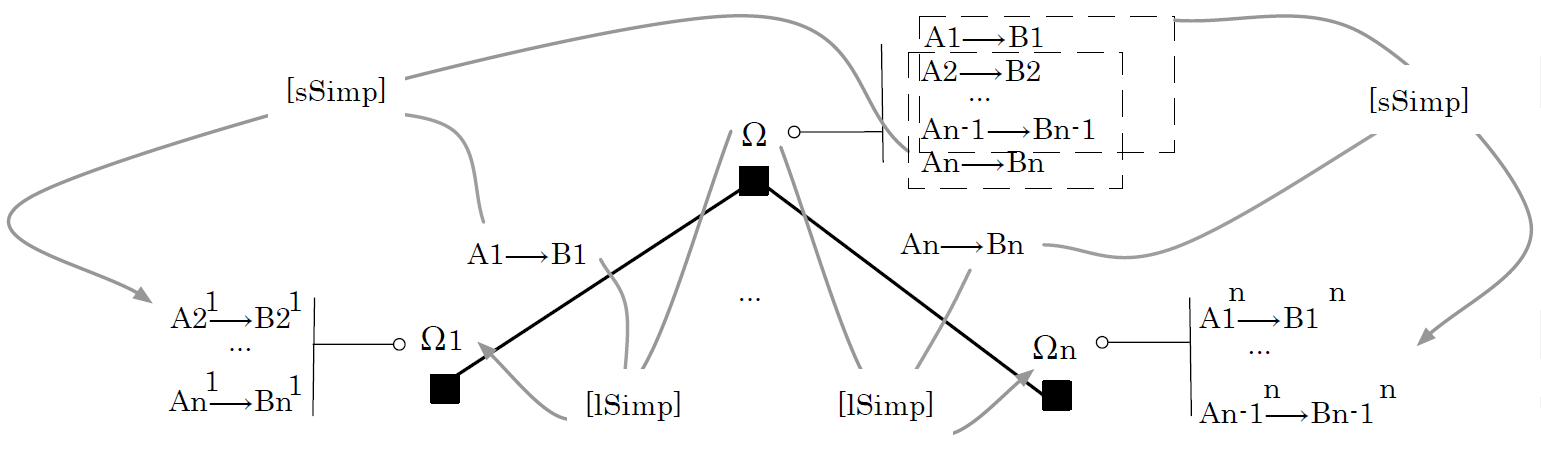
\includegraphics[height=.2\textheight,width=.95\textwidth]{aplicacionAlgoritmoCK.png}
	\end{center}
	\caption{Aplicaci�n de las reglas {\tt{[sSimp]}} y {\tt{[lSimp]}} en el algoritmo \textit{Closure Keys}.}
	\label{figura:aplicacionAlgoritmoCK}
\end{figure}

Por otra parte, la aplicaci�n de {\tt{[sSimp]}} sobre la implicaci�n establecida en cada nodo se hace tomando cada implicaci�n como pivote y aplicando la regla al resto de las implicaciones para generar nuevas ramas. Podemos verlo en la Figura \ref{figura:aplicacionAlgoritmoCK}, donde la primera rama se genera tomando $A_1\to B_1$ como pivote y aplic�ndolo al resto de implicaciones $A_2\to B_2,\ldots,A_n\to B_n$. Cuando el conjunto de implicaciones en un nodo es el conjunto vac�o, hemos llegado a una hoja del �rbol y por tanto, a una clave, que agregamos a la soluci�n global. A continuaci�n mostramos un ejemplo completo de aplicaci�n.

\begin{ejemplo}
\label{ejemploTableauxGrande}
Sea un conjunto de atributos $U = \{a,b,c,d,e,g\}$ y un conjunto de implicaciones $\Gamma = \{ab \rightarrow c, bc \rightarrow d, be \rightarrow c, cg \rightarrow b, c \rightarrow a, d \rightarrow eg, ce \rightarrow g\}$. El conjunto $K$ de todas las claves minimales que se extraen es $K = \{cd, bc, ce, cg, bd, ab, be\}$ y el Tableaux que se genera pondemos verlo en la Figura \ref{figura:arbolGrande}. 

Obs�rvese que el primer nivel del �rbol tiene s�lo cuatro hijos, que corresponden a las cuatro f�rmulas minimales en $\Gamma$. En el caso del m�todo \slfde estar�amos hablando de 7 hijos en este primer nivel. La eficaz estrategia proporcionada por el m�todo SST y sus nuevas reglas de inferencias redunda en el �xito en la construcci�n de todo el �rbol. De esta forma, el �rbol final tiene 21 nodos mientras que en el caso del m�todo \slfde hablamos de 244.

\begin{figure}[htbp]
	\begin{center}
		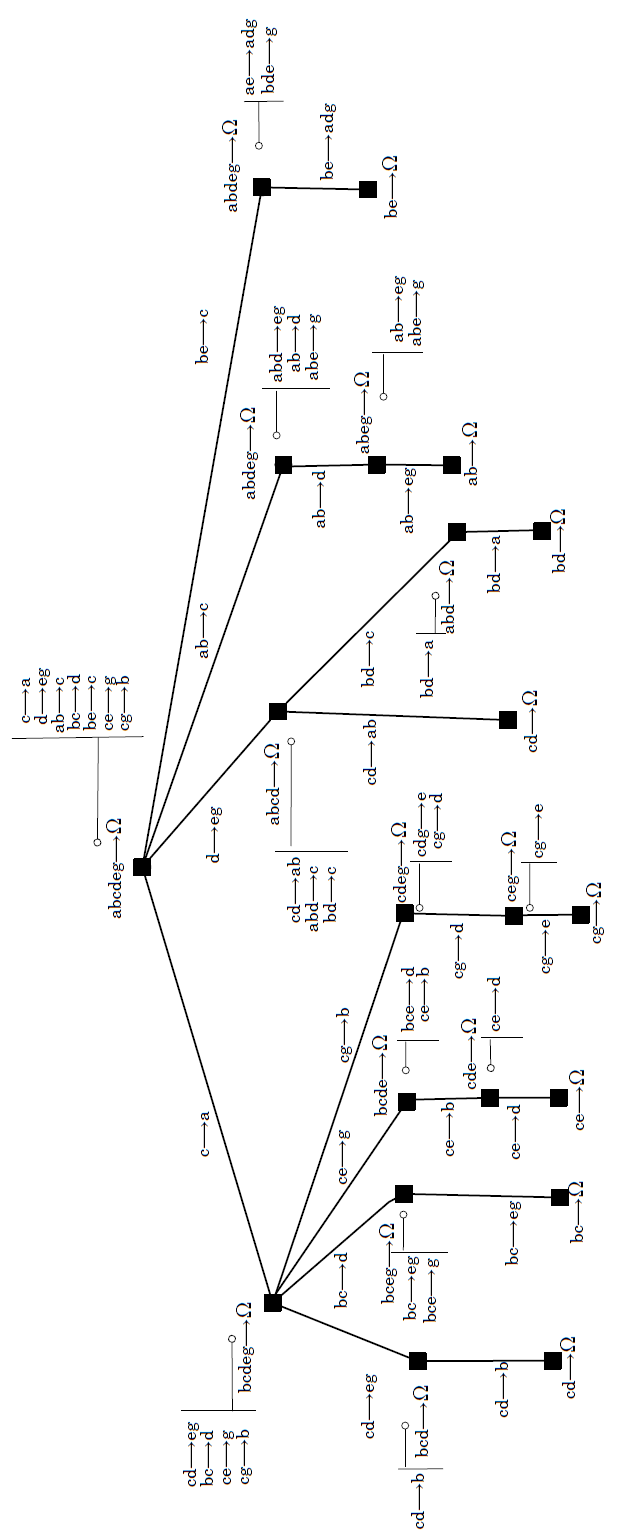
\includegraphics[height=.99\textheight,width=.9\textwidth]{ejemploSLFDMod.png}
	\end{center}
	\caption{Tableaux completo para los datos del ejemplo \ref{ejemploTableauxGrande}.}
	\label{figura:arbolGrande}
\end{figure}
\end{ejemplo}


SST muestra un gran rendimiento en comparaci�n con sus predecesores como hemos visto hasta ahora y como puede comprobarse en el amplio estudio realizado sobre el m�todo en \cite{Benito-Picazo2014TFM}. El beneficio principal en la reducci�n del espacio de b�squeda de debe a la introducci�n del test de inclusi�n para evitar la apertura de ramas extra. Gracias a ello, SST no abre algunas ramas que sabemos que van a producir las mismas claves que se calculan en otra rama. Poder identificar que tales ramas resultar�n en hojas con informaci�n duplicada no es una tema trivial. Para abordarlo, hemos definido la noci�n de implicaci�n minimal con respecto a un conjunto de implicaciones.

\begin{definicion}
Sea $\Gamma$ un conjunto de implicaciones. La implicaci�n $A \to B \in \Gamma$ es minimal si $\forall C \to D \in \Gamma$, se cumple que $C \not\subset A$.
\end{definicion}

Podemos apreciar un ejemplo b�sico de c�mo SST supera a su predecesor en la \slfd, comparando los resultados obtenidos entre las Figuras \ref{figura:arbolSLFD} y \ref{figura:arbolSST}, para \slfde y SST respectivamente.

\begin{figure}
	\centering
		\includegraphics*[width=.99\textwidth,height=.3\textheight]{arbolSLFD.png}
		\caption{M�todo \slfd. Tableaux de 3 niveles. 37 nodos. 18 hojas.}
		\label{figura:arbolSLFD} 
\end{figure}

\begin{figure}
	\centering
		\includegraphics*[width=.99\textwidth,height=.3\textheight]{arbolSLFDMod.png}
		\caption{M�todo SST. Tableaux de 2 niveles. 19 nodos. 12 hojas.}
		\label{figura:arbolSST}
\end{figure}




\subsection*{M�todo CK}
\label{subsec:metodoCK}
El objetivo principal para seguir progresando en esta l�nea es la reducci�n del espacio de b�squeda que se puede cuantificar a trav�s del n�mero de nodos en el �rbol. Con esta intenci�n, hemos estudiado c�mo reducir a�n m�s el tama�o del �rbol al acortar su profundidad. El resultado es este nuevo m�todo \textit{CK} cuyo n�cleo es el algoritmo del cierre l�gico publicado en \cite{Mora2012} y que ya hemos visto como \cierree puede considerarse un novedoso enfoque a los m�todos cl�sicos de cierre, ya que proporciona una nueva caracter�stica: adem�s del conjunto de atributos que constituye la salida del operador de cierre, el m�todo proporciona un subconjunto de implicaciones del conjunto $\Gamma$ original. Este nuevo subconjunto de implicaciones re�ne el conocimiento que puede considerarse como el complemento del cierre y se puede usar de una manera inteligente para encontrar claves minimales por medio del operador de cierre.

La ventaja principal del m�todo es que recibe un conjunto de implicaciones $\Gamma$ y un subconjunto de atributos $X \subseteq \Omega$. Calcula el conjunto cierre $X^+$ respecto a $\Gamma$, y adem�s, un nuevo conjunto $\Gamma^\prime$ que contiene el conjunto de implicaciones que guarda la sem�ntica que queda fuera del cierre $X^+$. Si $\Gamma^\prime = \varnothing$, entonces $X^+ = \Omega$ (v�ase \cite{Mora2012} para m�s detalles).

Por tanto, proponemos aplicar el \cierree a cada implicaci�n minimal del conjunto $\Gamma$ en cada nodo para abrir nuevas ramas con el resultado producido por el cierre \cierre. La definici�n de nuestro nuevo m�todo de claves minimales se presenta en el Algoritmo \ref{algoritmo:CK}.

\begin{algorithm2e}
{\scriptsize
%\DontPrintSemicolon
\KwData{

$\Omega$ un conjunto de atributos.

$\Gamma$ un conjunto de implicaciones.

${\cal C}$ una variable acumuladora con un subconjunto de atributos.

${\mathcal K}$ una variable acumuladora con conjuntos de atributos.}
%\KwResult{${\mathcal K}$, set of all minimal keys.}
\Begin{
        ${\cal A}$ := $\Omega$\\
        %${\mathcal K}:= \varnothing $\\
        \lIf{$\Gamma=\varnothing$}{\\             
        \ \ \ \ Add(${\mathcal K}, \{{\cal A}\cup {\cal C}\})$
            %{\Return ${\cal A}$}
        }\bf else{\\
        \ \ \ \ \ForEach{$X \to Y \in \text{[IM]}(\Gamma)$}{
        	\ \ \ \ $<X^\prime,\Gamma^\prime>$ := \cierre $(X,\Gamma)$\\
          \ \ \ \ ${\cal C}:={\cal C}\cup X$\\
        	\ \ \ \ {\bf Closure\_Keys}($X^\prime,\Gamma^\prime, {\cal C}, {\mathcal K}$)\\
        				}
        }
             %   \Return  ${\scriptsize \tt{Minimal}} (\mathcal K)$\\

        /* Donde [IM]$(\Gamma)$ denota las implicaciones en $\Gamma$ que son minimales. */
}
}
\caption{Closure Keys (CK)}
\label{algoritmo:CK}
\end{algorithm2e}

La llamada principal del Algoritmo \ref{algoritmo:CK} debe ser Closure\_Keys($\Omega,\Gamma,\varnothing,\varnothing$). A continuaci�n, para obtener todas las claves m�nimales, recogemos los elementos minimales del cuarto par�metro (que act�a como un acumulador en modo de entrada/salida) de esta llamada a procedimiento con respecto a $(2^\Omega,\subseteq)$. El siguiente teorema asegura que el Algoritmo \ref{algoritmo:CK} proporciona un m�todo v�lido y completo.

\begin{theorem}\label{ThGordo}
Sea $\Omega$ un conjunto de atributos y $\Gamma$ un sistema de implicaciones sobre $M$. Entonces, el Algoritmo \ref{algoritmo:CK} devuelve todas las claves minimales.
\end{theorem}

\begin{demostracion}
En primer lugar, la terminaci�n del algoritmo est� garantizada porque, en cada llamada recursiva de Closure\_Keys, la cardinalidad del sistema de implicaciones se reduce estrictamente. Adem�s, el n�mero de llamadas recursivas est� limitado por la cardinalidad de $\Gamma$. El n�cleo del m�todo es el cierre \cierre \cite{Mora2012} que proporciona un resultado compuesto, es decir, $\cierre(X,\Gamma)= <X^+, \Gamma^\prime>$.

Este m�todo genera todas las claves minimales porque, en cada paso produce el cierre $X^+$ y si resulta que ese cierre no es el conjunto $\Omega$ completo, procedemos seleccionando un nuevo antecedente del conjunto de implicaciones $\Gamma^\prime$. En virtud de esto, una vez que alcanzamos una hoja, la uni�n de los antecedentes en el camino conforma una clave y por lo tanto, el m�todo es \emph{v�lido}.

Con respecto a la \emph{completitud}, cualquier clave del sistema se va a encontrar ya que el espacio de b�squeda inducido por nuestro m�todo realiza una b�squeda exhaustiva.

\QED
\end{demostracion}

Al igual que en el apartado anterior donde mostramos un ejemplo de comparaci�n entre el �rbol generado por el m�todo \slfde y el m�todo SST (Figura \ref{figura:arbolSLFD} y \ref{figura:arbolSST}, respectivamente), un ejemplo ilustrativo que muestra la reducci�n en el �rbol proporcionado por CK con respecto al m�todo SST se muestra en las figuras \ref{figura:arbolCK} y \ref{figura:arbolSST} respectivamente.

\begin{figure}
	\centering
		\includegraphics*[width=.99\textwidth,height=.4\textheight]{arbolSST.png}
		\caption{Ejemplo completo de aplicaci�n utilizando el m�todo SST.}
		\label{figura:arbolSST} 
\end{figure}

\begin{figure}
	\centering
		\includegraphics*[width=.99\textwidth,height=.25\textheight]{arbolCK.png}
		\caption{Ejemplo completo de aplicaci�n utilizando el m�todo CK donde se aprecia la mejora obtenida por CK sobre SST en cuando a la reducci�n del �rbol de b�squeda, pasando de 21 nodos en SST a 11 con CK.}
		\label{figura:arbolCK}
\end{figure}


\section{Implementaci�n}
\label{seccion:implementacion}
Como conclusi�n de los ejemplos presentados en la secci�n anterior, vemos que incluso para ejemplos b�sicos, el �rbol de b�squeda va alcanzando dimensiones considerables. De hecho, podemos consultar estudios previos donde el m�todo \slfde llega a construir �rboles de millones de nodos \cite{Benito-Picazo2014}. Por tanto, para poder salvar este escollo y utilizar los m�todos sobre grandes cantidades de datos, vamos a utilizar estrategias de paralelismo sobre arquitecturas hardware con altos recursos.

Nuestra intenci�n es aprovechar el dise�o del Tableaux en nuestros m�todos para dividir el problema original en instancias at�micas que pueden resolverse por separado en un tiempo razonable y con los recursos disponibles. El resultado con todas las claves minimales lo obtenemos a partir de unificar los resultados individuales obtenidos para cada una de esas instancias at�micas. 

De esta forma, las implementaciones paralelas de los algoritmos funcionar�n en dos etapas:

\begin{enumerate}
	\item \textbf{C�digo parcial.} Ejecuta el m�todo de b�squeda de claves, en vez de construir el �rbol entero, se detendr� en un cierto nivel determinado seg�n un valor de corte (ver a continuaci�n) generando un conjunto de sub-problemas, uno por nodo del �rbol en ese nivel. El resultado de esta etapa es un conjunto de problemas de b�squeda de claves m�s simples.
	\item \textbf{C�digo paralelo.} En esta segunda etapa, ejecutamos el algoritmo de b�squeda de claves sobre cada uno de los sub-problemas generados en la etapa anterior de forma paralelavy, al final, combinamos todas las soluciones para obtener todas las claves minimales.
\end{enumerate}

La Figura \ref{figura:diagramaParalelo} muestra un esquema conceptual de la estrategia paralela.

\begin{figure}
	\centering
		\includegraphics*[width=.75\textwidth,height=.2\textheight]{diagramaParalelo.png}
		\caption{Esquema del funcionamiento en dos etapas del c�digo paralelo.}
		\label{figura:diagramaParalelo}
\end{figure}

Podemos utilizar este tipo de estrategia \textit{MapReduce} \cite{Dean2004} sobre la implementaci�n paralela porque, debido a la naturaleza del �rbol, cada rama ser� totalmente independiente de otras, por lo que cada nodo puede tratarse de manera independiente. Ese es la gran ventaja de usar el paralelismo para de estas t�cnicas; podemos enviar una gran cantidad de problemas a diferentes n�cleos de computaci�n de manera que pueden ser resueltos simult�neamente. En virtud de esto, el tama�o de los problemas en la entrada puede see mucho mayor de lo que la literatura nos muestra hasta ahora sin exceder las limitaciones de la m�quina; hemos alejado el l�mite de una manera sustancial por el momento.

Como hemos mencionado, mediante la aplicaci�n del c�digo parcial, dividimos el problema de entrada en varios sub-problemas, sin embargo, es necesario aclarar cu�l es el valor que decide ese punto de parada (BOV, en ingl�s, \textit{break-off value}).

\subsection*{Valor de parada}
\label{subseccion:BOV}
Decidir el BOV es una labor crucial de la investigaci�n actual debido a las siguientes consideraciones. Por un lado, si decidimos parar en un nivel cercano a la ra�z del �rbol seleccionando un BOV bajo, ciertamente estamos reduciendo el tiempo de ejecuci�n de la etapa de divisi�n y s�lo se crear�n unos pocos subproblemas. Dado que el �rbol no habr�a podido expandirse todav�a, entonces no contaremos con suficiente material para ser gestionado en paralelo usando diferentes n�cleos. Por otro lado, si detenemos la divisi�n de la etapa parcial llegados a un nivel m�s profundo del �rbol y lejos de la ra�z, la divisi�n seguramente crear� una gran cantidad de subproblemas. Esta situaci�n nos va a permitir resolver esos subproblemas usando m�ltiples n�cleos pero, el tiempo de ejecuci�n de la primera etapa seguramente sea mayor. Por lo tanto, hemos tendio que seleccionar BOV de forma emp�rica, ya que es realmente dif�cil averiguar el valor m�s adecuado simplemente analizando la informaci�n de entrada.

En nuestro caso, como valor de parada que determina el nivel en el que la rama se considera at�mica para ser tratada por la etapa paralela, usamos el cardinal del conjunto de implicaciones del nodo actual, ya que hemos observado que, cuanto mayor es, m�s larga \textit{suele ser} la rama. Sin embargo, en la etapa actual de la investigaci�n, s�lo podemos considerar eso como una tendencia, nunca una certeza.

Una vez que tenemos todos estos subproblemas, y debido a que todos ellos conforman un estado individual del algoritmo, pueden ser resueltos por el c�digo paralelo. Sin embargo, si estamos tratando con problemas con una cantidad considerable de atributos e implicaciones, el n�mero de subproblemas generados podr�a ser enorme (hemos realizado experimentos con m�s de 50,000 subproblemas \cite{Benito-Picazo2014TFM}). Por lo tanto, su gesti�n es una tarea que solo est� al alcance de una gran cantidad de recursos, como los ofrecidos por el Centro de Supercomputaci�n y Bioinnovaci�n de la Universidad de M�laga \footnote{http://www.scbi.uma.es}.



\section{Experimentos y resultados}
\label{seccion:experimentosResultados}
Llegamos a la secci�n donde vamos a mostrar una serie de experimentos y resultados para determinar c�mo los algoritmos estudiados e implementados en la secci�n anterior \ref{sec:metodosSSTCK} tratan con problemas m�s complejos de forma que se aprovechen los beneficios del paralelismo.

Hemos elaborado de forma aleatoria un conjunto de problemas variando la cantidad de atributos e implicaciones. En primer lugar, comenzamos con problemas que contienen 100 implicaciones, cada una de ellas construida a partir de 100 atributos diferentes posibles. Y en segundo lugar, avanzamos un paso m�s, considerando problemas con 150 implicaciones y 150 atributos. Hay que tener en cuenta que estos n�meros van m�s all� de las capacidades de la m�quina, como se ha demostrado en estudios previos de este
trabajo \cite{Cordero2013}, e incluso mejoran sustancialmente los resultados dados en \cite{Benito-Picazo2014}, donde ya se aplicaron t�cnicas paralelas.

Obviamente, ambos m�todos obtienen las mismas claves de forma que se valida experimentalmente el m�todo. Por lo tanto, hemos omitido este par�metro en tablas de resultados para mejorar la legibilidad ya que en gran parte de las ocasiones el conjunto de claves puede llegar a ser considerablemente grande. Ahora bien, para comparar los n�meros alcanzados mediante el uso de SST y de CK, nos centramos en dos par�metros fundamentales, tiempos de ejecuci�n y la cantidad de nodos del �rbol. La elecci�n de estos dos par�metros se debe al siguiente razonamiento.  

Cuando nos planteamos la idea de la comparaci�n de resultados, lo primero que consideramos fueron los tiempos que necesitaba cada uno de los m�todos para obtener los resultados: era lo m�s evidente. No obstante, este par�metro est� �ntimamente ligado a la arquitectura que estemos utilizando para ejecutar el algoritmo, lo cual hace que el resultado dependa en gran medida de los recursos que se est�n utilizando y no tanto de la calidad o eficiencia del propio algoritmo. En este sentido, se oscurec�a la utilidad te�rica de los resultados obtenidos. Esto nos llev� a a�adir como segundo par�metro de la comparaci�n, el n�mero de nodos del �rbol como medida de la dimensi�n alcanzada por el problema. Adem�s, si alguien hiciera otro m�todo, utilizara otro c�digo o empleara recursos hardware diferentes que desembocaran en una mejora
del tiempo, siempre podr�amos atenernos al tama�o del �rbol pudiendo defender si realmente es una mejora en el m�todo o en la ejecuci�n debido a la arquitectura.

El n�mero de nodos siempre ser� el mismo para un experimento individual sin importar la cantidad de veces que realicemos el test, sin embargo, los tiempos de ejecuci�n no coincidir�n exactamente con esta circunstancia; podr�an ser ligeramente diferentes debido a su naturaleza intr�nseca. Las diferencias con respecto al n�mero de nodos mostrar�n c�mo los nuevos m�todos han mejorado el algoritmo reduciendo dr�sticamente la profundidad del �rbol, y en consecuencia, los tiempos de ejecuci�n. Adem�s, hemos incluido una �ltima columna para mostrar el ratio entre el n�mero de nodos y el tiempo de ejecuci�n. Finalmente, cada tiempo de ejecuci�n que se muestra es el fruto de un estudio \textit{a posteriori} de los resultados obtenidos de cada ejecuci�n, de forma que conservamos los m�s fiables \cite{Zobel1998}.

Como hemos mencionado anteriormente, la arquitectura hardware que se ha utilizado para desarrollar cada prueba que se muestra en la tesis se puede visitar en \footnote{http://www.scbi.uma.es}. En particular, hemos desarrollado cada experimento usando 32 nodos cluster SL230, utilizando 32 n�cleos y 64Gb de memoria RAM. Las comunicaciones se realizan a trav�s de una red Infiniband FDR. Durante los experimentos, estos n�cleos est�n reservados s�lo para nuestro uso, de manera que podamos evaluar resultados fiables con respecto a los tiempos de ejecuci�n.

Puede parecer que conseguir mejores resultados con la estrategia paralela descrita es simplemente un problema referente a la cantidad de recursos que tengamos disponibles, sin embargo, esto no es del todo cierto. Si bien es cierto que en la mayor�a de los casos hemos obtenidos mejores resultados gracias a utilizar m�s recursos, algunos experimentos para los que se aument� el n�mero de n�cleos disponibles no alcanzaron las expectativas esperadas en t�rminos de tiempos de ejecuci�n, como se muestra brevemente en la Tabla \ref{table:speedup}. Incrementar el n�mero de n�cleos para favorecer el paralelismo dentro de este tipo de problemas es una cuesti�n en la que a�n queda mucho por investigar.

\begin{table}[htbp]
\scriptsize
	\centering
\caption{Intentos de mejorar los tiempos de ejecuci�n en base a aumentar el n�mero de n�cleos disponibles para la implementaci�n paralela.}
\label{table:speedup}
\begin{tabular}{lrrrrrr}
\hline\noalign{\smallskip}
 & Implicaciones & Attrib & Parada \\
 & 150 & 150 & 140 \\
\noalign{\smallskip}\hline\noalign{\smallskip}
Problema \& M�todo & Parcial$_{t}$(s) & Total$_{t}$(s) & Nodos & Cores & Ratio\\
\noalign{\smallskip}\hline\noalign{\smallskip}
150150-4-\sst & 581 & 885 & 55.211 & 32 & 62\\
150150-4-\sck & 48 & 65 & 25.477 & 32 & 391\\
\noalign{\smallskip}\hline\noalign{\smallskip}
150150-4-\sst & 576 & 880 & 55.211 & 64 & 62\\
150150-4-\sck & 46 & 64 & 25.477 & 64 & 398\\
\noalign{\smallskip}\hline
\end{tabular}
\end{table}

Entrando ya en los experimentos realizados, el primero resuelve una bater�a de problemas con 100 atributos y 100 implicaciones y los resultados podemos verlos en la Tabla \ref{table:bigdataI} que est� formada por dos partes. Una cabecera en la que se indica la configuraci�n del experimento, y un cuerpo principal donde se recogen los valores alcanzados para cada problema por parte de cada m�todo. Este cuerpo principal consta de 6 columnas que desglosamos a continuaci�n:

\begin{enumerate}
	\item Nombre del problema y el m�todo utilizado para resolverlo.
	\item N�mero de subproblemas generados en la etapa primera del algoritmo.
	\item Tiempo transcurrido para la etapa primera.
	\item Tiempo total de ejecuci�n (etapa parcial + etapa paralela).
	\item N�mero de nodos del �rbol.
	\item Ratio entre nodos y tiempo de ejecuci�n.
\end{enumerate}

\begin{table}[htbp]
\scriptsize
	\centering
\caption{M�todos paralelos aplicados a problemas grandes (I)}
\label{table:bigdataI}
\begin{tabular}{lrrrrrr}
\hline\noalign{\smallskip}
 & Attrib & Implicaciones & Parada & Cores & \\
 & 100 & 100 & 90 & 32 &  \\
\noalign{\smallskip}\hline\noalign{\smallskip}
Problema \& M�todo  & Subp & Parcial$_{t}$(s) & Total$_{t}$(s) & Nodos & Ratio\\
\noalign{\smallskip}\hline\noalign{\smallskip}
100100-1-\sst & 14 & 0 & 1 & 33 & 33\\
100100-1-\sck & 0 & 0 & 0 & 15 & 15\\
\noalign{\smallskip}\hline\noalign{\smallskip}
100100-2-\sst & 1.354 & 36 & 105 & 25.621 & 244\\
100100-2-\sck & 212 & 4 & 15 & 12.715 & 847\\
\noalign{\smallskip}\hline\noalign{\smallskip}
100100-3-\sst & 8.602 & 183 & 644 & 192.574 & 299\\
100100-3-\sck & 1.286 & 37 & 99 & 94.255 & 952\\
\noalign{\smallskip}\hline\noalign{\smallskip}
100100-4-\sst & 400 & 7 & 26 & 1.704 & 65\\
100100-4-\sck & 15 & 1 & 2 & 751 & 375\\
\noalign{\smallskip}\hline\noalign{\smallskip}
100100-5-\sst & 39 & 0 & 2 & 119 & 59\\
100100-5-\sck & 0 & 0 & 1 & 42 & 42\\
\noalign{\smallskip}\hline\noalign{\smallskip}
100100-6-\sst & 1.808 & 37 & 123 & 7.856 & 63\\
100100-6-\sck & 115 & 4 & 9 & 3.698 & 410\\
\noalign{\smallskip}\hline\noalign{\smallskip}
100100-7-\sst & 6.167 & 182 & 489 & 275.429 & 563\\
100100-7-\sck & 1.378 & 24 & 90 & 118.884 & 1.320\\
\noalign{\smallskip}\hline\noalign{\smallskip}
100100-8-\sst & 5.104 & 146 & 415 & 182.167 & 438\\
100100-8-\sck & 1.014 & 19 & 68 & 81.632 & 1.200\\
\noalign{\smallskip}\hline\noalign{\smallskip}
100100-9-\sst & 314 & 11 & 25 & 868 & 34\\
100100-9-\sck & 0 & 1 & 1 & 341 & 341\\
\noalign{\smallskip}\hline\noalign{\smallskip}
100100-10-\sst & 1.130 & 27 & 84 & 12.541 & 149\\
100100-10-\sck & 136 & 4 & 10 & 6.128 & 612\\
\noalign{\smallskip}
\hline
\end{tabular}
\end{table}

Incluso para una cantidad tan grande de atributos y dependencias, s�lo han sido necesarios alrededor de 10 minutos para que el algoritmo m�s lento finalice (problema 100100-3). Adem�s, el tama�o m�ximo alcanzado del �rbol (problema 100100-7) ronda los 300k nodos. Ser�a totalmente descabellado pensar en resolver estos problemas usando
versiones secuenciales de los algoritmos, ya que los tiempos de ejecuci�n se ir�an de las manos. No obstante, estos son resultados son altamente alentadores ya que hubiera sido impensable tratar de reproducir estos experimentos con los m�todos previos \cite{Benito-Picazo2014}. Por tanto, es evidente c�mo el paralelismo es una opci�n muy acertada para abordar este tipo de problemas.

Se obtienen resultados especialmente notables como son los problemas 100100-\{1,5,9\}. En estos casos, hay que notar que CK no crea ning�n subproblema. Por ello, la mejora que se produce es doble: 
\begin{enumerate}
	\item En algunos casos, con el mismo valor de parada, el nuevo m�todo ni siquiera necesita avanzar en la implementaci�n paralela, la parcial es suficiente para resolver estos problemas.
	\item Para aprovechar esta circunstancia, llegado el caso en el que tengamos que trabajar con problemas a�n m�s complejos, podemos establecer un valor de parada m�s cercano a la ra�z del �rbol de forma que el tiempo parcial se reducir� significativamente.
\end{enumerate}

Para el segundo experimento, seguimos la misma l�nea que el anterior y desarrollamos una nueva bater�a de 10 problemas, aumentando esta vez el n�mero de implicaciones y atributos disponibles hasta 150. Cuanto mayor es la complejidad de estos problemas, mayor es la mejora lograda por el nuevo m�todo CK. Los tiempos de ejecuci�n y la cantidad de nodos han sido dr�sticamente reducido como se muestra en la Tabla \ref{table:bigdataII}. Esta vez, decidimos agregar un experimento adicional (problema 150150-EXTRA) debido a los notables resultados que alcanz�.

\begin{table}[htbp]
\scriptsize
	\centering
\caption{M�todos paralelos aplicados a problemas grandes (II)}
\label{table:bigdataII}
\begin{tabular}{lrrrrrr}
\hline\noalign{\smallskip}
 & Attrib & Implicaciones & Parada & Cores & \\
 & 150 & 150 & 140 & 32 &  \\
\noalign{\smallskip}\hline\noalign{\smallskip}
Problema \& M�todo  & Subp & Parcial$_{t}$(s) & Total$_{t}$(s) & Nodos & Ratio\\
\noalign{\smallskip}\hline\noalign{\smallskip}
150150-1-\sst  & 165 & 6 & 14 & 911 & 65 \\
150150-1-\sck & 11 & 2 & 3 & 374 & 124\\
\noalign{\smallskip}\hline\noalign{\smallskip}
150150-2-\sst & 2.949 & 229 & 394 & 116.517 & 295\\
150150-2-\sck & 347 & 25 & 44 & 54.375 & 1.235\\
\noalign{\smallskip}\hline\noalign{\smallskip}
150150-3-\sst & 12.968 & 1.049 & 1.716 & 157.947 & 92\\
150150-3-\sck & 822 & 125 & 165 & 68.531 & 415\\
\noalign{\smallskip}\hline\noalign{\smallskip}
150150-4-\sst & 5.352 & 581 & 885 & 55.211 & 62\\
150150-4-\sck & 344 & 48 & 65 & 25.477 & 391\\
\noalign{\smallskip}\hline\noalign{\smallskip}
150150-5-\sst & 5.361 & 211 & 484 & 32.377 & 66 \\
150150-5-\sck & 168 & 27 & 36 & 12.522 & 347\\
\noalign{\smallskip}\hline\noalign{\smallskip}
150150-6-\sst & 771 & 72 & 155 & 17.298 & 111\\
150150-6-\sck & 79 & 7 & 11 & 8.110 & 737 \\
\noalign{\smallskip}\hline\noalign{\smallskip}
150150-7-\sst & 9.473 & 638 & 1.252 & 576.912 & 460 \\
150150-7-\sck & 1.754 & 97 & 187 & 262.621 & 1.404 \\
\noalign{\smallskip}\hline\noalign{\smallskip}
150150-8-\sst & 5.466 & 424 & 857 & 510.627 & 595 \\
150150-8-\sck & 966 & 57 & 104 & 257.267 & 2.473 \\
\noalign{\smallskip}\hline\noalign{\smallskip}
150150-9-\sst & 235 & 25 &  45 & 3.632 & 80\\
150150-9-\sck & 24 & 3 & 4 & 1.726 & 431\\
\noalign{\smallskip}\hline\noalign{\smallskip}
150150-10-\sst & 3.403 & 348 & 555 & 102.537 & 184\\
150150-10-\sck & 277 & 31 & 46 & 45.962 & 999 \\
\noalign{\smallskip}\hline\noalign{\smallskip}
150150-EXTRA-\sst & 31.401 & 2.950 & 30.983 & 21.404.732 & 690 \\
150150-EXTRA-\sck & 8.049 & 354  & 1.320 & 10.614.386 & 8.041 \\
\noalign{\smallskip}
\hline
\end{tabular}
\end{table}

Igual que en el caso anterior,  hay varios experimentos que merecen ser discutidos por separado. Por ejemplo, si fijamos nuestra atenci�n en los problemas 150150-\{3,7\}, el n�mero de subproblemas generados es mucho menor para el m�todo CK que para SST. La diferencia, que no es ni mucho menos trivial, tambi�n propicia la gran reducci�n de los tiempos de ejecuci�n de la etapa parcial. Los tiempos totales de ejecuci�n van en la misma direcci�n. En cuanto al tama�o del �rbol, los beneficios al introducir el cierre son bastante llamativos; en la mayor�a de los casos, la cantidad de nodos se reduce en torno al 50\%. Podemos apreciar las diferencias y las mejoras obtenidas m�s c�modamente de forma gr�fica en las Figuras \ref{figura:bigSizeIITiempos} y \ref{figura:bigSizeIINodos}.

\begin{figure}
	\centering
		\includegraphics*[width=.8\textwidth,height=.4\textheight]{totalTimesGraphics.png}
		\caption{Tiempos de ejecuci�n de los m�todos paralelos aplicados a problemas grandes (II).}
		\label{figura:bigSizeIITiempos}
\end{figure}

\begin{figure}
	\centering
		\includegraphics*[width=.8\textwidth,height=.4\textheight]{nodesGraphics.png}
		\caption{Tiempos de ejecuci�n de los m�todos paralelos aplicados a problemas grandes (II).}
		\label{figura:bigSizeIINodos}
\end{figure}


% =====================================================================
% =====================================================================
% =====================================================================
\clearemptydoublepage

% this file is called up by thesis.tex
% content in this file will be fed into the main document
\pagestyle{empty}
%: ----------------------- name of chapter  -------------------------
\chapter{Generadores Minimales}
\label{cap:generadoresMinimales} % top level followed by section, subsection

%: ----------------------- paths to graphics ------------------------

% change according to folder and file names
%\ifpdf
%    \graphicspath{{X/figures/PNG/}{X/figures/PDF/}{X/figures/}}
%\else
%   \graphicspath{{X/figures/EPS/}{X/figures/}}
%\fi

%: ----------------------- contents from here ------------------------


\pagestyle{headings}

\bigdrop{0pt}{5}{cmr10}El sistema de inferencia de \slfde \cite{Enciso2002,Cordero2012} y la salida del algoritmo \cierree se pueden usar para enumerar todos los conjuntos cerrados y todos los generadores minimales a partir de un conjunto de implicaciones y de atributos. Por tanto, el contenido de este cap�tulo va a estar muy ligado al anterior y muchos de los conceptos van a aparecer nuevamente.

En el cap�tulo de introducci�n \ref{cap:introduccion} habl�bamos de dos formas de representaci�n del conocimiento: los sistemas de implicaciones y los ret�culos de conceptos. Asimismo, vimos que existen varios problemas y soluciones en cuanto a extraer ambas representaciones a partir de un \textit{dataset} de entrada. Sin embargo, en este momento vamos a tratar con un problema complementario que permite conectar ambas representaciones del conocimiento: la enumeraci�n de todas los conjuntos cerrados de un conjunto dado de implicaciones. Adem�s, proponemos un m�todo para producir no s�lo todos los conjuntos cerrados, sino tambi�n, para cada uno de ellos, su representante can�nico, denominados generadores minimales.

La importancia de los generadores m�nimos est� bien justificada por trabajos notables como el profundo estudio de Poelmans et al. \cite{Poelmans2013} o el de Qu et al. \cite{Qu2007}. Por otra parte, han sido utilizados como punto fundamental para construir bases, las cuales constituyen una representaci�n compacta del conocimiento que permite un mejor rendimiento de los m�todos de razonamiento basados en reglas \cite{Missaoui2010,Missaoui2012}. Todos los autores mencionados han considerado el \textit{dataset} como la entrada del problema, es decir, los generadores minimales y los conjuntos cerrados se infieren a partir de la informaci�n original. En \cite{Hamrouni2007,Nishio2012a} se proponen algunos m�todos para resolver este problema.

En nuestro caso, centr�ndonos una vez m�s en el tratamiento inteligente de los conjuntos de implicaciones, vamos a utilizarlas como los elementos para describir la informaci�n y adem�s, como base del dise�o de un m�todo para enumerar todos los conjuntos cerrados y sus generadores minimales a partir de esta informaci�n, y no del \textit{dataset} original (como en los trabajos mencionados), lo cual, hasta donde sabemos, no existe trabajo previo al respecto. El nuevo m�todo propuesto utiliza la \slfde y es una evoluci�n de \cite{Cordero2012}. Este m�todo trabaja sobre el conjunto de implicaciones aplicando unas reglas de inferencia y construyendo un espacio de b�squeda de �rbol, lo cual como ya adelantamos al principio del cap�tulo, va a ser muy parecido a los �rboles del caso de las claves minimales.

La generaci�n del sistema de implicaciones asociado a un operador de cierre es un problema dif�cil y el inverso tambi�n, teniendo una complejidad exponencial. Por lo tanto, nos vamos a enfocar en la definici�n de un m�todo para resolver este problema y en el dise�o de una implementaci�n m�s eficiente, particularmente acerc�ndonos al problema utilizando computaci�n paralela.

Por tanto, en este cap�tulo, tras una relacionar brevemente las implicaciones con los generadores minimales \ref{seccion:implicacionesGeneradoresMinimales}, pasaremos a una secci�n fundamental donde se exponen cada uno de los m�todos analizados e implementados \ref{seccion:metodosGeneradoresMinimales}. Para cada uno de ellos se presenta su definici�n en forma de algoritmo y se acompa�a de un ejemplo ilustrativo de su funcionamiento. Una vez presentados los m�todos, en la secci�n \ref{seccion:resultadosGeneradoresMinimales} se presenta de forma m�s detallada los pruebas realizadas y los resultados obtenidos por cada m�todo. De forma similar a lo que se present� para el cap�tulo de claves, cerrar�n el cap�tulo los experimentos y los resultados obtenidos, esta vez, sobre la arquitectura de computaci�n paralela \ref{seccion:computacionParalelaGeneradoresMinimales}.


\section{Implicaciones y generadores minimales}
\label{seccion:implicacionesGeneradoresMinimales}
Se dice que un sistema de implicaciones es completo para un operador de cierre si captura todo el conocimiento relacionado con ese operador (contexto), es decir, el sistema de implicaciones expresa en el lenguaje de la l�gica todo el conocimiento relativo al cierre. Formalmente:

\begin{definicion}
Sea $c\colon 2^M\to 2^M$ un operador de cierre sobre $M$ y $\Sigma\subseteq \mathcal L_M$. El sistema de implicaciones $\Sigma$ se dice que es completo para $c$ si se verifica la siguiente equivalencia:
$$
\forall A\to B\in\mathcal L_M, \quad c\models A\to B\quad\text{si y s�lo si }\quad \Sigma\models A\to B
$$
\end{definicion}


De forma inmediata, cuando un sistema de implicaciones $\Sigma$ es completo para un operador de cierre $c$, su operador de cierre sint�ctico coincide con $c$, es decir, $X^+_\Sigma = c(X) \ \ \forall X\subseteq M$.

Como hemos mostrado, cualquier operador de cierre $c$ en $M$ puede asociarse con un sistema de implicaciones. Esta conexi�n establece una forma de gestionar el trabajo del operador de cierre $c$ por medio de su derivaci�n sint�ctica y, como consecuencia, se puede elaborar un m�todo para realizar esta gesti�n. Pero, �qu� pasa con la conexi�n inversa? Es decir, dado un conjunto de implicaciones, �es posible generar el operador de cierre $c$ asociado a �l? Tal pregunta es el n�cleo de esta parte de la tesis y su soluci�n implica enumerar todos los conjuntos cerrados.

Si tenemos que $X,Y \subseteq M$ satisfacen que $X = Y^+_\Sigma$, es habitual decir que $Y$ es un generador del conjunto cerrado $X$. Observe que cualquier subconjunto de $X$ que contiene $Y$ es tambi�n un generador de $X$. Dado que trabajamos con conjuntos finitos de atributos, el conjunto de los generadores de un conjunto cerrado se pueden caracterizar por sus generadores minimales.

\begin{definicion}[Generador minimal]
Sea $c\colon 2^M\to 2^M$ un operador de cierre, sea $C \subseteq M$ un conjunto cerrado, i.e. $c(C) = C$, y sea $A\subseteq M$. El conjunto $A$ se denomina generador minimal (en adelante, \textit{mingen}) para $C$ con respecto a $c$ si $c(A) = C$ y, $\forall X\subseteq A$, si $c(X) = C$, entonces $X = A$.  
\end{definicion}


\section{M�todos para calcular los generadores minimales}
\label{seccion:metodosGeneradoresMinimales}
En \cite{Cordero2012}, se utiliz� la \slfde como herramienta para encontrar todos los generadores minimales a partir de un conjunto de implicaciones. El m�todo emplea la funci�n \ref{algoritmo:Cls} para guiar la b�squeda de nuevos candidatos de generador minimal. Concretamente, dado un conjunto de atributos $M$ y un sistema de implicaciones $\Sigma$, el m�todo realiza un mapeo $mg_\Sigma\colon 2^M\to 2^{2^M}$ que satisface la siguiente condici�n.

$$\forall X,Y\subseteq M$$

\begin{center}
$X\in mg_\Sigma(C)$ si y s�lo si $C$ es cerrado para $(\ )^+_\Sigma$ y $X$ es un generador minimal para $C$.
\end{center}

\begin{ejemplo}
Sea $\Sigma=\{a\to c, bc\to d, c\to ae, d\to e\}$, el mapeo $mg_\Sigma$ se describe como:
\begin{center}
\begin{tabular}{p{1.6cm}|p{.4cm}p{.3cm}p{.3cm}p{.5cm}p{.5cm}p{.6cm}p{.6cm}p{.8cm}p{.9cm}}
$X$ & $\varnothing$ & $b$ & $e$ & $be$ & $de$ & $ace$ & $bde$ &  $acde$ &   $abcde$   \\
\hline
$mg_\Sigma(X)$ &$\varnothing$ & $b$ & $e$ & $be$ & $d$  & $a$ & $bd$ & $ad$ & $ab$ 
\\
& & & & & & $c$& &$cd$ & $bc$    
\end{tabular}
\end{center}

En otro caso, $X$ no es cerrado y $mg_\Sigma(X)=\varnothing$. N�tese que $\varnothing$ es cerrado y $mg_{\Sigma}(\varnothing)=\{\varnothing\}$, i.e. $\varnothing$ es un generador minimal del conjunto cerrado $\varnothing$.
\end{ejemplo}

Los algoritmos que presentamos en esta secci�n deben usar la siguiente operaci�n para este tipo de mapeos. Dados dos mapeos: $mg_1,mg_2\colon 2^M\to 2^{2^M}$, el mapeo $mg_1\sqcup mg_2\colon 2^M\to 2^{2^M}$ se define como:

$$(mg_1\sqcup mg_2)(X)={\tt Minimals}(mg_1(X)\cup mg_2(X)) \ \ \forall X\subseteq M$$

Por tanto, $Y\in (mg_1\sqcup mg_2)(X)$ sii $Y$ es un conjunto minimal de $mg_1(X)\cup mg_2(X)$ en $(2^M,\subseteq)$, i.e. $Y\in mg_1(X)\cup mg_2(X)$ y no existe otro conjunto de atributos $Z\in mg_1(X)\cup mg_2(X)$ tal que $Z\varsubsetneq Y$.

Finalmente, con lo mostrado en esta secci�n, ya tenemos todas las herramientas necesarias para definir el m�todo \textit{Minimal Generator}.

\subsection{M�todo MinGen}
El primer m�todo de c�lculo de los generadores minimales que hemos estudiado e implementado se introdujo originalmente en \cite{Cordero2012}. En nuestro caso, para la tesis lo describimos seg�n la funci�n \ref{algoritmo:minGen} y lo acompa�amos de un ejemplo de aplicaci�n en \ref{ejemplo:minGenBasico} 

\begin{function}[h]
\caption{MinGen($M$, Label, Guide, $\Sigma$)}
\label{algoritmo:minGen}
\small
\DontPrintSemicolon
\SetKwInOut{Input}{input}
\SetKwInOut{Output}{output}
\Input{Conjunto de atributos $M$. \\
Un conjunto auxiliar para construir un generador minimal, Label.\\
Un conjunto auxiliar para construir un conjunto cerrado, Guide.\\ 
Un sistema de implicaciones $\Sigma$ en $M$.}
\Output{El mapeo $mg_\Sigma$.}
\Begin{
	\ForEach{$X\subseteq M$}{
	
		\ \ $mg_\Sigma(X) := \varnothing$
	}
	\vspace{0.2cm}
	(Guide, $\Sigma$) := {\tt Cls}(Guide, $\Sigma$)
	
	$M := M\smallsetminus$Guide
	
	\vspace{0.2cm}
	$\mathrm{Premises} := \{A\subseteq M\mid  A\to B\in \Sigma\text{ for some }B\subseteq M\}$
	ClosedSets$:=\{X\subseteq M\mid A\not\subseteq X \text{ for all }A\in \mathrm{Premises}\}$

	\vspace{0.2cm}
	\ForEach{$X\in \mathrm{ClosedSets}$}{
	
		\ \ $mg_\Sigma(\mathrm{Guide}\cup X) := \{\mathrm{Label}\cup X\}$
	}
	
	\vspace{0.2cm}
	\ForEach{$A\in \mathrm{Premises}$}{
	
		$mg_\Sigma := mg_\Sigma\sqcup\mathrm{MinGen}(M, \mathrm{Label}\cup A, \mathrm{Guide}\cup A, \Sigma)$
	}
	\Return $mg_\Sigma$
}
\end{function}

La entrada de MinGen es un subconjunto de atributos de $M$ y un conjunto de implicaciones $\Sigma$. El resultado es el conjunto de conjuntos cerrados junto con todos los generadores minimlaes que los generan, es decir, $\{\langle C, mg_\Sigma(C)\rangle: C$ es un conjunto cerrado\} donde $mg_\Sigma(C)$ es el conjunto de generadores minimales $D$ que satisfacen $D^+_\Sigma = C$.

\begin{ejemplo}
\label{ejemplo:minGenBasico}
Sea el sistema de implicaciones $\Sigma = \{a\to c, bc\to d, c\to ae, d\to e\}$. La funci�n \ref{algoritmo:minGen}$(abcde,\varnothing,\varnothing,\Sigma)$ devuelve el siguiente resultado:  
\begin{center}
\begin{tabular}{p{1.6cm}|p{.4cm}p{.3cm}p{.3cm}p{.5cm}p{.6cm}p{.8cm}p{.9cm}p{.6cm}p{.8cm}}
$X$ & $\varnothing$ & $b$ & $e$ & $be$& $ace$ &  $acde$ &   $abcde$ & $de$ & $bde$  \\
\hline
$mg_\Sigma(X)$ &$\varnothing$ & $b$ & $e$ & $be$& $a$ & $ad$ & $ab$ & $d$ & $bd$ 
\\
& & &  & & $c$ &$cd$ & $bc$&  &  
\end{tabular}
\end{center}

El �rbol de b�squeda que se va generando lo podemos ver en la Figura \ref{figura:arbolMinGenEjemplo} y la traza de ejecuci�n la mostramos a continuaci�n.

\begin{figure}[htbp]
	\begin{center}
		\includegraphics*[width=.95\textwidth,height=.27\textheight]{arbolMinGenEjemplo.png}
	\end{center}
	\caption{�rbol de b�squeda que genera el algoritmo \ref{algoritmo:minGen} para el Ejemplo \ref{ejemplo:minGenBasico}.}
	\label{figura:arbolMinGenEjemplo}
\end{figure}

MinGen$(abcde,\varnothing,\varnothing,\{a\to c, bc\to d, c\to ae, d\to e\})$:
\begin{center}
Cls$(\varnothing,\Sigma)=(\varnothing,\{a\to c, bc\to d, c\to ae, d\to e\})$ y

\begin{tabular}{p{1.6cm}|p{.4cm}p{.3cm}p{.3cm}p{.5cm}}
$X$ & $\varnothing$ & $b$ & $e$ & $be$ \\
\hline
$mg_\Sigma(X)$ &$\varnothing$ & $b$ & $e$ & $be$
\end{tabular}
\end{center}
\begin{enumerate}
\item[1] MinGen$(abcde,a,a,\{a\to c, bc\to d, c\to ae, d\to e\})$:
\begin{center}
Cls$(a,\{a\to c, bc\to d, c\to ae, d\to e\})=(ace,\{ b\to d\})$ y

\begin{tabular}{p{1.6cm}|p{.6cm}p{.6cm}}
$X$ & $ace$ & $acde$ \\
\hline
$mg_{\Sigma_1}(X)$ & $a$ & $ad$
\end{tabular}
\end{center}
\begin{enumerate}
\item[1.1] MinGen$(bd,ab,abce,\{b\to d\})$:
\begin{center}
Cls$(abce,\{b\to d\})=(abcde,\varnothing)$ y

\begin{tabular}{p{1.8cm}|p{.8cm}}
$X$ &  $abcde$ \\
\hline
$mg_{\Sigma_{1.1}}(X)$ & $ab$
\end{tabular}
\end{center}
\end{enumerate}
Volvemos al nivel 1: $mg_{\Sigma_1}:=mg_{\Sigma_1}\sqcup mg_{\Sigma_{1.1}}$ y entonces
\begin{center}
\begin{tabular}{p{1.6cm}|p{.6cm}p{.7cm}p{.8cm}}
$X$ & $ace$ & $acde$ &  $abcde$ \\
\hline
$mg_{\Sigma_1}(X)$ & $a$ & $ad$ & $ab$
\end{tabular}
\end{center}

\end{enumerate}
Volvemos al nivel raiz: $mg_{\Sigma}:=mg_{\Sigma}\sqcup mg_{\Sigma_{1}}$ y 
\begin{center}
\begin{tabular}{p{1.6cm}|p{.4cm}p{.3cm}p{.3cm}p{.5cm}p{.6cm}p{.7cm}p{.8cm}}
$X$ & $\varnothing$ & $b$ & $e$ & $be$& $ace$ & $acde$ &  $abcde$ \\
\hline
$mg_\Sigma(X)$ &$\varnothing$ & $b$ & $e$ & $be$& $a$ & $ad$ & $ab$
\end{tabular}
\end{center}
\begin{enumerate}
\item[2] MinGen$(abcde,bc,bc,\{a\to c, bc\to d, c\to ae, d\to e\})$:
\begin{center}
Cls$(bc,\{a\to c, bc\to d, c\to ae, d\to e\})=(abcde,\varnothing)$

\begin{tabular}{p{1.6cm}|p{.8cm}}
$X$ & $abcde$ \\
\hline
$mg_{\Sigma_2}(X)$ & $bc$
\end{tabular}
\end{center}
\end{enumerate}
Volvemos al nivel raiz: $mg_{\Sigma}:=mg_{\Sigma}\sqcup mg_{\Sigma_{2}}$ y 
\begin{center}
\begin{tabular}{p{1.6cm}|p{.4cm}p{.3cm}p{.3cm}p{.5cm}p{.6cm}p{.8cm}p{.8cm}}
$X$ & $\varnothing$ & $b$ & $e$ & $be$& $ace$ & $acde$ &  $abcde$ \\
\hline
$mg_\Sigma(X)$ &$\varnothing$ & $b$ & $e$ & $be$& $a$ & $ad$ & $ab$
\\
& & &  & &  & & $bc$
\end{tabular}
\end{center}
%=====

\begin{enumerate}
\item[3] MinGen$(abcde,c,c,\{a\to c, bc\to d, c\to ae, d\to e\})$:
\begin{center}
Cls$(c,\{a\to c, bc\to d, c\to ae, d\to e\})=(ace,\{ b\to d \})$ anyd

\begin{tabular}{p{1.6cm}|p{.6cm}p{.6cm}}
$X$ & $ace$ & $acde$ \\
\hline
$mg_{\Sigma_3}(X)$ & $c$ & $cd$
\end{tabular}
\end{center}
\begin{enumerate}
\item[3.1] MinGen$(bd,bc,abce,\{b\to d\})$:
\begin{center}
Cls$(abce,\{b\to d\})=(abcde,\varnothing)$ y

\begin{tabular}{p{1.8cm}|p{.8cm}}
$X$ &  $abcde$ \\
\hline
$mg_{\Sigma_{3.1}}(X)$ & $bc$
\end{tabular}
\end{center}
\end{enumerate}
Volvemos al nivel 3: $mg_{\Sigma_3}:=mg_{\Sigma_3}\sqcup mg_{\Sigma_{3.1}}$ y entonces
\begin{center}
\begin{tabular}{p{1.6cm}|p{.6cm}p{.8cm}p{.8cm}}
$X$ & $ace$ & $acde$ &  $abcde$\\
\hline
$mg_{\Sigma_3}(X)$ & $c$ & $cd$& $bc$
\end{tabular}
\end{center}
\end{enumerate}
Volvemos al nivel raiz: $mg_{\Sigma}:=mg_{\Sigma}\sqcup mg_{\Sigma_{3}}$ y 
\begin{center}
\begin{tabular}{p{1.6cm}|p{.4cm}p{.3cm}p{.3cm}p{.5cm}p{.6cm}p{.8cm}p{.9cm}}
$X$ & $\varnothing$ & $b$ & $e$ & $be$& $ace$ &  $acde$ &   $abcde$   \\
\hline
$mg_\Sigma(X)$ &$\varnothing$ & $b$ & $e$ & $be$& $a$ & $ad$ & $ab$ 
\\
& & &  & & $c$ &$cd$ & $bc$
\end{tabular}
\end{center}

%=====
\begin{enumerate}
\item[4] MinGen$(abcde,d,d,\{a\to c, bc\to d, c\to ae, d\to e\})$:

\begin{center}
Cls$(d,\{a\to c, bc\to d, c\to ae, d\to e\})=(de,\{a\to c, c\to a\})$ y

\begin{tabular}{p{1.6cm}|p{.6cm}p{.6cm}}
$X$ & $de$ & $bde$ \\
\hline
$mg_{\Sigma_4}(X)$ & $d$ & $bd$
\end{tabular}
\end{center}
\begin{enumerate}
\item[4.1] MinGen$(abc,ad,ade,\{a\to c, c\to a\})$:

\begin{center}
Cls$(ade,\{a\to c, c\to a\})=(acde,\varnothing)$ y

\begin{tabular}{p{1.8cm}|p{.8cm}p{.8cm}}
$X$ &  $acde$&  $abcde$ \\
\hline
$mg_{\Sigma_{4.1}}(X)$ & $ad$& $abd$
\end{tabular}
\end{center}
\end{enumerate}
Volvemos al nivel 4: $mg_{\Sigma_4}:=mg_{\Sigma_4}\sqcup mg_{\Sigma_{4.1}}$ y entonces
\begin{center}
\begin{tabular}{p{1.6cm}|p{.6cm}p{.6cm}p{.8cm}p{.8cm}}
$X$ & $de$ & $bde$ &  $acde$&  $abcde$ \\
\hline
$mg_{\Sigma_4}(X)$ & $d$ & $bd$ & $ad$& $abd$
\end{tabular}
\end{center}
\begin{enumerate}
\item[4.2] MinGen$(abc,cd,cde,\{a\to c, c\to a\})$:
\begin{center}
Cls$(cde,\{a\to c, c\to a\})=(acde,\varnothing)$ y

\begin{tabular}{p{1.8cm}|p{.8cm}p{.8cm}}
$X$ &  $acde$&  $abcde$ \\
\hline
$mg_{\Sigma_{4.2}}(X)$ & $cd$& $cbd$
\end{tabular}
\end{center}
\end{enumerate}
Volvemos al nivel 4: $mg_{\Sigma_4}:=mg_{\Sigma_4}\sqcup mg_{\Sigma_{4.2}}$ y entonces
\begin{center}
\begin{tabular}{p{1.6cm}|p{.5cm}p{.6cm}p{.8cm}p{.8cm}}
$X$ & $de$ & $bde$ &  $acde$&  $abcde$ \\
\hline
$mg_{\Sigma_4}(X)$ & $d$ & $bd$ & $ad$& $abd$ 
\\
 &  & & $cd$& $cbd$ 
\end{tabular}
\end{center}
\end{enumerate}
Volvemos al nivel raiz: $mg_{\Sigma}:=mg_{\Sigma}\sqcup mg_{\Sigma_{4}}$ y efectivamente, obtenemos el resultado que hab�amos adelantado
\begin{center}
\begin{tabular}{p{1.6cm}|p{.4cm}p{.3cm}p{.3cm}p{.5cm}p{.6cm}p{.8cm}p{.9cm}p{.6cm}p{.8cm}}
$X$ & $\varnothing$ & $b$ & $e$ & $be$& $ace$ &  $acde$ &   $abcde$ & $de$ & $bde$  \\
\hline
$mg_\Sigma(X)$ &$\varnothing$ & $b$ & $e$ & $be$& $a$ & $ad$ & $ab$ & $d$ & $bd$ 
\\
& & &  & & $c$ &$cd$ & $bc$&  &  
\end{tabular}
\end{center}
\end{ejemplo}

\begin{ejemplo}
\label{ejemplo:minGenGrande}
Sea el conjunto de atributos $M = \{1, 2, 3, 4, 5\}$ y sea el sistema de implicaciones $\Sigma = \{5\to 4, 2\ 3\to 4, 2\ 4\to 3, 3\ 4\to 2, 1\ 4\to 2\ 3\ 5, 2\ 5\to 1\ 3\ 4, 3\ 5\to 1\ 2\ 4, 1\ 5\to 2\ 4, 1\ 2\ 3\to 4\ 5\}$. La funci�n \ref{algoritmo:minGen}$(M,\varnothing,\varnothing,\Sigma)$ genera el �rbol de b�squeda que muestra la Figura \ref{figura:arbolMinGenEjemploGrande} en el que los generadores minimales obtenidos est�n sombreados en color gris.  

\begin{figure}[htbp]
	\begin{center}
		\includegraphics*[width=1\textwidth,height=.7\textheight]{arbolMinGenEjemploGrande.png}
	\end{center}
	\caption{�rbol de b�squeda que genera el algoritmo \ref{algoritmo:minGen} para el Ejemplo \ref{ejemplo:minGenGrande}.}
	\label{figura:arbolMinGenEjemploGrande}
\end{figure}
\end{ejemplo}

El punto clave del algoritmo MinGen recae en el uso del cierre \cierree ya que utiliza las ventajas de la informaci�n adicional que proporciona, es decir, \cierree se usa no s�lo para calcular generadores de conjuntos cerrados sino tambi�n conjuntos de implicaciones m�s peque�os que nos gu�an en la b�squeda de nuevos subconjuntos que resulten en generadores minimales.



\subsection{M�todo MinGenPr}
En esta secci�n presentamos una variante m�s avanzada del m�todo MinGen anterior. Para ello, hemos incorporado un mecanismo de poda para evitar la generaci�n de generadores minimales y cierres redundantes. El prop�sito de esta poda es verificar la informaci�n de cada nodo en el espacio de b�squeda, evitando la apertura de una rama completa. Esta reducci�n s�lo puede llevarse a cabo si podemos garantizar que toda la informaci�n relativa a los generaciones minimales se genera en otras ramas. En la funci�n \ref{algoritmo:minGenPr} esta estrategia de poda se implementa en la l�nea n�mero \#1. Por lo tanto, para garantizar que la informaci�n generada en una rama sea sup�rflua, dise�amos una poda basada en el test de inclusi�n de conjuntos que involucra a todos los nodos del mismo nivel. En la Figura 2, se ilustra c�mo funciona esta estrategia de poda aplicada al siguiente ejemplo:

\begin{function}[h]
\caption{MinGenPr($M$, Label, Guide, $\Sigma$)}
\label{algoritmo:minGenPr}
\small
\DontPrintSemicolon
\SetKwInOut{Input}{input}
\SetKwInOut{Output}{output}
\Input{Conjunto de atributos $M$. \\
Un conjunto auxiliar para construir un generador minimal, Label.\\
Un conjunto auxiliar para construir un conjunto cerrado, Guide.\\ 
Un sistema de implicaciones $\Sigma$ en $M$.}
\Output{El mapeo $mg_\Sigma$.}
\Begin{
	\ForEach{$X\subseteq M$}{
	
		\ \ $mg_\Sigma(X) := \varnothing$
	}
	\vspace{0.2cm}
	(Guide, $\Sigma$) := {\tt Cls}(Guide, $\Sigma$)
	
	$M := M\smallsetminus$Guide
	
	\vspace{0.2cm}
	$\mathrm{Premises} := {\tt Minimals}\{A\subseteq M\mid  A\to B\in \Sigma\text{ for some }B\subseteq M\}$
	ClosedSets$:=\{X\subseteq M\mid A\not\subseteq X \text{ for all }A\in \mathrm{Premises}\}$

	\vspace{0.2cm}
	\ForEach{$X\in \mathrm{ClosedSets}$}{
	
		\ \ $mg_\Sigma(\mathrm{Guide}\cup X) := \{\mathrm{Label}\cup X\}$
	}
	
	\vspace{0.2cm}
	\ForEach{$A\in \mathrm{Premises}$}{
	
		$mg_\Sigma := mg_\Sigma\sqcup\mathrm{MinGenPr}(M, \mathrm{Label}\cup A, \mathrm{Guide}\cup A, \Sigma)$
	}
	\Return $mg_\Sigma$
}
\end{function}

\begin{figure}[htbp]
	\begin{center}
		\includegraphics*[width=.95\textwidth,height=.27\textheight]{arbolMinGenPr.png}
	\end{center}
	\caption{�rbol de b�squeda que genera el algoritmo \ref{algoritmo:minGenPr} para el Ejemplo \ref{ejemplo:minGenBasico}.}
	\label{figura:arbolMinGenEjemplo}
\end{figure}


\begin{ejemplo}
\label{ejemplo:minGenPr}
Supongamos el mismo �rbol de b�squeda que obten�amos en el Ejemplo \ref{ejemplo:minGenBasico}. La funci�n \ref{algoritmo:minGenPr} $(abcde, \varnothing, \varnothing, \{a\to c, bc \to d, c \to ae , d \to e \}) $ aplica una estrategia de poda evitando abrir la rama cuya etiqueta es un superconjunto de otra rama en el mismo nivel. En concreto, la rama etiquetada $bc$ no se abre porque no es minimal en el conjunto $\{a, bc, c, d\} $. La Figura \ref{figura:arbolMinGenEjemplo} muestra el �rbol de b�squeda delineando en gris la rama podada. En el Ejemplo \ref{ejemplo:minGenBasico} esta rama podada corresponde al �tem 2 de la traza mostrada.
\end{ejemplo}




\subsection{M�todo GenMinGen}
Finalmente, en este caso proponemos una generalizaci�n de la estrategia de poda anterior al considerar el test de inclusi�n del subconjunto no s�lo con la informaci�n de los nodos del mismo nivel, sino tambi�n con todos los generadores minimales calculados antes de la apertura de cada rama. Un paso m�s all� en esta estrategia de poda es aprovechar los generadores minimales ya calculados para aumentar el n�mero de ramas que no es necesario abrir. Como muestra la funci�n \ref{algoritmo:GenMinGen}, consideramos esta poda general en la l�nea \#1, y despu�s, en la l�nea \#2 se construye la lista de premisas minimales consideradas en cada etapa.

\begin{function}[h]
\caption{GenMinGen($M$, Label, Guide, $\Sigma$)}
\label{algoritmo:GenMinGen}
\small
\DontPrintSemicolon
\SetKwInOut{Input}{input}
\SetKwInOut{Output}{output}
\Input{Conjunto de atributos $M$. \\
Un conjunto auxiliar para construir un generador minimal, Label.\\
Un conjunto auxiliar para construir un conjunto cerrado, Guide.\\ 
Un sistema de implicaciones $\Sigma$ en $M$.}
\Output{El mapeo $mg_\Sigma$.}
\Begin{
	\ForEach{$X\subseteq M$}{
	
		\ \ $mg_\Sigma(X) := \varnothing$
	}
	\vspace{0.2cm}
	(Guide, $\Sigma$) := {\tt Cls}(Guide, $\Sigma$)
	
	$M := M\smallsetminus$Guide
	
	\vspace{0.2cm}
	$\mathrm{Premises} := {\tt Minimals}\{A\subseteq M\mid  A\to B\in \Sigma\text{ for some }B\subseteq M\}$
	ClosedSets$:=\{X\subseteq M\mid A\not\subseteq X \text{ for all }A\in \mathrm{Premises}\}$

	\vspace{0.2cm}
	\ForEach{$X\in \mathrm{ClosedSets}$}{
	
		\ \ $mg_\Sigma(\mathrm{Guide}\cup X) := \{\mathrm{Label}\cup X\}$
	}
	
	\vspace{0.2cm}
	\ForEach{$A\in \mathrm{Premises}$}{
	
		\nlset{[\#1]}   \If{there no exists $Y\in$ {\rm MinGenList} such that $Y\subseteq A$}{
	
												$mg_\Sigma := mg_\Sigma\sqcup \mathrm{MinGenPr}(M,\mathrm{Label}\cup A,\mathrm{Guide}\cup A,\Sigma,\mathrm{MinGenList})$
										}
	}
	\nlset{[\#2]}
	\textbf{add} $A$ \textbf{to} MinGenList
	
	\Return $mg_\Sigma$
}
\end{function}

En la Figura \ref{figura:arbolGenMinGen} representamos el espacio de b�squeda correspondiente a la aplicaci�n de la funci�n \ref{algoritmo:GenMinGen} sobre el Ejemplo \ref{ejemplo:minGenBasico}. Hay que percatarse de que las ramas etiquetadas con $ad$ y $cd$ no se abren porque en el nivel anterior las etiquetas $a$ y $c$ ya se abrieron. En la salida de la funci�n \ref{algoritmo:GenMinGen} los generadores minimales $ad$ y $cd$ aparecen en ramas anteriores mientras que $abd$ y $cbd$ no se computan porque no son realmente generadores minimales. Para verificarlo, podemos fijarnos en los �tems 4.1 y 4.2 de la traza de ejecuci�n del Ejemplo \ref{ejemplo:minGenBasico} que corresponden a ramas superfluas.

\begin{figure}[htbp]
	\begin{center}
		\includegraphics*[width=.95\textwidth,height=.27\textheight]{arbolGenMinGen.png}
	\end{center}
	\caption{�rbol de b�squeda que genera el algoritmo \ref{algoritmo:GenMinGen} para el Ejemplo \ref{ejemplo:minGenBasico}.}
	\label{figura:arbolGenMinGen}
\end{figure}



\section{Experimentos y resultados}
\label{seccion:resultadosGeneradoresMinimales}
En las secciones anteriores hemos presentado el m�todo original de c�lculo de generadores minimales \ref{algoritmo:minGen} junto con las dos mejoras de poda, \ref{algoritmo:minGenPr} y \ref{algoritmo:GenMinGen}, y se ha mostrado un ejemplo completo de ejecuci�n. Ahora, presentamos una comparaci�n global del rendimiento
logrado por cada uno de ellos.

Para ello, hemos desarrollado las implementaciones correspondientes para emplear los m�todos sobre una bater�a de conjuntos de implicaciones generadas aleatoriamente. En aras de facilitar la legibilidad y el seguimiento de la comparativa realizada, acompa�aremos los resultados obtenidos con varias tablas y gr�ficas.

Para evaluar esta comparaci�n, vamos a utilizar dos m�tricas diferentes, el tiempo de ejecuci�n del algoritmo y el n�mero de nodos en el �rbol de b�squeda generado por el m�todo. La raz�n de esta selecci�n es id�ntica a la expuesta para el caso de las claves minimales \ref{seccion:experimentosResultados} y que resumimos brevemente. El tiempo de ejecuci�n surge como la medida cl�sica para probar el rendimiento, pero siempre est� estrechamente relacionado con los recursos con los que estamos trabajando. El n�mero de nodos del �rbol representa una medida de la magnitud del problema y es independiente de la arquitectura hardware utilizada. Asimismo, debido a la naturaleza intr�nseca del tiempo de ejecuci�n, cada experimento ha sido repetido varias veces para poder obtener valores medios fiables.

Para este experimento, en el que vamos a utilizar las implementaciones secuenciales de los algoritmos, todav�a no es necesario hacer uso de recursos de supercomputaci�n dado que los resultados se alcanzan en tiempos razonables. Entonces, la arquitectura hardware utilizada en este caso es: Intel(R) Core(TM) i7-6700HQ CPU 2.60Ghz, 8 Gb memoria RAM, ejecut�ndose sobre Windows 10.

Hemos generado una bater�a de pruebas con diferentes entradas para evaluar la implementaci�n secuencial y poder mostrar las mejoras de la poda de los m�todos desarrollados. En concreto, el experimento se va a realizar sobre los siguientes dos tipos de conjuntos de datos:

\begin{itemize}
	\item Datos aleatorios. Hemos generado cinco ficheros de prueba, cada uno de ellos con 50 implicaciones construidas usando 50 atributos diferentes posibles. Las implicaciones se generan aleatoriamente. 
	\item Datos reales. Hemos generado un fichero con informaci�n real tomada a partir de los datos almacenados en \textit{datasets} que podemos encontrar en la web como es el caso de los MovieLens \textit{datasets}\footnote{https://grouplens.org/datasets/movielens/} que se han usado en otras ocasiones en campos como la educaci�n, investigaci�n o industria \cite{Harper2016}. Entraremos en m�s detalles en relaci�n a estos \textit{datasets} cuando lleguemos a la secci�n \ref{seccion:movieLensDatasets}, pero para completar la explicaci�n de los ficheros de entrada de este experimento, podemos adelantar que vamos a tratar con un fichero cuyos atributos son los diferentes g�neros cinematogr�ficos almacenados en el \textit{dataset} de MovieLens (e.g. Acci�n, Aventura, Thriller, Comedia, ...) con un total de 19 atributos, y cuyas implicaciones ser�n relaciones entre ellos que nos proporcionan un conjunto $\Sigma$ final con un total de 245 implicaciones, lo cual supera sustancialmente el test aleatorio.
\end{itemize}

Dicho eso, podemos ver los resultados de los experimentos en  la Figura \ref{figura:experimentosSecuencial} y en la Tabla \ref{tabla:secuencial}, que est� organizada en cuatro columnas cuya raz�n desglosamos a continuaci�n:
\begin{enumerate}
	\item Identificador del archivo de entrada y el m�todo utilizado para resolver.
	\item Tiempo de ejecuci�n (en segundos).
	\item N�mero de nodos del �rbol generado; nos da una indicaci�n del tama�o del problema.
	\item N�mero de generadores minimales obtenidos.
\end{enumerate}

\begin{table}[htbp]
\scriptsize
	\centering
\begin{tabular}{lrrrrrr}
%\hline\noalign{\smallskip}
% & Attrib & Implications \\
% & 50 & 50   \\
\noalign{\smallskip}\hline\noalign{\smallskip}
Problema y M�todo & Total$_{t}$(s) & Nodos & MinGens \\
\noalign{\smallskip}\hline\noalign{\smallskip}
sequential-1-MinGen & 489 & 35.062 & 1.437\\
sequential-1-MinGenPr & 108 & 7.734 & 1.437 \\
sequential-1-GenMinGen & 97 & 6.714 & 1.437 \\
\noalign{\smallskip}\hline\noalign{\smallskip}
sequential-2-MinGen & 53 & 32.408 & 271 \\
sequential-2-MinGenPr & 8 & 4.670 & 271 \\
sequential-2-GenMinGen & 7 & 3.922 & 271 \\
\noalign{\smallskip}\hline\noalign{\smallskip}
sequential-3-MinGen & 41 & 7.518 & 688 \\
sequential-3-MinGenPr & 9 & 1.642 & 688 \\
sequential-3-GenMinGen & 9 & 1.611 & 688 & \\
\noalign{\smallskip}\hline\noalign{\smallskip}
sequential-4-MinGen & 693 & 52.067 & 1.444 \\
sequential-4-MinGenPr & 179 & 12.802 & 1.444 \\
sequential-4-GenMinGen & 148 & 11.014 & 1.444 \\
\noalign{\smallskip}\hline\noalign{\smallskip}
sequential-5-MinGen & 10.647 & 496.521 & 2.941 \\
sequential-5-MinGenPr & 1.897 & 72.470 & 2.941 \\
sequential-5-GenMinGen & 1.071 & 42.957 & 2.941 \\
\noalign{\smallskip}\hline\noalign{\smallskip}
MovieLens10M-MinGen & 980 & 254.170 & 2.681 \\
MovieLens10M-MinGenPr & 210 & 19.187 & 2.681 \\
MovieLens10M-GenMinGen & 198 & 18.926 & 2.681 \\
\noalign{\smallskip}\hline
\end{tabular}
\caption{Resultados obtenidos por los m�todos de generadores minimales en su implementaci�n secuencial.}
\label{tabla:secuencial}
\end{table}

\begin{figure}[htbp]
	\centering
		\includegraphics*[width=.85\textwidth,height=.3\textheight]{sequentialExperimentsHorizontal.png}
	\caption{Resultados de tiempos de ejecuci�n (a) y n�mero de nodos (b) para el experimento con las implementaciones secuenciales de los m�todos. Se ha aplicado escala logar�tmica a los ejes con la intenci�n de favorecer la visibilidad de los resultados.}
	\label{figura:experimentosSecuencial}
\end{figure}

A la luz de los resultados obtenidos, se aprecia f�cilmente como las estrategias de poda reducen significativamente tanto el n�mero de nodos como el tiempo de ejecuci�n. Menci�n especial requiere el experimento `secuencial-5' ya que muestra c�mo ambas m�tricas se han reducido dr�sticamente. El tiempo de ejecuci�n se ha reducido de m�s de 10.000 segundos a menos de 2.000 segundos. Adem�s, tambi�n es considerable la reducci�n con respecto al n�mero de nodos que conlleva una menor necesidad de recursos en t�rminos de memoria y almacenamiento. Finalmente, como era de prever, MinGen es superado por MinGenPr, y a su vez GenMinGen mejora este �ltimo. 

Los resultados obtenidos son prometedores, pero una vez m�s recordemos que estamos tratando con una cantidad de informaci�n de entrada que, en otras ocasiones puede ser mucho m�s abundante. Por tanto, al igual que en el caso de las claves minimales, vamos a dar un paso m�s all� abordando el problema del c�lculo de los generadores minimales con una estrategia paralela que nos permita aumentar el tama�o de los \textit{datasets} a la entrada.


\section{Computaci�n paralela y generadores minimales}
\label{seccion:computacionParalelaGeneradoresMinimales}
Hasta ahora, ya hemos mostrado las mejoras alcanzadas por las estrategias de poda dentro de los m�todos de generadores minimales. Sin embargo, una vez que llega el momento de utilizar estos m�todos sobre entradas de mayor tama�o, podemos deducir, a la luz de los resultados obtenidos, que los tiempos de ejecuci�n de los m�todos secuenciales ser�an dif�cilmente admisibles. No obstante, teniendo en cuenta que cada rama del �rbol creado por los m�todos constituye un problema en s� mismo, podemos pensar en resolverlos simult�neamente utilizando diferentes recursos. Esta visi�n del problema sobre una ejecuci�n paralela, proporcionada por nuestros m�todos basados en la l�gica, nos da lugar a desarrollar una nueva versi�n del m�todo de generadores minimales.

Hemos desarrollado una implementaci�n paralela de los m�todos siguiendo el marco introducido por los autores en \cite{Benito-Picazo2016} y que es exactamente el mismo que el definido para el caso del c�lculo de las claves minimales \ref{seccion:implementacion}. De forma breve, la implementaci�n paralela se lleva a cabo en dos etapas, siguiendo el paradigma \textit{MapReduce} \cite{Dean2004}. La primera etapa divide el problema de entrada en varios subproblemas. Y la segunda, resuelve cada uno de los subproblemas de forma simult�nea en los diferentes n�cleos de computaci�n y compone el resultado final combinando los resultados de los subproblemas. Podemos ver un esquema gr�fico del proceso en la Figura \ref{figura:arquitecturaMapReduce}.

\begin{figure}[htbp]
	\centering
		\includegraphics*[width=1\textwidth,height=.5\textheight]{arquitecturaMapReduce.png}
	\caption{Esquema de funcionamiento de la implementaci�n paralela de los m�todos de generadores minimales utilizando el paradigma \textit{MapReduce} \cite{Dean2004}.}
	\label{figura:arquitecturaMapReduce}
\end{figure}

\vspace{0.3cm}

Aunque \ref{algoritmo:GenMinGen} ha demostrado tener un mejor rendimiento que \ref{algoritmo:minGenPr} (y ambos a su vez un mejor rendimiento que \ref{algoritmo:minGen}), s�lo vamos a desarrollar una versi�n paralela del m�todo \ref{algoritmo:minGenPr}. Esto se debe al hecho de que no hay necesidad de comunicaci�n entre los subproblemas cuando se usa el m�todo \ref{algoritmo:minGenPr}. Sin embargo, cuando se usa \ref{algoritmo:GenMinGen}, recordemos que la poda aplicada depende de los resultados obtenidos previamente en cada subproblemas, ya que en cada paso, tenemos que comparar con el conjunto actual de generadores minimales generados hasta el momento. Esto rompe la filosof�a \textit{MapReduce} de nuestra implementaci�n, donde cada nodo del �rbol (es decir, cada subproblema) est� destinado a ser resuelto de forma independiente y sin existir comunicaci�n entre los nodos del �rbol.

No obstante, incluso teniendo en cuenta que los mejores resultados entre los m�todos de generadores minimales son los logrados por \ref{algoritmo:GenMinGen}, al introducir ahora la estrategia paralela, cambian las tornas. En efecto, los resultados de los m�todos en su forma secuencial, incluso para \ref{algoritmo:GenMinGen} no pueden compararse con los n�meros que podemos alcanzar cuando usamos computaci�n paralela con \ref{algoritmo:minGenPr}. La computaci�n paralela nos brinda la posibilidad de tratar con problemas de gran tama�o, lo cual es, en la mayor�a de los casos, m�s valioso que posibles mejoras desarrolladas en versiones secuenciales.

En primer lugar, debemos se�alar que los recursos y la arquitectura concreta que se ha utilizado para ejecutar los experimentos paralelos es, una vez m�s, la que nos aporta el Centro de Supercomputaci�n y Bioinnovaci�n de la Universidad de M�laga\footnote{https://www.scbi.uma.es/}. En particular, para este experimento, hemos utilizado 32 nodos cluster SL230, contando con 16 n�cleos y 64Gb de memoria RAM. Las comunicaciones se realizan a trav�s de una red Infiniband Net FDR y en el momento de ejecuci�n, cada uno de los n�cleos est� reservado, de forma exclusiva, para nuestro experimento.

Centr�ndonos en los experimentos, esta vez, los archivos de entrada que vamos a usar van a alcanzar valores mucho mayores que para la prueba secuencial, concretamente, contar�n con hasta 150 atributos y 150 implicaciones. Incluso con estos n�meros, tres veces m�s altos que el experimento secuencial, pasar a la versi�n paralela nos reporta resultados en un tiempo admisible como podemos observar en los valores recogidos en la Tabla \ref{tabla:comparacionMinGenPrSEQPAR}.

\begin{table}[htbp]
\scriptsize
	\centering
\begin{tabular}{lrrrrrr}
\hline\noalign{\smallskip}
 & Atrib & Implicaciones & BOV & Cores & \\
 & 150 & 150 & 140 & 32 &  \\
\noalign{\smallskip}\hline\noalign{\smallskip}
Problema y M�todo  & Subp & Parcial$_{t}$(s) & Total$_{t}$(s) & Nodos & MinGens\\
\noalign{\smallskip}\hline\noalign{\smallskip}
MinGenPr-1-secuencial & - & - & 43 & 374 & 216\\
MinGenPr-1-paralelo & 11 & 2 & 3 & 374 & 216\\
\noalign{\smallskip}\hline\noalign{\smallskip}
MinGenPr-2-secuencial & - & - & 17.352 & 54.375 & 6.273\\
MinGenPr-2-paralelo & 347 & 140 & 179 & 54.375 & 6.273\\
\noalign{\smallskip}\hline\noalign{\smallskip}
MinGenPr-3-secuencial & - & - & 31.882 & 68.531 & 6.529\\
MinGenPr-3-paralelo & 822 & 1.638 & 1.665 & 68.531 & 6.529\\
\noalign{\smallskip}\hline\noalign{\smallskip}
MinGenPr-4-secuencial & - & - & 4.612 & 25.477 & 2.478\\
MinGenPr-4-paralelo & 344 & 350 & 364 & 25.477 & 2.478\\
\noalign{\smallskip}\hline\noalign{\smallskip}
MinGenPr-5-secuencial & - & - & 1.585 & 12.522 & 1.159\\
MinGenPr-5-paralelo & 168 & 235 & 237 & 12.522 & 1.159\\
\noalign{\smallskip}\hline\noalign{\smallskip}
MinGenPr-6-secuencial & - & - & 1.653 & 8.110 & 1.436\\
MinGenPr-6-paralelo & 79 & 20 & 25 & 8.110 & 1.436\\
\noalign{\smallskip}\hline\noalign{\smallskip}
MinGenPr-7-secuencial & - & - & 107.238 & 262.621 & 9.113\\
MinGenPr-7-paralelo & 1.754 & 758 & 967 & 262.621 & 9.113\\
\noalign{\smallskip}\hline\noalign{\smallskip}
MinGenPr-8-secuencial & - & - & 61.381 & 257.267 & 5.538\\
MinGenPr-8-paralelo & 966 & 253 & 464 & 257.267 & 5.538\\
\noalign{\smallskip}\hline\noalign{\smallskip}
MinGenPr-9-secuencial & - & - & 372 & 1.726 & 683\\
MinGenPr-9-paralelo & 24 & 4 & 6 & 1.726 & 683\\
\noalign{\smallskip}\hline\noalign{\smallskip}
MinGenPr-10-secuencial & - & - & 7.484 & 45.962 & 2.969\\
MinGenPr-10-paralelo & 277 & 131 & 169 & 45.962 & 2.969\\
\noalign{\smallskip}\hline
\end{tabular}
\caption{Comparaci�n de resultados obtenido por las versi�n secuencial y paralela del m�todo ref{algoritmo:MinGenPr} aplicado a problemas grandes.}
\label{tabla:comparacionMinGenPrSEQPAR}
\end{table}

La informaci�n mostrada en la Tabla \ref{tabla:comparacionMinGenPrSEQPAR} sigue la misma estructura que la Tabla \label{tabla:secuencial}, pero esta vez, debido a la estrategia paralela, se introducen nuevos par�metros. Por un lado, el encabezado incluye el n�mero de atributos e implicaciones, el valor de parada (BOV) y la cantidad de n�cleos utilizados. Por otro lado, el cuerpo de la tabla contiene seis columnas con la informaci�n de los valores del m�todo que desglosamos a continuaci�n:

\begin{enumerate}
	\item Nombre del problema y el m�todo utilizado para resolverlo.
	\item N�mero de subproblemas generados en la etapa primera del algoritmo.
	\item Tiempo transcurrido para la etapa primera.
	\item Tiempo total de ejecuci�n (etapa parcial + etapa paralela).
	\item N�mero de nodos del �rbol.
	\item N�mero de generadores minimales obtenidos.
\end{enumerate}

Optamos por mantener el n�mero de nodos y la cantidad de generadores minimales en la tabla solamente con la intenci�n de tener una idea del tama�o del problema, ya que es obvio que ambos implementaciones logran los mismos n�meros.

Como conclusi�n, gracias a la aplicaci�n de la implementaci�n paralela, se han podido reducir los tiempos de ejecuci�n de horas y d�as (experimentos `MinGenPr-\{2,3,7,8,10\}-secuencial') a s�lo unos pocos minutos. En otras palabras, la computaci�n paralela nos permite tratar con conjuntos de datos de gran tama�o dentro de unos m�rgenes de tiempo admisibles.


% =====================================================================
% =====================================================================
% =====================================================================
\clearemptydoublepage


\part{Sistemas de Recomendaci�n Conversacionales}

% this file is called up by thesis.tex
% content in this file will be fed into the main document

\pagestyle{empty}
%: ----------------------- name of chapter  -------------------------
\chapter{Sistemas de Recomendaci�n}
\label{cap:sistemasRecomendacion} % top level followed by section, subsection

\pagestyle{headings}

\bigdrop{0pt}{5}{cmr10}En la actualidad, suele ser dif�cil encontrar un d�a en el que no hayamos participado en situaciones donde intervenga alg�n tipo de recomendaci�n. En este sentido, la ciencia y la tecnolog�a han colaborado en el desarrollo y expansi�n de los sistemas de recomendaci�n (SR) y a establecer un claro campo de conocimiento dentro de la gesti�n de la informaci�n. 

Un SR es un sistema inteligente que proporciona a los usuarios una serie de sugerencias personalizadas (recomendaciones) sobre un determinado tipo de elementos (�tems). De forma general, los SR estudian las caracter�sticas de cada usuario e �tem, y mediante un procesamiento de los datos, encuentra un subconjunto de �tems que pueden resultar de inter�s para el usuario. Una de las referencias m�s notables en el campo de los SR la encontramos en el libro de Adomavicius y otros \cite{AdomaviciusBook11}.

% Historia
Desde que el primer SR hizo su aparici�n en el mundo de las tecnolog�as de la informaci�n \cite{Hill1995,Resnick1997}, los SR han estado en continua evoluci�n durante los �ltimos a�os \cite{Adomavicius2005}. Sin embargo, es con la expansi�n de las nuevas tecnolog�as cuando han tenido un acercamiento m�s directo a la mayor parte de la sociedad debido a su capacidad para realizar todo tipo de recomendaciones sobre diversos elementos al alcance de todos (libros \cite{Crespo2011}, documentos \cite{Porcel2012}, m�sica \cite{LampropoulosLT12}, turismo \cite{BorrasFPMVIORC11}, pel�culas\footnote{https://www.movielens.org}, etc.). 

% Importancia
En la actualidad, los SR constituyen un claro campo de investigaci�n y estudio como demuestran el gran n�mero de trabajos que se est�n realizando \cite{Son2018,Eirinaki2018} y cuya cantidad contin�a aumentando d�a a d�a. Adem�s, la relevancia de estos sistemas no se limita al �mbito investigador. Actualmente, muchos SR ya han sido implantados con �xito en fuertes entornos comerciales a nivel mundial. Este es el caso de empresas l�deres en el sector como pueden ser Amazon \cite{linden2003}, LinkedIn \cite{Metaphor2012} o Facebook \cite{Tiroshi11}, que han realizado fuertes inversiones con el fin de generar mejores SR. Estas situaciones ponen de manifiesto la gran importancia de estos sistemas en ambas vertientes de la sociedad actual.

Tras esta introducci�n al concepto SR y la importancia que abarca en los sistemas actuales, durante el resto de este cap�tulo vamos a ahondar en las caracter�sticas que intervienen en este tipo de sistemas. En este sentido, nuestra intenci�n es doble; por un lado conseguimos aumentar la naturaleza autocontenida de la tesis, y por otro introducimos una serie de conceptos que ser�n claves para razonar los cap�tulos posteriores. En concreto, en primer lugar, se presenta una breve clasificaci�n de las diferentes t�cnicas de recomendaci�n que existen y la justificaci�n de la elegida para el desarrollo de un SR en nuestro caso particular \ref{seccion:tecnicasRecomendacion}. A continuaci�n, se presenta una serie de problemas de los que suelen adolecer este tipo de sistemas \ref{seccion:problemasRecomendacion}. Finalmente, la �ltima parte est� dedicada a presentar las medidas que se utilizan para evaluar el rendimiento de estos sistemas \ref{seccion:evaluacionSistemasRecomendacion}.


\section{T�cnicas de recomendaci�n}
\label{seccion:tecnicasRecomendacion}
% Tipos
Existen numerosos tipos diferentes de SR que normalmente se clasifican atendiendo a c�mo se llevan a cabo las recomendaciones. Los m�s conocidos y extendidos son los sistemas de filtrado colaborativo (denominados CF, por sus siglas en ingl�s: \textit{Collaborative Filtering}) y los sistemas basados en contenido (denominados CB, por sus siglas en ingl�s: \textit{Content-Based}). Los primeros SR de filtrado colaborativo apuntan a GroupLens \cite{Konstan1997} o Video Recommender \cite{Hill1995}. Este tipo de SR basa su funcionamiento fundamentalmente en las valoraciones que otros usuarios han otorgado a los elementos disponibles, y en realidad, la mayor�a de los SR actuales utilizan t�cnicas de filtrado colaborativo en alg�n aspecto. Por su parte, los SR basados en contenido se basan en categorizar los �tems a recomendar, proporcionando resultados que tengan caracter�sticas similares a otros que han sido bien valorados anteriormente por el usuario. La menci�n de los SR basados en contenido es esencial por dos motivos; en primer lugar, es un tipo de SR que ha alcanzado una gran importancia en la actualidad debido a la tremenda expansi�n de las redes sociales, donde los usuarios introducen multitud de informaci�n de forma masiva, y en segundo lugar, aportar� caracter�sticas al sistema desarrollado en esta tesis. 

Adem�s, en los �ltimos a�os ha habido un gran crecimiento de los SR contextuales \cite{BenSassi2017}, capaces de tener en cuenta informaci�n relevante para la recomendaci�n como puede ser la hora, el lugar, la compa��a, la ubicaci�n, etc. Existe otro grupo denominado SR demogr�ficos \cite{BeelLNG13} que clasifican a los usuarios seg�n diferentes par�metros personales (edad, localizaci�n, etc.) y realizan las recomendaciones teniendo en cuenta el grupo demogr�fico al que pertenece el usuario. Estos sistemas no requieren informaci�n hist�rica, sin embargo, requieren informaci�n que pueda ser sensible para la privacidad del usuario. 

Por otro lado encontramos un tipo de recomendador de vital importancia para el trabajo de esta tesis, son los denominados SR basados en conocimiento (KB, por sus siglas en ingl�s: \textit{Knowledge-Based}) \cite{Mandl2011}. Estos sistemas gestionan el conocimiento inherente a los datos y revelan c�mo un �tem puede satisfacer la necesidad del usuario, es decir, utilizan un m�todo de razonamiento para inferir la relaci�n entre una necesidad y una posible recomendaci�n. 

Llegamos ahora a los SR m�s importantes desde el punto de vista de este trabajo, los denominados SR conversacionales \cite{Griol2018,Lee2017}. Estos est�n estrechamente relacionados con los conceptos de recomendador basado en cr�ticas \cite{Chen2012} y recomendaciones de informaci�n \cite{TrabelsiWBR11}.

En estos sistemas, se aplica un proceso iterativo en el cual el usuario selecciona una o m�s caracter�sticas que desea que los �tems verifiquen. Esta forma de proceder a trav�s de la interacci�n con el usuario, contrasta con la tendencia hist�rica de los SR de dar una recomendaci�n con s�lo una consulta. A partir de esta interacci�n y usando diferentes t�cnicas, el sistema progresa eligiendo (o incluso prediciendo) elementos que concuerdan con las preferencias del usuario. La ventaja principal de este tipo de SR es que a partir de las respuestas del usuario, el sistema es capaz de refinar la recomendaci�n en cada ronda sucesiva del di�logo. Resaltamos este tipo de SR porque ser� la estrategia principal sobre el que se sustenta el desarrollo de SR realizado y que ha dado lugar a una de las contribuciones que avalan esta tesis \cite{Benito-Picazo2017}. 

Es posible estudiar m�s estrategias de recomendaci�n; para ello, podemos encontrar una recopilaci�n m�s detallada, junto con las principales tendencias, en dos de las referencias m�s importantes de este campo de conocimiento \cite{Adomavicius2005,Bobadilla2013}.

En p�rrafos anteriores hemos podido apreciar que existen diferentes tipos de estrategias para los SR, sin embargo, la historia ha demostrado ampliamente que la mejor alternativa consiste en combinar caracter�sticas de diferentes tipos de SR para generar h�bridos que se beneficien de las ventajas de cada uno de ellos \cite{DeCampos2010}. �sta ha sido exactamente nuestra intenci�n principal, la cual, una vez introducidos los diferentes tipos de recomendadores, ya estamos en condiciones de establecer.

\vspace{0.3cm}

Nuestro trabajo ha culminado en un SR h�brido que combina las siguientes t�cnicas de recomendaci�n:
\begin{itemize}
	\item \textbf{SR basados en conocimiento.} En virtud de nuestro estudio de extracci�n de conocimiento de los datos utilizando FCA, los conjuntos de implicaciones y los operadores de cierre.
	\item \textbf{SR basados en contenido.} Necesario ya que para aplicar las t�cnicas l�gicas empleadas necesitamos en primera instancia informaci�n sobre la que trabajar. 
	\item \textbf{SR conversacionales.} Se presenta como estrategia central sobre la que aplicar y utilizar las dos anteriores respectivamente.
\end{itemize}

Como veremos a continuaci�n, esta combinaci�n de estrategias nos va a permitir abordar el denominado problema de la dimensionalidad que podemos encontrar frecuentemente al trabajar con SR.


\section{Problemas comunes}
\label{seccion:problemasRecomendacion}
% Problemas
Si bien es cierto el �xito que est�n alcanzando los SR, tambi�n tenemos que a�adir que estos sistemas no est�n exentos de problemas y dificultades. En esta secci�n vamos a hacer una breve recopilaci�n de aquellos que tienen una mayor presencia e importancia. Tal es el caso de uno de los problemas m�s comunes, el denominado arranque en fr�o o \textit{cold-start} \cite{Feil2016}, que aparece cuando un nuevo usuario o �tem se incluye en el sistema. Estos nuevos elementos carecen de informaci�n propia y por tanto no es posible hacer predicciones sobre ellos. Un estudio muy completo al respecto de las soluciones propuestas a este problema puede verse en \cite{Son201687}. 

En otros casos, el problema del SR llega de la mano de la escasez de datos \cite{Guo2012}, ya que no siempre se posee la cantidad de informaci�n deseable para los �tems del sistema. Otros problemas pueden venir de la mano de la suplantaci�n de la identidad (en ingl�s \textit{Shilling attacks}). En estos problemas o ataques, el usuario puede hacer un uso malicioso del sistema para obtener beneficio propio. Es un problema muy dif�cil de detectar \cite{Yang2016} o impedir, sin embargo, cada vez se desarrollan m�s t�cnicas para hacerle frente y es un gran campo de investigaci�n dentro de los SR \cite{Zhang2013,Zhou2015}.

Adem�s, existen muchos otros problemas como son: privacidad \cite{Friedman2015}, oveja girs/negra o \textit{black-sheep} \cite{Gras2016}, sobreespecializaci�n \cite{LopsGS11}, escalabilidad \cite{Isinkaye2015}, postergaci�n (en ingl�s, \textit{long-tail items}) \cite{Sundaresan2011}, dimensionalidad \cite{Salimi2017}, etc.

En concreto, nuestro trabajo ha estado orientado a resolver este �ltimo problema, la dimensionalidad cuando estamos trabajando sobre SR. Este problema, tambi�n conocido como \textit{the curse of dimensionality phenomenon} \cite{Salimi2017,Nagler2016} aparece cuando es necesario trabajar sobre datasets con un alto n�mero de caracter�sticas (variables o atributos). De forma intuitiva, podr�amos introducirlo de la siguiente manera. Cuando hay pocas columnas de datos, es relativamente f�cil para los algoritmos realizar tareas de tratamiento inteligente de la informaci�n como: aprendizaje autom�tico, \textit{clustering}, clasificaci�n, etc. Sin embargo, a medida que aumentan las columnas o caracter�sticas de nuestros �tems, se vuelve exponencialmente m�s dif�cil hacer labores predictivas con un buen nivel de precisi�n. El n�mero de filas de datos necesarias para realizar cualquier modelado �til aumenta exponencialmente a medida que agregamos m�s columnas a una tabla.

La maldici�n de la dimensi�n representa un obst�culo importante a la hora de resolver problemas de gesti�n de la informaci�n que se plantean en el contexto del aprendizaje autom�tico. Como ejemplo concreto encontramos el algoritmo de los k-vecinos, muy utilizado en SR \cite{Shirude2016}, en el cual al aumentar la dimensi�n, la distancia al vecino m�s pr�ximo crece.

Este problema tambi�n se hace latente en el campo de los SR al administrar grandes vol�menes de informaci�n sobre los que poder realizar recomendaciones al usuario teniendo en cuenta que el n�mero de alternativas es muy elevado. Para abordar este problema, podemos encontrar muchos trabajos en la literatura sobre la reducci�n de la dimensi�n de la informaci�n, especialmente mediante selecci�n de caracter�sticas \textit{(feature selection)}, que pueden ayudarnos a descartar aquellas caracter�sticas que no son merecedoras de ser considerados seg�n diferentes criterios. De hecho, estas t�cnicas ya se aplican en otras �reas como son: algoritmos gen�ticos o redes neuronales, normalmente centr�ndose en la aplicaci�n de un proceso automatizado que se aplique de una vez \textit{(batch mode)} mediante selecci�n de caracter�sticas.

Suele ser habitual que para realizar una selecci�n de caracter�sticas por parte del SR, el usuario tenga que introducir y seleccionar informaci�n del sistema una y otra vez. Esto constituye un problema dado que pueden existir art�culos para los cuales el n�mero de caracter�sticas que los definen sea muy elevado y en consecuencia, incomode la correcta interacci�n del usuario con el sistema, poniendo de manifiesto de nuevo c�mo la alta dimensionalidad constituye un problema para los SR.

En definitiva, nuestro objetivo es abordar el problema de la alta dimensionalidad en los SR a trav�s de un proceso de selecci�n de atributos por parte del usuario mediante un SR conversacional que utilice caracter�sticas de los SR basados en contenido y en conocimiento.

Un trabajo interesante en esta �rea es \cite{Jannach2009}, que establece la idoneidad de los enfoques basados en el conocimiento para los procesos conversacionales.
En particular, estos autores utilizan el razonamiento basado en restricciones, en lugar de nuestro enfoque basado en la l�gica. Adem�s, este trabajo trata sobre
concepto de optimizaci�n de consultas, an�logo al aplicado en nuestra propuesta. Otro trabajo notable es \cite{TrabelsiWBR11}, que comparte nuestro objetivo de disminuir el n�mero de pasos de la conversaci�n. Los autores proponen m�tricas acerca del n�mero de pasos de la conversaci�n y tasas de poda, ambos muy similares a los utilizados en nuestro trabajo como veremos m�s adelante. Por otro lado, en \cite{Chen2007}, los autores demuestran c�mo la posibilidad de que sea el usuario el encargado de la selecci�n de atributos supera al hecho de que sea el sistema mismo el encargado de dicha selecci�n. Este hecho respalda nuestro enfoque en el cual el humano experto gu�a la conversaci�n y el proceso de selecci�n de caracter�sticas.


\section{Evaluaci�n de los sistemas de recomendaci�n}
\label{seccion:evaluacionSistemasRecomendacion}
Desde que se inici� la investigaci�n de los SR, la evaluaci�n de las predicciones y recomendaciones se ha convertido en un aspecto muy importante \cite{Herlocker2004,Burke2010}. Los SR requieren medidas de calidad y m�tricas de evaluaci�n \cite{Gunawardana2009} para conocer la calidad de las t�cnicas, m�todos y algoritmos para las predicciones y recomendaciones. Las m�tricas de evaluaci�n \cite{HernandezdelOlmo2008} y los \textit{frameworks} de evaluaci�n \cite{Bobadilla2011} facilitan la comparaci�n de varias soluciones para el mismo problema. 

No obstante, teniendo en cuenta la gran variedad de factores que pueden intervenir en el funcionamiento de los SR, la primera tarea a llevar a cabo es analizar qu� tipo de m�trica es la que mejor se adapta al SR que queremos evaluar. Con el fin de medir la calidad de los resultados de las recomendaciones de un SR, es habitual utilizar el c�lculo de algunas de las m�tricas de predicci�n de errores m�s comunes. El uso de estas m�tricas nos da una forma de comprobar la eficacia de SR calculando una medida del error en las predicciones. Entre estas m�tricas destacan el error absoluto medio (MAE) y sus m�tricas relacionadas: error cuadr�tico medio, ra�z del error cuadr�tico medio (RMSE), el error medio absoluto normalizado (NMAE) \cite{Zhang2016}.

Tambi�n son muy comunes aquellas m�tricas aplicadas a la precisi�n en las clasificaciones \cite{Avazpour2014}. Dado que gran parte de los SR basa su funcionamiento en el concepto de valoraci�n, la aplicaci�n de estas medidas para evaluar la precisi�n del recomendador es una tarea pr�cticamente imprescindible es gran cantidad de SR. Las m�tricas m�s destacadas en este grupo son Precisi�n, Memoria y F1 \cite{Shani2011}.

Adem�s de las m�tricas mencionadas, existen otras tantas que tambi�n pueden ser de aplicaci�n como el coeficiente de correlaci�n de Pearson, (en ingl�s \textit{Pearson Correlation Coefficient}, PCC), coeficiente de correlaci�n de Spearman, estabilidad, fiabilidad, originalidad, diversidad, ...

No obstante, hay que tener en cuenta que dependiendo del SR con el que estemos trabajando, la evaluaci�n habr� que llevarla a cabo utilizando aquellas m�tricas, que por su naturaleza y significado, tengan cabida en relaci�n al SR que se desea evaluar. En este sentido, en el cap�tulo siguiente \ref{seccion:medidasEvaluacion} aplicaremos una serie de m�tricas relacionadas con los SR conversacionales para evaluar el rendimiento del SR desarrollado y justificaremos el porqu� otras m�tricas tales como algunas de las introducidas en esta secci�n, no son susceptibles de aplicaci�n en nuestro marco concreto de trabajo.  



\chapter{Desarrollo de SR conversacional}
\label{cap:desarrolloSR}

\pagestyle{headings}

\bigdrop{0pt}{5}{cmr10}Este cap�tulo va a estar dedicado a mostrar el proceso, las mejoras conseguidas y los principales resultados que han acompa�ado a la consecuci�n del SR desarrollado y que ha sido la parte fundamental de uno de los trabajos publicados que sustentan esta tesis \cite{Benito-Picazo2017}. Es por tanto intenci�n principal de este cap�tulo el mostrar c�mo se ha utilizado la base te�rica adquirida para culminar en una aplicaci�n de ingenier�a, y en definitiva, para transmitir el conocimiento a las aplicaciones. 

El texto va a estar repartido en tres secciones. La primera \ref{seccion:presentacionSR} y la segunda \ref{seccion:funcionamiento} est�n dedicadas a presentar el SR desarrollado y su funcionamiento respectivamente, mientras que en la �ltima \ref{seccion:medidasEvaluacion} presentaremos las medidas de evaluaci�n utilizadas para el caso concreto del sistema desarrollado.

\section{Presentaci�n: \rs}
\label{seccion:presentacionSR}
Si bien cronol�gicamente el �ltimo paso del desarrollo fue establecer un nombre para nuestro SR, por comodidad para con el texto, esta vez vamos a proceder al contrario; presentamos en primera instancia a \rse como el SR creado a partir del trabajo de esta parte de la tesis. 

Como hemos mencionado con anterioridad, \rse va a ser un SR h�brido que va a combinar las estrategias de los SR conversacionales, basados en conocimiento y basados en contenido. Su finalidad va a ser abordar el problema de la dimensionalidad por medio un tratamiento eficiente de la informaci�n haciendo uso de FCA, las implicaciones y los operadores de cierre. En concreto haremos uso de la \slfde y del algoritmo del cierre \ref{algoritmo:Cls}.

Antes de entrar en el funcionamiento de \rs, hay que tener en cuenta que lo primero que vamos a necesitar son \textit{datasets} con elementos sobre el que poder hacer recomendaciones. Es necesario que estos \textit{datasets} contengan la informaci�n seg�n una representaci�n binaria, es decir, el valor de cada uno de los atributos asociados a cada elemento del sistema ser� un valor binario que representar� si ese elemento verifica ese atributo o no lo hace. Para entender este aspecto, veamos el siguiente ejemplo.

\begin{ejemplo}
\label{ejemplo:coches}
Supongamos el \textit{dataset} \textit{Auto MPG Data Set}\footnote{http://archive.ics.uci.edu/ml/datasets/Auto+MPG} accesible desde la p�gina web de la Universidad de California, Irvine (UCI)\footnote{http://archive.ics.uci.edu/ml/} que b�sicamente contiene caracter�sticas del motor de un veh�culo con la intenci�n de predecir el consumo (las siglas MPG proceden del ingl�s \textit{Miles Per Gallon}, o millas por gal�n.). Sobre este \textit{dataset} se hace la adaptaci�n necesaria para convertir la informaci�n multivaluada en informaci�n binaria, de forma que se establecieron unos umbrales que asignaban a cada caracter�stica del \textit{dataset} un valor de 1 si superaba el umbral, 0 en otro caso. De esta forma \rse ya puede utilizar este \textit{dataset} modificado. La Tabla \ref{tabla:autoMPG} muestra un extracto de la informaci�n original utilizada y su correspondiente adaptaci�n. 

\begin{table*}[htbp]
\caption{Extracto del \textit{dataset} Auto MPG Data Set de la UCI}
\label{tabla:autoMPG}
\centering
{\scriptsize
\begin{tabular}{lccccc}
\hline
Nombre & MPG &	Cilindrada &	Potencia &	Peso &	Aceleraci�n\\
\hline
Chevrolet Monte Carlo & 15.0 &  8   & 150.0 & 3761 &  9.5\\
Buick Estate Wagon & 14.0 & 8  & 225.0 & 3086 & 10.0\\
Toyota Corolla Mark II & 24.0 &  4  & 95.00 &  2372 & 15.0\\
Plymouth Duster & 22.0 & 6  & 95.00 & 2833 & 15.5\\
\ldots\\
\hline
Chevrolet Monte Carlo & 1 & 1  & 0 & 1 & 0\\
Buick Estate Wagon & 1 & 1  & 0 & 1 & 0\\
Toyota Corolla Mark II & 0 & 0  & 1 & 0 & 1\\
Plymouth Duster & 0 & 1 & 1 & 0 & 1\\
\ldots\\
\hline
\end{tabular}
}
\end{table*}
\end{ejemplo}

Una vez tengamos los \textit{datasets} sobre los que vamos a trabajar, \rse necesita conocer las relaciones que hay entre sus atributos por medio de implicaciones l�gicas, pero para ello existen aplicaciones capaces de extraer el conjunto de implicaciones que se verifican en un determinado \textit{dataset} \cite{HuhtalaKPT99,YaoHB2002,Yevtushenko2006}.


\section{Funcionamiento}
\label{seccion:funcionamiento}
Una vez presentado \rse y la informaci�n de entrada que debe tener para funcionar, pasamos ahora a explicar el proceso conversacional junto con un esquemas conceptuales que faciliten su comprensi�n.

Fundamentalmente, la naturaleza de sistema conversacional que se manifiesta en \rse nos lleva a que el proceso se desarrolle seg�n una serie de etapas que pasamos a enumerar:

\begin{enumerate}
	\item La interacci�n del usuario con el sistema comienza cuando el usuario elige un atributo con el que realizar la b�squeda. En principio, \rse limita la elecci�n de atributos a uno en cada paso de la conversaci�n. De esta forma, podemos apreciar m�s f�cilmente c�mo funciona el sistema. No obstante, pruebas m�s avanzadas en las que hemos permitido la elecci�n de m�ltiples atributos por cada paso han demostrado que el sistema mantiene su correcto funcionamiento e incluso aumenta m�s r�pidamente la poda de informaci�n superflua.
	\item Una vez seleccionado el atributo, el proceso entra en el algoritmo \cierree para calcular el cierre del conjunto de atributos y al mismo tiempo, el conjunto de implicaciones que quedan fuera del cierre. 
	\item Una vez el \cierree termina, se muestra una primera recomendaci�n. Esta recomendaci�n es una lista de resultados con los elementos del \textit{dataset} que verifican el atributo seleccionado. Para conseguir esta lista el sistema realiza una consulta a base de datos solicitando aquellos elementos que verifiquen el atributo.
	\item En este punto, el usuario puede terminar el di�logo en caso de que ya est� satisfecho con el resultado o bien, puede continuar interactuando con el sistema por medio de la elecci�n de un nuevo atributo. La ganancia en este momento se produce de la siguiente manera. 
	
	Para los sucesivos pasos del di�logo, hemos reducido el n�mero de atributos disponibles eliminando aquellos que est�n incluidos en el cierre debido a que son impl�citos con respecto a la selecci�n realizada. Como consecuencia, esos atributos impl�citos no aparecer�n en las sucesivas interacciones con el usuario, liber�ndolo as� de tener que tratar con informaci�n redundante, lo cual act�a en beneficio directo a aliviar el problema de la alta dimensionalidad de la informaci�n. 
	
	No obstante, si bien es cierto que esta mejora puede alcanzarse con el algoritmo cl�sico del cierre \cite{Maier1983}, la mayor ventaja de usar el \cierree es que \textit{simult�neamente} estamos reduciendo el n�mero de implicaciones, y por tanto, en cada nuevo paso del di�logo no necesitamos volver a extraer el nuevo conjunto de implicaciones, lo cual es una tarea de \textit{data-mining} con coste exponencial, sino que podemos continuar la interacci�n a partir aqu�, donde tanto atributos como implicaciones han sido reducidas, y por tanto con coste \textit{lineal}.
	\item Finalmente, el usuario puede decidir si queda satisfecho con la recomendaci�n obtenida, o bien si quedan m�s atributos disponibles para elegir, puede volver al paso 1 para continuar el di�logo y refinar la recomendaci�n; en caso contrario el di�logo termina por no quedar m�s atributos que seleccionar.
\end{enumerate}

\begin{figure}[htbp]
	\begin{center}
		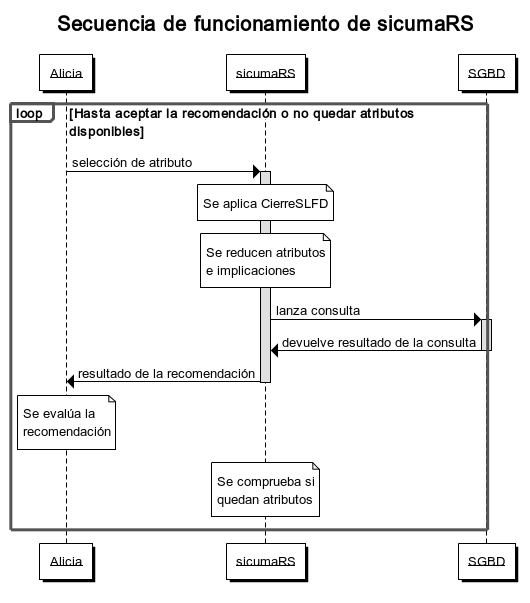
\includegraphics[height=.7\textheight,width=.8\textwidth]{diagramaSecuenciasicumaRS.png}
	\end{center}
	\caption{Diagrama de secuencia del funcionamiento de \rs.}
	\label{figura:diagramaSecuenciasicumaRS}
\end{figure}

Las Figuras \ref{figura:esquemaConversacional} y \ref{figura:diagramaSecuenciasicumaRS} nos ayudan a entender con mayor facilidad la sucesi�n de pasos que da el sistema conversacional para interactuar con el usuario y proponer recomendaciones. La primera representa el diagrama de secuencia del proceso en el cual intervienen el usuario (Alicia), el SR (en este caso \rs) y el sistema gestor de bases de datos (SGBD). Por otro lado, la Figura \ref{figura:esquemaConversacional} nos muestra un esquema conceptual aplicado a un caso determinado de la investigaci�n realizada. En concreto, ese esquema representa el funcionamiento de \rse sobre un \textit{dataset} que agrupa informaci�n sobre anomal�as hematol�gicas y fenotipos. Por tanto en el esquema podemos ver como se desarrolla un hipot�tico di�logo hasta alcanzar una lista de anomal�as aceptable. Esta figura tiene una importancia mayor a�adida ya que adem�s de servir para ilustrar el funcionamiento del SR, muestra la ganancia que obtenemos al utilizar el \cierree frente a implementaciones cl�sicas. Los resultados de aplicaci�n sobre este \textit{dataset} concreto pueden verse con mayor detalle en \cite{Benito-Picazo2017}.
 
\begin{figure}[htbp]
	\begin{center}
		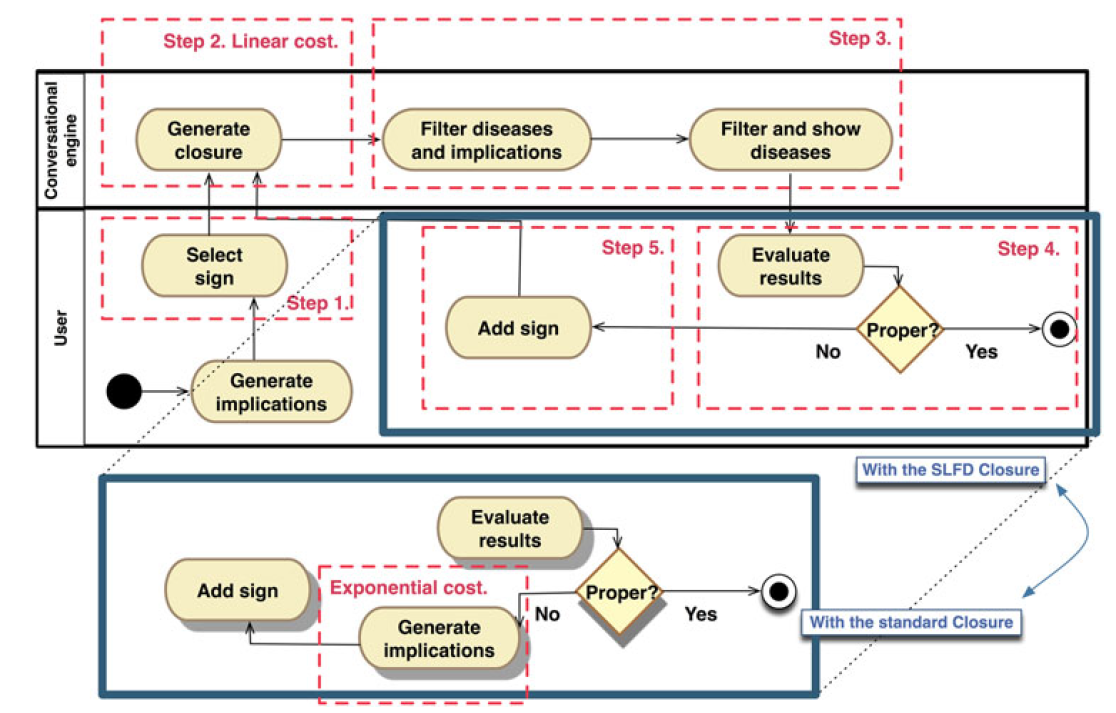
\includegraphics[height=.5\textheight,width=.95\textwidth]{esquemaConversacional.png}
	\end{center}
	\caption{Di�logo entre el usuario y \rse que muestra el funcionamiento del sistema y la ganancia obtenida por el algoritmo \cierree frente al algoritmo cl�sico del cierre. Fuente \cite{Benito-Picazo2017}.}
	\label{figura:esquemaConversacional}
\end{figure}

Finalmente, vamos a terminar este apartado mostrando un ejemplo de aplicaci�n del SR conversacional utilizando el \textit{dataset} de restaurantes que muestran los autores en \cite{LeivaERCMG13}. 

Este \textit{dataset} va a contar con 6 tipos diferentes de establecimientos que se relacionan con 11 facilidades que pueden ofrecer. La Tabla \ref{tabla:restaurants} muestra un extracto del aspecto del \textit{dataset}.

\begin{table*}[htbp]
\caption{\textit{Dataset} de restaurantes (extracto)}
\label{tabla:restaurants} 
\centering
{\scriptsize
\begin{tabular}{lccccccc}
\hline
Tipo de local & Abierto & Cerrado & Tranquilo & Animado & Pintoresco & Barato\\
\hline
Restaurante com�n & \checkmark & \checkmark & & \checkmark &  \\
%\hline
Estrella Michel�n & & \checkmark & \checkmark & &  &  \\
%\hline
Burger &  & \checkmark &  & \checkmark &  & \checkmark  \\
%\hline
Bar Tapas &  & \checkmark &  & \checkmark & \checkmark & \checkmark  \\
%\hline
Pizzer�a &  & \checkmark &  & \checkmark &  & \checkmark  \\
%\hline
Chiringuito Playa & \checkmark &  &  & \checkmark & \checkmark &  \\
\hline
\end{tabular}
}
\end{table*}

Como consecuencia, vamos a tener un conjunto de atributos \textit{U = \{Abierto, Cerrado, Tranquilo, Animado, Pintoresco, Barato, Moderado, Caro, Aire Acondicionado (AC), Vistas, Terraza\}}. Adem�s, una vez que hayamos utilizado alguna de las t�cnicas existentes para extraer las implicaciones que se verifican en la Tabla \ref{tabla:restaurants} obtenemos el siguiente conjunto de implicaciones:

%$\Gamma$ = \{$Terraza \rightarrow Animado;$ $Vistas \rightarrow Abierto, Animado, Pintoresco, Moderado, Terraza;$ $AC \rightarrow Cerrado;$ $Caro \rightarrow Cerrado, Tranquilo, AC;$ $Moderado \rightarrow Pintoresco;$ $Barato \rightarrow Cerrado, Animado;$ $Animado, Pintoresco, Terraza \rightarrow Abierto, Moderado, Vistas;$ $Animado, Pintoresco, Moderado \rightarrow Abierto, Vistas, Terraza;$ $Tranquilo \rightarrow Cerrado, AC;$ $Cerrado, Pintoresco, AC \rightarrow Tranquilo, Moderado;$ $Cerrado, Pintoresco, Moderado \rightarrow Tranquilo, AC;$ $Cerrado, Animado \rightarrow Barato;$ $Cerrado, Animado, Barato, Terraza \rightarrow AC;$ $Cerrado, Animado, Barato, AC \rightarrow Terraza;$ $Abierto \rightarrow Animado, Pintoresco, Moderado, Vistas, Terraza$\}.

\begin{itemize}
	\item $Terraza \rightarrow Animado;$
	\item $Vistas \rightarrow Abierto, Animado, Pintoresco, Moderado, Terraza;$
	\item $AC \rightarrow Cerrado;$
	\item $Caro \rightarrow Cerrado, Tranquilo, AC;$
	\item $Moderado \rightarrow Pintoresco;$
	\item $Barato \rightarrow Cerrado, Animado;$
	\item $Animado, Pintoresco, Terraza \rightarrow Abierto, Moderado, Vistas;$
	\item $Animado, Pintoresco, Moderado \rightarrow Abierto, Vistas, Terraza;$
	\item $Tranquilo \rightarrow Cerrado, AC;$
	\item $Cerrado, Pintoresco, AC \rightarrow Tranquilo, Moderado;$
	\item $Cerrado, Pintoresco, Moderado \rightarrow Tranquilo, AC;$
	\item $Cerrado, Animado \rightarrow Barato;$
	\item $Cerrado, Animado, Barato, Terraza \rightarrow AC;$
	\item $Cerrado, Animado, Barato, AC \rightarrow Terraza;$
	\item $Abierto \rightarrow Animado, Pintoresco, Moderado, Vistas, Terraza;$
\end{itemize}

En definitiva, el SR conversacional va a contar con unos datos de partida formados por: un conjunto de 6 restaurantes, 11 posibles atributos y 15 implicaciones que se verifican en los datos. Por tanto, pasemos ahora a realizar una simulaci�n de posible di�logo.

\begin{ejemplo}
\label{ejemplo:restaurantes}
Supongamos que un usuario busca una recomendaci�n sobre un restaurante para cenar. En primer lugar, busca que el lugar cuente con un atm�sfera animada. Adem�s, debido al buen clima reinante esta noche, es preferible que el establecimiento cuente con terraza. Para terminar, un precio moderado pondr�a la guinda al pastel.

De esta forma, el usuario comienza la interacci�n con el sistema introduciendo sus preferencias: \emph{Animado}, \emph{Terraza} y \emph{Moderado} de forma sucesiva y los resultados que se obtienen los podemos ver desglosados en la Tabla \ref{tabla:ejemploRestaurantes}. 

\begin{table*}[htbp]
\caption{Desglose paso a paso del di�logo entre el usuario y \rs.}
\label{tabla:ejemploRestaurantes} 
\centering
{\scriptsize
\begin{tabular}{rlllrl}
%\hline
%\multicolumn{2}{c}{Restaurants} & No. Attributes: 11 & No. Implications: 15 & No. Associations: 17 & Product T-Norm & Threshold: 0.9\\
%\hline
\hline
Iter. & Selecci�n & Cierre & Atributos & Implics. & Resultados\\
% &       &           &         & Attributes & Implications & \\
\hline
1 & Animado & \{Animado\} & \{CS, Pintoresco,& 14 & \{Burguer,\\
  &  &  & Barato, OS,& & Pizzer�a,\\
  &  &  & Tranquilo, Moderado, & & Tapas,\\
  &  &  & Caro, AC, & & Playa\}\\
  &  &  & Vistas, Terraza\} & \\
%\hline
2 & Terraza & \{Animado, Terraza\} & \{CS, Pintoresco,& 13 & \{Pizzer�a,\\
  &  &  &  Barato, OS,& & Playa\}\\
  &  &  &  Tranquilo, Moderado,& & \\
  &  &  &  Caro, AC,& & \\
  &  &  &  Vistas\} & \\ 
3 & Moderado & \{Animado, Terraza, & \{CS, Barato, & 7 & \cellcolor{gray!25}\{Playa\}\\
  &  & Moderado, OS, & Tranquilo, Caro, & \\
  &  & Pintoresco, Vistas\} & AC\} & \\
\hline
\end{tabular}
}
\end{table*}
\end{ejemplo}

De este ejemplo podemos extraer algunas conclusiones interesantes que recogemos en la lista siguiente:
\begin{itemize}
	\item Primero y m�s importante; hemos conseguido que la interacci�n con el usuario sea m�s sencilla ya que no hay necesidad de tener que tratar con todos los atributos posibles a cada paso de la conversaci�n. En cada momento, el sistema ha ido eliminando aquellos atributos que por la selecci�n de otros se encuentran impl�citamente incluidos. Gracias a ello, el di�logo entre el usuario y el sistema se hace m�s din�mico por dos razones: 
	\begin{enumerate}
		\item Se evita que los usuarios tengan que navegar entre atributos redundantes.
		\item La lista de atributos disponible depende de las elecciones previas, por tanto, los resultados pueden diferir entre un acceso al sistema y otro, evitando de esta forma obtener siempre los mismos resultados una y otra vez.
	\end{enumerate}  
	\item Gracias al algoritmo \cierre, conseguimos que en cada paso de la conversaci�n, una vez aplicado, se reduzcan tanto el n�mero de atributos disponible como el n�mero de implicaciones, lo que redunda en una reducci�n de los tiempos de respuesta del sistema.
	\item Tambi�n hemos de comentar que puede ocurrir que el usuario obtenga una recomendaci�n satisfactoria antes de que la lista de resultados tenga una longitud manejable. En estos casos, el di�logo entre el usuario y el sistema puede acabar con una lista de posibles alternativas todav�a muy extensa, pero en cualquier caso el sistema habr� guiado de forma eficiente al usuario hasta este punto. De hecho, en caso de no estar del todo satisfecho todav�a, la soluci�n pasa por continuar eligiendo atributos hasta que la lista de resultados sea m�s tratable, pero en cualquier caso, el sistema depende de la iniciativa del usuario.
\end{itemize}






\section{Medidas de evaluaci�n}
\label{seccion:medidasEvaluacion}
Como es razonable, todo sistema debe someterse a una serie de evaluaciones que confirmen su viabilidad y su utilidad. Con \rse hemos realizado este tipo de evaluaciones y para ello vamos a pasar a definir qu� medidas se han utilizado para llevar a cabo esta evaluaci�n.

Recordemos que en apartados sucesivos se analizaron muchas de las diferentes m�tricas de evaluaci�n de los SR que existen en la literatura. Sin embargo, no todas son adecuadas para todos los SR; dependiendo del SR habr� unas que sean razonables de aplicar y otras que no tengan cabida. En nuestro caso, dado que estamos tratando con un SR conversacional, puede ser evidente que la primera medida que podemos aplicar es calcular el n�mero de pasos que se producen en la conversaci�n \cite{McSherry01} como hemos estado viendo en los ejemplos anteriores. Por contra, otras m�tricas tan populares como son \textit{Precision} y \textit{Recall} \cite{Gunawardana2015} no son adecuadas de aplicar en nuestro caso porque obtendr�amos siempre valores m�ximos en ambas m�tricas y la raz�n es la siguiente:
\begin{itemize}
	\item En primer lugar, cualquier �tem de la lista de resultados, verifica los atributos seleccionados ya que la consulta que se lanza a la base de datos para obtener la lista de �tems contiene esas restricciones.
	\item Y en segundo lugar, a cada paso del di�logo, el sistema devuelve todos los �tems que verifiquen la selecci�n de atributos establecida por el usuario.
\end{itemize}
 
Sucede una situaci�n similar cuando estamos hablando de otras m�tricas muy utilizadas como son MAE o RMSE. Estas m�tricas basadas en valoraciones no tienen cabida en nuestro sistema puesto que no existen valoraciones con la que el sistema trabaje. 

Asimismo, no existe la necesidad de de considerar m�tricas referentes a la exactitud de los resultados ya que \rse no es un modelo de predicci�n, su funcionamiento est� basado en implicaciones y eso nos asegura un 100\% de exactitud en las respuestas. 

Afortunadamente, existen otras medidas que pueden reflejar los resultados de los experimentos. Las explicamos a continuaci�n:

\subsubsection*{N�mero de pasos ($N$)}
\noindent
Como su nombre indica, esta m�trica registra el n�mero de pasos que se dan en el di�logo y en consecuencia, el n�mero de atributos seleccionados por el usuario. Nos proporciona una visi�n clara de si el sistema ha necesitado mucha o poca interacci�n para satisfacer la demanda del usuario. Hay que aclarar, sin p�rdida de generalidad, que en los experimentos realizados, dependiendo del \textit{dataset} sobre el que trabajemos, se ha establecido un tama�o m�ximo de la lista de resultados como indicador de aceptaci�n por parte del usuario; por ejemplo, se establece que el usuario se considera satisfecho cuando una recomendaci�n de hoteles contenga como m�ximo 10 hoteles. 

\[ N = |\text{Atributos seleccionados}|, \quad \text{donde $|A|$ representa el cardinal de A.}\]

\subsubsection*{Velocidad de poda en cada paso i ($S_i$)}
\noindent
Esta m�trica eval�a el porcentaje de atributos que el sistema libera al usuario de tener en cuenta a lo largo de la conversaci�n y de forma acumulativa de un paso al siguiente. Con esta m�trica buscamos averiguar si los ratios de poda del algoritmo son mejores al principio de la conversaci�n o en los pasos posteriores. Es una m�trica para medir cu�n r�pido es el sistema reduciendo la sobrecarga de informaci�n.

\[ S_{i} = \frac{|\text{Atributos del cierre}|_{i} - i}{|\text{M}|}\] 
Siendo $i = 1,...,N$, y $M$ el conjunto global de atributos.


\subsubsection*{Reducci�n de atributos ($P$)}
\noindent
Esta �ltima m�trica nos informa de la reducci�n global de atributos que ha realizado el sistema al terminar el di�logo. La reducci�n de estos atributos es consistente ya que es fruto de la aplicaci�n del algoritmo del cierre a partir de las selecciones realizadas por el usuario. Formalmente:
\[ P = S_N \]

%Con la presentaci�n de las m�tricas de evaluaci�n, tenemos ya todo lo necesario para poder realizar experimentos. No obstante, puesto que los experimentos van a llevarse a cabo sobre \textit{datasets} que todav�a no han sido presentados, en el siguiente apartado vamos a detallar la naturaleza y la procedencia de cada uno de ellos como paso previo y necesario a la secci�n de experimentos propiamente dicha.




\chapter{Experimentos realizados}
\label{cap:experimentosSR}

\pagestyle{headings}

\bigdrop{0pt}{5}{cmr10}A lo largo del texto, se han mostrado ejemplos \ref{ejemplo:basico} \ref{ejemplo:restaurantes} de aplicaci�n del algoritmo \cierree y en general del SR desarrollado, no obstante, en estos momentos en los que contamos con \rse como un SR ya definido, abordamos en este cap�tulo una serie de experimentos m�s elaborados que nos permitan comprobar el funcionamiento de nuestro sistema y evaluar su rendimiento. La forma en que vamos a proceder con los experimentos la exponemos a continuaci�n.

Para cada experimento vamos a realizar un test que consiste en simular 100 di�logos siguiendo al pie de la letra el proceso detallado en \ref{seccion:funcionamiento}. No obstante, las simulaciones van a llevarse a cabo como di�logos aleatorios, es decir, cada di�logo se desarrollar� eligiendo atributos de forma aleatoria del conjunto de atributos disponible a cada paso de la conversaci�n. Esto puede verse desde diferentes perspectivas. En primera instancia, parece adecuada la estrategia aleatoria ya que as� se garantiza la honestidad de los resultados al no haber posibilidad de inducir situaciones favorables para que el sistema obtenga mejores resultados. Sin embargo, proceder de manera aleatoria tambi�n puede obscurecer las virtudes de nuestro sistema. 

Por un lado, imaginemos una situaci�n en la que las elecciones aleatorias impliquen atributos que no guardan relaci�n entre ellos en el \textit{dataset}, entonces, el di�logo terminar� r�pidamente ya que puede que haya muy pocos �tems (o incluso ninguno) que verifiquen tal selecci�n de atributos y por tanto, el proceso terminar� sin poder aplicar ninguna reducci�n de atributos. Ahora bien, supongamos un di�logo m�s realista en el que la elecci�n de atributos tenga un relaci�n m�s sensata. En este caso, durante el di�logo, el sistema ser� capaz de ir aplicando sucesivas podas para reducir la sobrecarga de informaci�n ya que existir� relaci�n entre los atributos seleccionados. Por tanto, esta forma de proceder ensalzar�a los beneficios de nuestro sistema.

En relaci�n a la evaluaci�n del sistema, las m�tricas que vamos a utilizar sobre cada simulaci�n van a a ser: n�mero de pasos de la conversaci�n, velocidad de poda de atributos en cada paso y reducci�n total de atributos; tal y como se han presentado en \ref{seccion:medidasEvaluacion}.

Finalmente, se realizan una serie de repeticiones sobre cada uno de los experimentos de manera que cada n�mero mostrado es fruto de un estudio estad�stico a partir de los resultados obtenidos en esas repeticiones que nos permite extraer los resultados m�s fiables \cite{Goh10}.

Dicho eso, el cap�tulo va a estar dividido en 4 bloques principales. Comenzaremos con un experimento sobre un \textit{dataset} muy conocido en el campo de los SR: MovieLens10M \ref{seccion:movieLensDatasets}. Es un \textit{dataset} que contiene una gran cantidad de informaci�n sobre pel�culas de la que vamos a usar s�lo los t�tulos y g�neros. En virtud de esto, trabajamos sobre una cantidad importante de elementos, pero sin contar con demasiados atributos. Continuaremos con otro \textit{dataset} que contiene un menor n�mero de elementos pero muy definidos mediante muchos atributos (Costa del Sol Hotels) y que adem�s contiene informaci�n real extra�da directamente desde la red \ref{seccion:hotelesCostaDelSol}. Para culminar esta secci�n, el �ltimo experimento utiliza un \textit{dataset} (World Wide POIs) que supera ampliamente a los anteriores en cuanto al n�mero de elementos y atributos y que al igual que el anterior, la informaci�n que presenta tambi�n es real \ref{seccion:POIsMundial}. 

Finalmente, la �ltima secci�n nos trae la presentaci�n y los resultados obtenidos sobre el \textit{dataset} \ref{seccion:sintomasDataset} utilizado en una de las publicaciones que avalan esta tesis \cite{Benito-Picazo2017}. Varias tablas y figuras acompa�ar�n cada experimento con la intenci�n de ilustrar m�s f�cilmente los resultados obtenidos. 



\section{MovieLens \textit{datasets}}
\label{seccion:movieLensDatasets}
MovieLens\footnote{http://movielens.org} es un proyecto desarrollado por el equipo de investigaci�n GroupLens\footnote{https://grouplens.org} del Departamento de Ciencias de la Computaci�n e Ingenier�a de la Universidad de Minnesota especializado en SR, comunidades online, bibliotecas digitales, ... En su direcci�n web se ayuda a la gente a elegir pel�culas que deseen ver; grosso modo es un SR de pel�culas con un tinte evidente de CF. Cuenta con cientos de miles de usuarios y de pel�culas almacenadas en una colecci�n muy rica de \textit{datasets} que han sido un referente a la hora de probar el funcionamiento de otros sistemas en diferentes entornos \cite{Harper2016}.

En nuestro caso, nos vamos a centrar en su MovieLens10M \textit{dataset}. Es un \textit{dataset} totalmente accesible de forma gratu�ta desde la p�gina web y contiene informaci�n de m�s de 10.000 pel�culas con sus respectivos g�neros, duraci�n, pa�s, valoraciones, elenco, etc.%, como muestra la Figura \ref{figura:castilloEnElCielo}.

%\begin{figure}[htbp]
%	\begin{center}
%		\includegraphics[height=.5\textheight,width=.9\textwidth]{castilloEnElCielo.png}
%	\end{center}
%	\caption{Ejemplo de los datos contenidos en la descripci�n de una pel�cula dentro del \textit{dataset} MovieLens 10M.}
%	\label{figura:castilloEnElCielo}
%\end{figure}

De toda esta informaci�n, vamos a generar un conjunto reducido para utilizarlo en nuestro \rs. Concretamente, vamos a crear una tabla para emparejar cada una de las pel�culas con todos los posibles g�neros que existen en el \textit{dataset} original. De esta forma, tendremos las pel�culas en las filas de la tabla y los g�neros como columnas; una pel�cula tendr� una marca de verificaci�n en aquellos g�neros en los que est� clasificada y nada en otro caso. La Tabla \ref{tabla:MovieLens10M} muestra un peque�o extracto del conjunto final.

\begin{table*}[htbp]
\caption{Extracto del \textit{dataset} MovieLens 10M.}
\label{tabla:MovieLens10M}
\centering
{\scriptsize
\begin{tabular}{lccccccccccccccccccccc}
\hline
T�tulo & Acci�n & Comedia & Crimen & Drama & Romance & \ldots\\
\hline
Little City (1998) &  & \checkmark &  &   &  \checkmark\\
Driver, The (1978) & \checkmark &  & \checkmark &  &   & \\
Father of the Bride (1950) &  & \checkmark &   & \\
Bio-Dome (1996) &  & \checkmark & &  &   \\
Fast Runner, The (2001) &  &  & & \checkmark &  \\
Overboard (1987) &  & \checkmark &  &  &   \checkmark  \\
Get Rich or Die Tryin' (2005) & \checkmark &  & \checkmark & \checkmark & \\
\ldots\\
\hline
\end{tabular}
}
\end{table*}

Para convertir esta informaci�n a valores de 1 � 0 para nuestro SR s�lo tenemos que cambiar los marcas de verificaci�n por 1 y el resto por 0.

Los n�meros de este \textit{dataset} adaptado seg�n se ha indicado, alcanzan los siguientes valores:
\begin{itemize}
	\item Filas (items): 10.681 pel�culas.
	\item Columnas (atributos): 19 g�neros.
	\item Implicaciones: 245
\end{itemize}

Con esta informaci�n ya estamos en disposici�n de iniciar la interacci�n entre el usuario y \rs. No obstante, antes de pasar al experimento general, veamos un ejemplo concreto de di�logo.
\begin{ejemplo}
Supongamos en este caso que el usuario est� buscando una pel�cula de acci�n, con experiencia IMAX y con algunos toques de misterio. Entonces, el usuario interact�a con el sistema introduciendo estas preferencias en la conversaci�n. El resultado lo podemos apreciar viendo cu�l ha sido di�logo que se ha producido en la Tabla \ref{tabla:ejemploMovieLens10M}.

\begin{table*}[htbp]
\caption{Resultados del di�logo entre \rse y el usuario sobre el \textit{dataset} MovieLens 10M.}
\label{tabla:ejemploMovieLens10M} 
\centering
{\scriptsize
\begin{tabular}{rllrrr}
%\hline
%\multicolumn{6 }{l}{MovieLens10M. Attributes: 19, Associations: 252, Hamacher T-Norm, Threshold: 0.5} \\
%\hline
\hline
Iter. & Selecci�n & Cierre & Atribs. & Implics. & Items\\
\hline
1 & Acci�n & \{Acci�n, Thriller, Aventura\} & 16 & 121 & 1.473\\
2 & IMAX & \{Acci�n, Thriller, Aventura, Sci-Fi, & 12 & 43 & 108\\
 &   & IMAX, Comedia, Fantas�a\} &  &  & \\
3 & Misterio & \{Acci�n, Thriller, Aventura, Sci-Fi, & 8 & 1 & 6\\
 &   & IMAX, Comedia, Fantas�a, Misterio &  &  & \\
 &   & Crimen, Romance, Cine-Negro\}\\
\hline
\end{tabular}
}
\end{table*}
\end{ejemplo}

En el ejemplo anterior, podemos darnos cuenta de que incluso cuando interactuamos con un \textit{dataset} muy grande como MovieLens10M, se hace m�s c�modo para el usuario el obtener una recomendaci�n, ya que en cada paso estamos reduciendo el espacio de b�squeda. Efectivamente, 3 pasos son suficientes para obtener la recomendaci�n entre todo el \textit{dataset}. 

En este sentido, si nos centramos en la primera iteraci�n en la que se introduce la preferencia \textit{Acci�n}, el conjunto de cierre contiene dos atributos m�s aparte del seleccionado. La siguiente iteraci�n sigue la misma l�nea y el cardinal del conjunto cierre aumenta sustancialmente. Como consecuencia, podemos liberar el usuario de tratar con esos atributos en las iteraciones sucesivas, y as� estamos reduciendo la sobrecarga de informaci�n. Adem�s, como hemos mencionado antes, al mismo tiempo, tambi�n reducimos el n�mero de implicaciones involucradas de forma significativa, lo cual acelera las consultas subsiguientes.

\vspace{0.3cm}
Una vez visto un caso concreto de di�logo con este \textit{dataset}, pasamos ahora a realizar el experimento completo tal y como se ha establecido anteriormente, es decir, simulando 100 di�logos diferentes en los cuales los atributos se eligen de forma aleatoria. La Figura \ref{figura:experimentoMovieLens10M} muestra el resultado de este experimento dividido en 3 secciones:
\begin{itemize}
	\item [a)] Representa por medio de un diagrama de sectores el porcentaje de experimentos que han necesitado un determinado n�mero de pasos para alcanzar una recomendaci�n admisible.
	\item [b)] Muestra el porcentaje total de atributos que se han reducido en el di�logo.
	\item [c)] Muestra el porcentaje de atributos que se ha reducido a cada paso de la conversaci�n, es decir, la velocidad de poda.
\end{itemize}

\begin{figure}[htbp]
	\begin{center}
		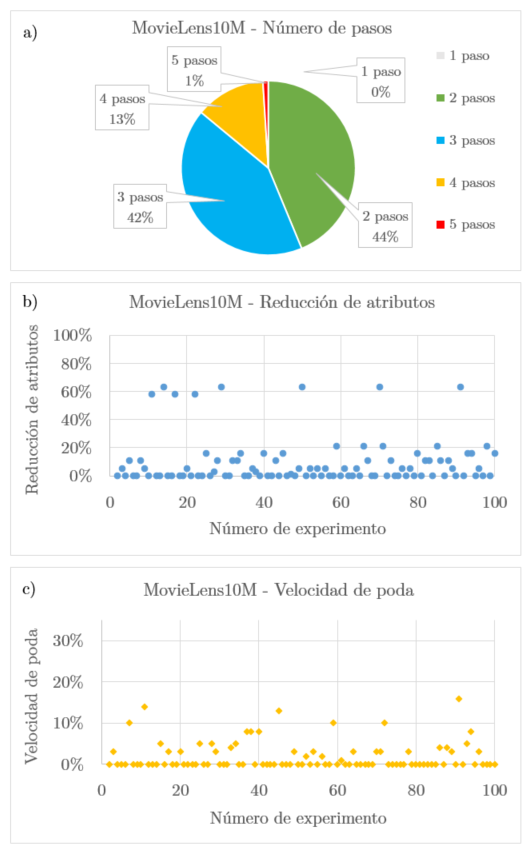
\includegraphics[height=1\textheight,width=.95\textwidth]{experimentoMovieLens10M.png}
	\end{center}
	\caption{Resultado del experimento sobre el \textit{dataset} MovieLens10M.}
	\label{figura:experimentoMovieLens10M}
\end{figure}

Al analizar la Figura \ref{figura:experimentoMovieLens10M}(a) podemos apreciar como \rse es capaz de guiar al usuario hasta una recomendaci�n aceptable en 2 � 3 pasos en la mayor�a de los casos. Si tenemos en cuenta el tama�o de este \textit{dataset}, estos resultados son altamente prometedores.

Respecto a la reducci�n de atributos global, la Figura \ref{figura:experimentoMovieLens10M}(b) muestra que el sistema ha liberado al usuario de tener que interactuar con el 5-20\% de los atributos. Incluso tenemos algunas pruebas en las que la reducci�n ha llegado a alcanzar el 60\% de los atributos.

La velocidad de poda acompa�a el resultado anterior movi�ndose en un rango de entre el 2-10\% como muestra la Figura \ref{figura:experimentoMovieLens10M}(c).

A la luz de estos resultados, podemos concluir que \rse se comporta de forma notable a la hora de aliviar la sobrecarga de informaci�n en la interacci�n con el usuario.

\begin{remark}
Aparte de los \textit{dataset} que podemos encontrar disponibles en la web, a la hora de realizar experimentos nos vimos en la necesidad de poder crear nuestros propios \textit{datasets}, igualmente utilizando informaci�n real, pero ahorrando los pasos de an�lisis y preparaci�n de la informaci�n al formato de \rs. 

A ra�z de ello, se investig� el \textit{web-scrapping} como una de las t�cnicas disponibles para extraer informaci�n de la red \cite{Bonifacio2015,Johansson2015}. El aprendizaje de esta t�cnica nos abri� la puerta a crear \textit{datasets} con los que poder trabajar. Como ejemplo de algunos de ellos, tenemos el \textit{dataset} de Hoteles Costa del Sol cuyo experimento pasaremos a analizar, y el de puntos de inter�s tur�stico (POIs Mundial) que veremos en la secci�n \ref{seccion:POIsMundial}.
\end{remark}


\section{Hoteles Costa del Sol \textit{dataset}}
\label{seccion:hotelesCostaDelSol}
Este experimento tiene un gran inter�s para el usuario ya que la elecci�n de un hotel, ya sea por vacaciones, trabajo o cualquier otro motivo, suele ser una decisi�n con un alto margen de maniobra en primera instancia. Por lo tanto, contar con un sistema que acelere la b�squeda de nuestras necesidades puede ser muy �til para ahorrar tiempo y esfuerzo. Para ello, presentamos un \textit{dataset} que contiene m�s de 300 hoteles (extra�dos del proyecto Costa del Sol Occidental\footnote{http://www.costadelsoloccidental.org}) cada uno de los cuales con 37 atributos diferentes. Aunque el \textit{dataset} es muy disperso, la tabla final obtenida es digna de tener en consideraci�n ya que est� formada por informaci�n real que se utiliza actualmente por muchos turistas que visitan el sur de Espa�a. 

Al igual que en el experimento anterior, vamos a generar una tabla que contiene los hoteles en las filas y las caracter�sticas o servicios en las columnas tal y como se muestra en la Tabla \ref{tabla:hotelesDataset}.

\begin{table*}[tb]
\caption{Hoteles Costa del Sol \textit{dataset} (extracto)}
\label{tabla:hotelesDataset} 
\centering
{\scriptsize
\begin{tabular}{lcccccccccccccccccccc}
\hline
Nombre Hotel & AC & Bar & Gym & Internet & Masajes & Parking & \ldots\\
\hline
Fuerte Estepona Suites & \checkmark & \checkmark & \checkmark & \checkmark & \checkmark & \checkmark\\
Hotel Buenavista &  & \checkmark &  &  &  & \checkmark \\
Hotel Paraiso & \checkmark & \checkmark &  &  &  & \checkmark \\
Apts Marriot Playa &  &  &  & \checkmark &  &  \\
Hotel Piedra Paloma &  & \checkmark &  &  &  & \checkmark \\
Hostal Hospederia V Cent & \checkmark & \checkmark &  & \checkmark &  & \checkmark \\
\ldots\\
\hline
\end{tabular}
}
\end{table*}

Si bien es cierto que este \textit{dataset} no contiene tantos elementos como el de MovieLens10M \ref{seccion:movieLensDatasets}, s� que lo supera en n�mero de atributos para cada �tem, y a�n m�s importante, en el cardinal del conjunto de implicaciones. Los n�meros finales son:
\begin{itemize}
	\item Filas (items): 361 hoteles.
	\item Columnas (atributos): 37 servicios.
	\item Implicaciones: 1.507
\end{itemize}

Al igual que en el experimento anterior, antes de entrar en el experimento general, veamos un caso concreto. 

\begin{ejemplo}
Supongamos que una pareja joven quiere pasar un fin de semana descansando en un hotel y est�n visitando sitios web en un tel�fono m�vil. Los requisitos que buscan por parte del hotel son \textit{Spa} y servicio de \textit{Belleza}. Al introducir estos par�metros en el sistema, se produce un resultado con 16 hoteles. Un resultado as� puede ser inc�modo para la pantalla de un tel�fono m�vil com�n. Sin embargo, consideran incluir una sesi�n de \textit{Masaje} tambi�n, por tanto, a�aden la nueva preferencia y obtienen una lista de recomendaci�n con 7 hoteles, eso ya es aceptable. El proceso se representa en la Tabla \ref{tabla:hotelesConversacion}.

\begin{table*}[htbp]
\caption{Resultados del di�logo entre \rse y el usuario sobre el \textit{dataset} Hoteles Costa del Sol}
\label{tabla:hotelesConversacion} 
\centering
{\scriptsize
\begin{tabular}{rllrrr}
%\hline
%\multicolumn{6 }{l}{Costa del Sol Hotels. Attributes: 37, Associations: 3.872, Nilpotent T-Norm, Threshold: 0.1}\\
%\hline
\hline
Iter. & Selecci�n & Cierre & Atribs. & Implics. & Items\\
\hline
1 & Spa & \{Spa, Bar, Restaurante, Cafeter�a, & 29 & 799 & 96\\
  &     & Piscina, Jardines, Parking, AC\} & & & \\
2 & Belleza & \{Spa, Bar, Restaurante, Cafeter�a, & 25 & 559 & 16\\
  &     & Piscina, Jardines, Parking, AC\} & & & \\
  &     & Belleza, Reuniones, Deporte, Animaci�n\} & & & \\
3 & Masaje & \{Spa, Bar, Restaurante, Cafeter�a, & 21 & 126 & 7\\
  &     & Piscina, Jardines, Parking, AC, & & & \\
  &     & Belleza, Reuniones, Deporte, Animaci�n, & & & \\
  &     & Masaje, M�dico, Lavander�a, Internet\} & & & \\
\hline
\end{tabular}
}
\end{table*}
\end{ejemplo}

En este experimento se aprecia claramente c�mo el mecanismo de poda hace que la interacci�n sea m�s r�pida, m�s c�moda y din�mica, ya que podr�a ser una ardua tarea tratar de elegir por un hotel entre cientos de posibilidades con m�s de 30 servicios posibles cada una. Por el contrario, 3 pasos son suficientes para guiar a la pareja
a sus mejores opciones. Estos resultados superan con creces los estudios previos \cite{TrabelsiWBR11} donde, incluso contando con un \textit{dataset} hotelero m�s peque�o, el n�mero de pasos necesarios es mayor.


Con la intenci�n de preservar la completitud con el experimento anterior, la Figura \ref{figura:experimentoHotelesQualifica} muestra el resultado para el experimento completo.

\begin{figure}[htbp]
	\begin{center}
		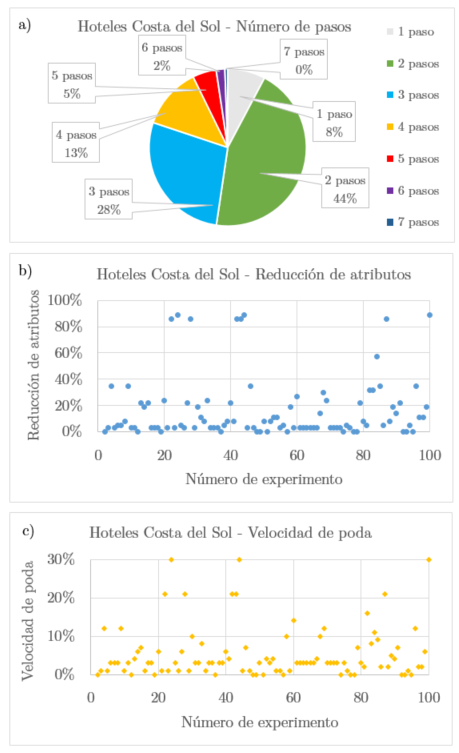
\includegraphics[height=1\textheight,width=.95\textwidth]{experimentoHotelesQualifica.png}
	\end{center}
	\caption{Resultado del experimento sobre el \textit{dataset} Hoteles Costa del Sol.}
	\label{figura:experimentoHotelesQualifica}
\end{figure}

Respecto a este experimento, podemos ver que los resultados son ligeramente diferentes a los alcanzados sobre MovieLens10M \ref{figura:experimentoMovieLens10M}. El primer punto notable del experimento es que esta vez hay casos en que la duraci�n de la conversaci�n ha aumentado y esto se debe a que el n�mero de atributos posibles es mucho mayor ahora. A�n as�, en la mayor�a de los casos son necesarios s�lo 2-3 pasos una vez m�s para conseguir una recomendaci�n admisible.

La reducci�n de atributos es mayor en este caso con respecto a MovieLens10M, alcanzando tasas de poda entre 10-40\% en la mayor�a de los casos, y de entorno al 85\% en algunos otros. 

Del mismo modo, la velocidad de poda tambi�n es mayor como podemos apreciar en la Figura \ref{figura:experimentoHotelesQualifica}(c); en definitiva, consiguiendo valores que reflejan la utilidad del mecanismo de conversacional.



\section{POIs Mundial \textit{dataset}}
\label{seccion:POIsMundial}
Finalmente, con la intenci�n de crear un \textit{datasete} m�s amplio que los anteriores tanto en el n�mero de �tems como en el n�mero de atributos, llegamos al �ltimo \textit{dataset} generado, al cual hemos denominado POIs Mundial \textit{dataset}. Manteniendo la idea de realizar pruebas m�s fidedignas, la informaci�n del \textit{dataset} es informaci�n real, extra�da del portal web Tripadvisor\footnote{https://www.tripadvisor.es} con las t�cnicas mencionadas anteriormente. Este \textit{dataset} va a contener informaci�n de multitud de puntos de inter�s (en ingl�s \textit{Points Of Interest}) tur�stico de todo el mundo (Torre Eiffel, Estatua de la Libertad, Big Ben, Plaza Roja, Coliseo, etc.). En esta clasificaci�n entran monumentos, parques, museos, iglesias, galer�as de arte, teatros, complejos deportivos, ..., as� hasta un total de m�s de 100 categor�as diferentes. En la Figura \ref{figura:poisRoma} mostramos un ejemplo de algunos de los puntos de inter�s que podemos encontrar en Roma seg�n la web y las categor�as a las que pertenecen.

\begin{figure}[htbp]
	\begin{center}
		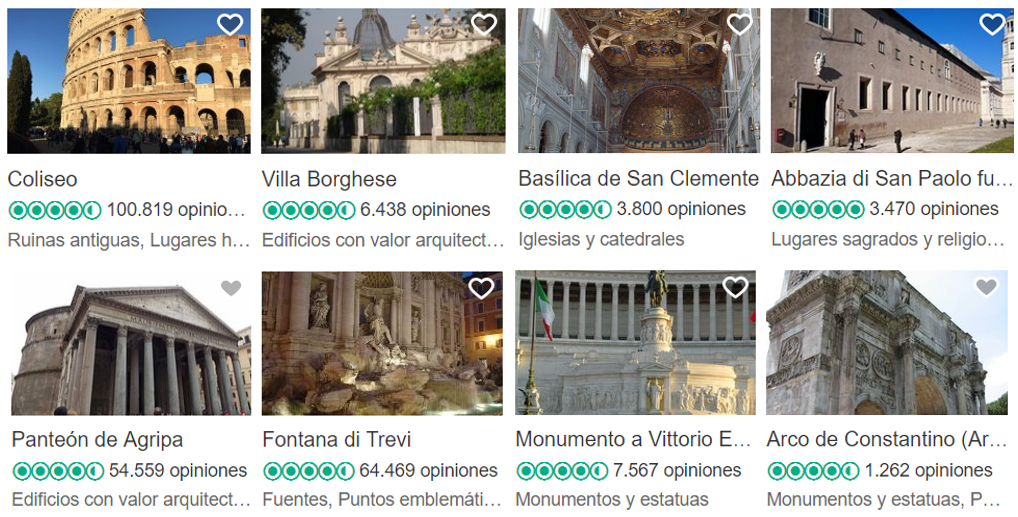
\includegraphics[height=.4\textheight,width=1\textwidth]{poisRoma.png}
	\end{center}
	\caption{Ejemplo de puntos de inter�s de la ciudad de Roma que muestra el portal Tripadvisor. En la parte inferior de cada uno podemos ver a qu� grupo pertenece (Iglesias, Monumentos, Estatuas, Fuentes, ...).}
	\label{figura:poisRoma}
\end{figure}

La generaci�n de este \textit{dataset} arroj� una serie de resultados muy satisfactorios. El primero fue constatar la capacidad adquirida para la generaci�n de \textit{datasets} de gran envergadura y con informaci�n real. De hecho POIs Mundial con un total de 17.400 puntos de inter�s (�tems), cantidad que sobrepasa notablemente a las 10.000 pel�culas almacenadas en el hist�rico \textit{dataset} de MovieLens10 analizado en \ref{seccion:movieLensDatasets}. Adem�s, cada elemento puede pertenecer a m�s de 100 categor�as diferentes (en concreto 115 categor�as diferentes), lo cual genera una tabla con un total de m�s de 2 millones de celdas. A�n as�, el n�mero de implicaciones generado no es excesivo debido a que el conjunto es altamente disperso. 

En resumen, los n�meros para este �ltimo \textit{dataset} son:
\begin{itemize}
	\item Filas (items): 17.400
	\item Columnas (atributos): 115
	\item Implicaciones: 675
\end{itemize}

Pasamos ahora comprobar el resultado obtenido tras lanzar el test sobre el mayor de los \textit{datasets} generados en esta investigaci�n.

Recordemos ahora que estamos tratando con un \textit{dataset} que contiene m�s de 17.000 puntos de inter�s que pueden verificar m�s de 100 atributos diferentes. Si bien los n�meros de este \textit{dataset} son mayores que los de el \textit{dataset} MovieLens10M, vemos que los resultados obtenidos, \textit{a priori} parecen a�n m�s espectaculares (2 � 3 pasos en la conversaci�n). Sin embargo, en este caso tenemos que hacer unas aclaraciones.

Al principio de este apartado indic�bamos que los tests se llevar�an a cabo simulando di�logos donde los atributos se seleccionar�an de forma aleatoria y analizamos los pros y contras de esta decisi�n. Bien, pues experimento pone en evidencia tales circunstancias. Por un lado, vemos como la mayor�a de los test finalizan en 2 � 3 pasos de conversaci�n (ver Figura \ref{figura:experimentoPOIsMundial}(a)). Esto puede considerarse un gran �xito del sistema al necesitar un di�logo tan corto a la hora de hacer una recomendaci�n entre tant�simos elementos, y de hecho en muchos de los tests la situaci�n se refleja fielmente. 

Sin embargo, algunos otros experimentos que tambi�n han terminado tan r�pido, se debe a que la selecci�n de atributos no ha sido coherente. Por ejemplo, supongamos que entre todos los atributos se ha seleccionado que el punto de inter�s sea del tipo \textit{Museo Hist�rico} y \textit{Playas}, entonces a la hora de buscar elementos del \textit{dataset} que verifiquen simult�neamente atributos tan dispares, el resultado contendr� muy pocos elementos y por tanto en pocos pasos habremos finalizado el di�logo. En definitiva, esto sucede debido a dos razones fundamentales: 
\begin{enumerate}
	\item La selecci�n aleatoria de atributos.
	\item Y muy importante, el \textit{dataset} es altamente disperso, ya que de entre los m�s de 100 atributos posibles, un punto de inter�s llega a verificar simult�neamente a la sumo 7 de ellos.
\end{enumerate}

Por otro lado, en la Figura \ref{figura:experimentoPOIsMundial}(b) y (c) podemos apreciar que en este caso la reducci�n de atributos y la velocidad de poda alcanzan niveles a�n m�s notables que en el caso de MovieLens10M, y es que aunque los valores sean similares (reducci�n entre el 5-25\% y velocidad de poda entre el 2-10\%), hay que tener en cuenta que debido al tama�o de este \textit{dataset}, esos porcentajes implican un n�mero de elementos eliminados muy superior.

En resumen, podemos constatar que incluso con \textit{datasets} tan ricos en contenido, \rse es capaz de entablar un di�logo con el usuario brind�ndole unas reducciones de informaci�n muy importantes, aliviando de esta forma de manera notable la sobrecarga de informaci�n.

\begin{figure}[htbp]
	\begin{center}
		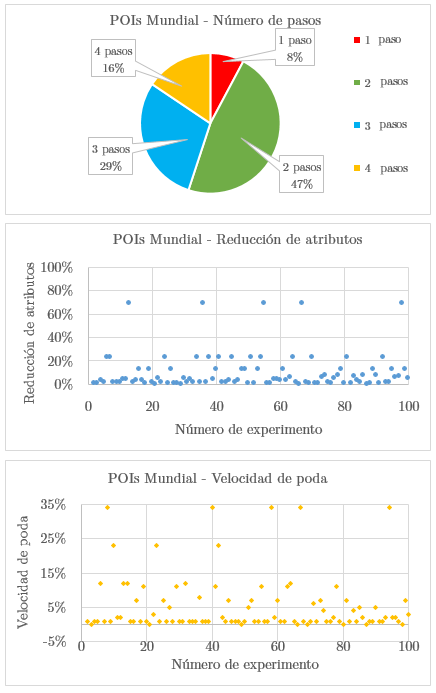
\includegraphics[height=1\textheight,width=.9\textwidth]{experimentoPOIsMundial.png}
	\end{center}
	\caption{Resultado del experimento sobre el \textit{dataset} POIs Mundial.}
	\label{figura:experimentoPOIsMundial}
\end{figure} 



%\section{Otros experimentos}
%\label{seccion:otrosExperimentos}
%Hasta ahora y como mencionamos al principio de este cap�tulo, hemos analizado el resultado de las pruebas para 3 tipos diferentes de \textit{dataset} en cuanto a contenido y caracter�sticas relacionadas con el funcionamiento de \rs. Estos resultados han demostrado claramente la operatividad de \rse y el progreso alcanzado en cuanto al tratamiento del problema de la dimensionalidad en las recomendaciones.

%No obstante, durante la realizaci�n de esta tesis se han realizado otros experimentos similares que, si bien no vamos a analizar al mismo nivel de detalle por ser parecidos a los ya expuestos, les dedicaremos una breve rese�a.

\section{Enfermedades y S�ntomas \textit{dataset}}
\label{seccion:sintomasDataset}
Otro de los \textit{datasets} generados es el que hemos denominado por cuenta propia \textit{Diseases \& Symptoms dataset}. Este \textit{dataset} tiene una importancia mayor ya que ha sido el utilizado en una de las publicaciones que avalan esta Tesis Doctoral \cite{Benito-Picazo2017}. A continuaci�n, pasamos a describir la fuente de los datos y la estructura del \textit{dataset} generado.

La fuente original de la cual se ha extra�do la informaci�n es el Phenotype Ontology Consortium\footnote{http://www.human-phenotype-ontology.org} (HPO). Como podemos leer en su p�gina web: ``HPO \footnote{HumanPhenotypeOntology} pretende proveer un lenguaje estandarizado de las fenotipos encontrados por anomal�as en enfermedades humanas. Cada t�rmino en HPO describe una anomal�a fenot�pica. HPO est� en desarrollo utilizando literatura m�dica, Orphanet\footnote{http://www.orpha.net/consor/cgi-bin/index.php}, DECIPHER\footnote{https://decipher.sanger.ac.uk}, y Online Mendelian Inheritance in Man (OMIM)\footnote{http://www.omim.org}.''.  A partir de toda esta informaci�n pudimos generar un \textit{dataset} sobre el que desempe�ar nuestros experimentos. 

Debido a que la cantidad de informaci�n en el HPO es enorme, en esta primera aproximaci�n s�lo vamos a utilizar un extracto de toda la informaci�n disponible. Haciendo uso de OMIM para diferenciar entre diferentes tipos de fenotipos que aparecen en el HPO, hemos generado una tabla que empareja anomal�as hematol�gicas y fenotipos, consiguiendo un conjunto de datos considerable. Podemos ver un extracto de la informaci�n generada en la Tabla \ref{table:diseases}.

\begin{table*}[htbp]
\caption{Diseases \& Symptoms dataset (extract)}
\label{table:diseases} \centering
{\scriptsize
\begin{tabular}{lccccccc}
\hline
Disease ID & HPO\_1249 & HPO\_1250 & HPO\_1251 & HPO\_1252 & HPO\_1254 & \ldots\\
\hline
274000 &  & \checkmark &  &   & \\
%275350 & X &  & X &  & X & \\
275630 & \checkmark &  & \checkmark & & \\
277380 &  &  &  & \checkmark & \checkmark \\
%277400 & X & X & & X & X & \\
%300653 & X & X & X &  &  & \\
300884 &  & \checkmark &  & \checkmark &  \\
300322 & \checkmark &  &  & \checkmark &  \\
\ldots\\
\hline
\end{tabular}
}
\end{table*}

En caso de que queramos obtener informaci�n detallada de cada anomal�a que se muestra, encomendamos al lector a visitar la web de OMIM y utilizar su motor de b�squeda con el identificador mostrado en la columna \textit{Disease ID}. Como ejemplo, la anomal�a \textit{Disease ID 275630} corresponde con el s�ndrome \textit{Chanarin-Dorfman}.

En definitiva, vamos a trabajar sobre un \textit{dataset} con 446 enfermedades, 100 fenotipos diferentes y todas las implicaciones que se verifican. Desgraciadamente, no podemos mostrarlas todas en el documento pues el conjunto alcanza un n�mero superior a 6.000 implicaciones. 

Este experimento adem�s de su relevancia en cuanto a figurar en una de las publicaciones que avalan esta tesis \cite{Benito-Picazo2017}, tiene una importancia a�adida debido al alto n�mero de implicaciones que contiene. Recordemos que en un \textit{dataset} de referencia en el campo como lo es MovieLens10M \ref{seccion:movieLensDatasets} el n�mero de implicaciones que obten�amos era 245, mientras que ahora \rse trabajar� y con resultados satisfactorios, con este \textit{dataset} en el que el cardinal del conjunto de implicaciones es superior a 6.000 implicaciones.

A continuaci�n recopilamos los n�meros de este \textit{dataset}:

\begin{itemize}
	\item Filas (items): 446 anomal�as.
	\item Columnas (atributos): 100 fenotipos.
	\item Implicaciones: 6.468
\end{itemize}

En este punto tenemos que hacer un inciso importante y que es de aplicaci�n para todos los \textit{datasets} y pruebas que se han realizado.

\begin{remark}
Si nos centramos en el Enfermedades y S�ntomas \textit{dataset} y calculamos la llamada base Duquenne-Guigues \cite{Guigues1986} de implicaciones que se verifican en el contexto, el n�mero de implicaciones asciende hasta las 8.811 implicaciones. Entonces, �por qu� hablamos de que el sistema va a tratar unas 6.000 implicaciones con este \textit{dataset}? Bien, pues la principal caracter�stica de la base Duquenne-Guigues de implicaciones es que esta base tiene el menor n�mero de implicaciones posibles entre todas las posibles bases de implicaciones que se verifican en el contexto. Sin embargo, existir�n algunas implicaciones para las que no haya ning�n objeto que las verifique, y esas implicaciones significan que el conjunto de objetos que pueden cumplir con la premisa de la regla, no existen en el contexto. Adem�s, esas implicaciones incluyen todos los atributos del contexto. Por tanto, el sentido de esas implicaciones es simplemente te�rico y no presenta ning�n valor cuando estamos tratando con aplicaciones reales; es por ello por lo que obviamos tales implicaciones.
\end{remark}

En este caso, los resultados del experimento y sus conclusiones pueden consultarse en \cite{Benito-Picazo2017}.

% =====================================================================
% =====================================================================
% =====================================================================



\clearemptydoublepage


\pagestyle{empty}
\chapter{Conclusiones y Trabajos Futuros}
\label{cap:conclusiones}
%\addcontentsline{toc}{chapter}{\protect{Introduction}}

%\markboth{Introduction}{Introduction}

\pagestyle{headings}

\bigdrop{0pt}{5}{cmr10}Fundamentalmente, se puede decir que esta Tesis ha englobado dos vertientes principales dada su naturaleza dual. Por un lado, se ha realizado un profundo estudio de los m�todos basados en la l�gica para el tratamiento eficiente de la informaci�n utilizando los conjuntos de implicaciones que se verifican en un determinado dataset. Y por otro lado, de forma m�s extensa, se han realizado las tareas de investigaci�n e implementaci�n necesarias para poder llevar estos m�todos te�ricos a la pr�ctica. Hemos trabajado sobre tres campos diferentes: claves minimales, generadores minimales y sistemas de recomendaci�n. Para cada uno de ellos se han realizado multitud de experimentos que demuestran la utilidad y la validez del trabajo realizado. Asimismo, se hace un especial hincapi� en la parte aplicada del estudio con la intenci�n de facilitar la transferencia de conocimiento a entornos diferentes del �mbito acad�mico, como el mercado empresarial.

En esta tesis hemos podido apreciar el hecho de que contar con una s�lida teor�a basada en la l�gica y las matem�ticas nos concede la base para la creaci�n de m�todos automatizados con los que poder afrontar el desarrollo de aplicaciones de ingenier�a. Como hemos podido comprobar, existe una gran cantidad de informaci�n impl�cita en los datos que solemos manejar. El descubrimiento de toda esta informaci�n y su gesti�n inteligente es sin duda un claro tema de investigaci�n con fuerte actividad y repercusi�n en la actualidad. Esta ha sido nuestra intenci�n a la hora de trabajar con FCA, los conjuntos de implicaciones y los operadores de cierre. Pasar de la teor�a a la pr�ctica y viceversa ha sido uno de los principales desaf�os tanto de esta tesis como lo es para el propio FCA si se pretende que se convierta en una herramienta fruct�fera para la representaci�n, gesti�n y an�lisis del conocimiento en situaciones reales.

Antes de entrar plenamente en el apartado de conclusiones, queremos indicar la manera de certificar la validez de los resultados obtenidos a lo largo de la tesis. Como hemos podido advertir en los cap�tulos anteriores, nuestra labor se centra en actuar sobre conjuntos de implicaciones. En ese sentido, para los experimentos realizados hemos contado con unos ficheros de entrada que conten�an la informaci�n necesaria, y sobre ellos hemos obtenido unos resultados. Ahora bien, la forma de verificar que esos resultados son correctos es la siguiente. En primer lugar y con respecto a los resultados de claves y generadores minimales, se han realizado y corregido numerosos ejercicios en papel intentando buscar casos l�mites donde la implementaci�n pudiera no ser precisa y se ha comprobado que los resultados obtenidos en papel coincid�an exactamente con los calculados por las implementaciones en la m�quina. Adem�s, dado que para muchos de los ejemplos probados en los que se llegaban a calcular millones de nodos de un �rbol no era posible comprobar si cada uno de esos c�lculos era correcto, para el caso concreto de los experimentos relacionados con claves minimales, la validez de los experimentos viene dada al haber cotejado los resultados con aquellos obtenidos sobre un amplio abanico de ficheros utilizados en trabajos anteriores \cite{Benito-Picazo2013PFC,Benito-Picazo2014TFM} donde su validez qued� demostrada. B�sicamente, la validez de los ejercicios m�s grandes se ha extrapolado de los resultados correctos obtenidos para los ejercicios m�s peque�os. Asimismo, los resultados se corroboran igualmente al alcanzar las mismas soluciones para diferentes m�todos cuando cada uno de ellos hace un tratamiento de la informaci�n diferente con respecto al otro. En relaci�n a los experimentos con SR conversacionales, dado que los experimentos no alcanzan n�meros tan altos, la validez puede demostrarse de forma m�s asequible siguiendo un desarrollo expl�cito en papel.

Y el otro punto que queremos remarcar es el siguiente. A lo largo de todo el proyecto siempre hemos hablado de trabajar sobre sistemas de implicaciones. No obstante, queda fuera del �mbito de esta tesis el procedimiento mediante el cual se obtiene esos elementos para un sistema de datos. Para ello, encomendamos al avezado lector a visitar \cite{HuhtalaKPT99,YaoHB2002,Yevtushenko2006}. En nuestro caso, nuestro cometido comienza con el tratamiento de la informaci�n una vez de ha extra�do el conjunto de implicaciones de un sistema concreto.

Aclarados estos puntos, nos encontramos ahora en el �ltimo cap�tulo de la Tesis, en el cual vamos a recopilar la conclusiones m�s importantes que hemos alcanzado como resultado del trabajo de investigaci�n realizado. Seguidamente, cerrar�n el cap�tulo una serie de tareas con las que continuar a partir de este punto y que se introducen como trabajos futuros.


\section*{Conclusiones}
\noindent
Como hemos mostrado anteriormente, conocer las claves es fundamental en cualquier modelo de datos. En este sentido, hemos presentado una serie de m�todos que nos permiten averiguar el conjunto de claves a partir del conjunto de implicaciones y haciendo uso de m�todos de razonamiento automatizado, en concreto, la \slfd. Se ha investigado, pasando desde la teor�a a la pr�ctica, los diferentes m�todos implementados haciendo uso del paradigma de Tableaux y se ha comprobado como, hasta donde sabemos, los resultados obtenidos superan las aproximaciones anteriores.

Por otro lado, enumerar todos los conjuntos cerrados y sus generadores minimales es un problema muy complejo pero esencial en varias �reas de conocimiento y una oportunidad para mostrar los beneficios de FCA cuando trabajamos para aplicaciones reales. Para abordar esta tarea, se han presentado dos m�todos de poda para mejorar el rendimiento de la enumeraci�n de los generadores minimales. Para ello se ha hecho un uso intensivo de la \slfde sobre conjuntos de implicaciones. Finalmente, se han creado, analizado y probado enfoques diferentes (MinGen, MinGenPr, GenMinGen), mostrando claramente las mejoras alcanzadas por cada uno.

En ambas situaciones, es decir, tanto para claves minimales como para generadores minimales, se han desarrollado los c�digos necesarios para poder actuar sobre grandes cantidades de informaci�n. No obstante, para resolver problemas reales donde la cantidad de informaci�n de entrada sea considerable, es incuestionable la necesidad de unos recursos enormes tales como los que ha proporcionado el Centro de Supercomputaci�n y Bioinnovaci�n de la Universidad de M�laga; sin ellos habr�a sido inviable haber podido realizar gran parte de las pruebas. De acuerdo con esto, es absolutamente necesario que las implementaciones tengan en cuenta el correcto uso de recursos de memoria. Incluso para problemas peque�os, la cantidad de memoria que se puede necesitar puede dispararse escandalosamente.

Asimismo, el parecido y la cualidad de independencia que tiene cada nodo del �rbol tanto para los m�todos de claves minimales como para los de generadores minimales, ponen de manifiesto que la utilizaci�n de estrategias paralelas sea la mejor opci�n para abordar estos problemas. No obstante, el primer punto que queremos aclarar es que el concepto de paralelismo que hemos utilizado se refiere a un paralelismo de tipo \textit{hardware}. Con esto nos referimos a que los beneficios que obtenemos del paralelismo se deben a la utilizaci�n de un conjunto de procesadores que se encargan de ir resolviendo cada uno de los subproblemas de forma simult�nea. Por lo tanto, no estamos ante un caso de desarrollo de c�digo paralelo desde una visi�n m�s purista, sino que es m�s acertado considerarlo como una aplicaci�n basada en una estrategia \textit{MapReduce}\cite{Dean2004}.

Para la mayor�a de los casos, en relaci�n a claves y generadores minimales, existe un serio inconveniente. En primera instancia es pr�cticamente imposible, por el momento, prever cu�l va a ser la magnitud que va a alcanzar la resoluci�n del problema a la vista de la informaci�n de entrada. Esto nos va a obligar a realizar una serie de experimentos previos de forma que podamos aproximar las necesidades que va a tener un determinado experimento. 

Para cada una de las implementaciones realizadas, exist�a la necesidad de establecer criterios que nos permitieran evaluar el rendimiento de las pruebas de forma que pudi�ramos comparar unos m�todos con otros. En el caso de los experimentos relacionados con claves y generadores minimales, cuando nos planteamos la idea de la comparaci�n de resultados, lo primero que se nos ocurri� fue la medici�n de los tiempos que necesitaba cada uno de los m�todos para obtener los resultados. No obstante, advertimos como este par�metro est� �ntimamente ligado a la arquitectura que estemos utilizando para ejecutar el experimento, lo cual hace que el resultado dependa en gran medida de los recursos que se est�n utilizando y no tanto de la calidad o eficiencia del propio algoritmo. En consecuencia, se oscurec�a la utilidad te�rica de los resultados obtenidos. Por tanto, se decidi� contabilizar magnitud del �rbol y la cantidad de resultados redundantes que se obtienen. De esta forma, si alguien hiciera otro m�todo con un c�digo en cualquier otro lenguaje o utilizase recursos \textit{hardware} diferentes que desembocaran en una mejora del tiempo, siempre podr�amos atenernos al tama�o del �rbol pudiendo defender si realmente es una mejora en el m�todo o en la ejecuci�n debido a la arquitectura.

En cuanto a los SR conversacionales, tambi�n son varias las conclusiones a las que hemos llegado. La m�s importante es que, efectivamente, el tratamiento que realizamos de la informaci�n por medio de implicaciones y la \slfde puede aplicarse con �xito en este campo de conocimiento. Esto ya quedaba patente, como hemos mencionado con anterioridad, por la existencia de multitud de trabajos en la literatura de SR que utilizan conceptos de FCA; nuestro trabajo viene a reforzar este hecho.

Concretamente, presentamos una novedosa aplicaci�n del algoritmo de cierre \cierree para afrontar el problema de la sobrecarga de la informaci�n que a menudo presentan los SR. Nuestra soluci�n propone un proceso conversacional de selecci�n de atributos por parte del usuario. Este trabajo combina caracter�sticas de sistemas basados en conteido con sistemas badados en conocimiento mediante una gesti�n inteligente de las implicaciones a trav�s del cierre \cierre. Nuestro sistema constituye un marco que puede integrarse en diversos datasets y los resultados siguen siendo admisibles. Esto es, ciertamente, una gran contribuci�n de este trabajo, pues ofrece la posibilidad de aplicarse a aplicaciones en diferentes �reas.

Otra conclusi�n importante es que existen numerosas t�cnicas de recomendaci�n. De esta forma, una tarea fundamental en el desarrollo o en el an�lisis de un SR ser� identificar qu� t�cnica es la m�s adecuada para su funcionamiento seg�n el contexto de uso esperado. Del mismo modo, es excepcionalmente dif�cil abarcar todos los aspectos que involucran a un SR para evitar los diferentes problemas que pueden aparecer, por tanto, hay que tener presente con qu� expectativas queremos que act�e. Adem�s, hay que tener en cuenta que son muy pocos los SR que basan su funcionamiento en una �nica t�cnica de recomendaci�n; lo habitual es que sean sistemas h�bridos con la intenci�n de poder beneficiarse de las ventajas que ofrecen unas estrategias de recomendaci�n y otras. Nuestro caso en un claro ejemplo; el tipo de SR desarrollado mezcla las estrategias de recomendaci�n basada en contenido, basada en conocimiento y conversacional.

Por otro lado, existen numerosas opciones a la hora de evaluar el funcionamiento de un SR. Esta es una conclusi�n razonable en tanto en cuanto el n�mero de t�cnicas diferentes con las que trabajan los SR es igualmente alto. Es fundamental decidir qu� m�tricas son oportunas de aplicar dependiendo del tipo de SR que queramos evaluar, pues evidentemente habr� casos en los que una m�trica no tenga cabida para un tipo de SR determinado. Asimismo, es recomendable no pretender obtener valores �ptimos en la mayor�a de las m�tricas. Hay que ser realista y darse cuenta de que es extremadamente dif�cil cumplir plenamente con unas y otras simult�neamente. La clave est� en decidir cu�l es el cometido principal de nuestro sistema, aplicarle las m�tricas de evaluaci�n apropiadas y sacar las conclusiones pertinentes dentro de ese marco de actuaci�n.

Finalmente, queremos remarcar que el sistema desarrollado es capaz de ir m�s all� del �mbito acad�mico o de investigaci�n. Las pruebas realizadas sobre \textit{datasets} reales demuestran la viabilidad y la utilidad que el sistema puede aportar en entornos empresariales. De esta forma, apostamos de nuevo por una eficaz transmisi�n de conocimiento que acerque la empresa a la academia.



\section*{Trabajos Futuros}
\noindent
Finalmente, nuestros resultados motivan una serie de direcciones importantes para futuras investigaciones.

Respecto a las aportaciones referentes al tema de claves y generadores minimales existen varios aspectos con los que continuar a partir de este trabajo de investigaci�n. Los iremos introduciendo uno a uno sin perjuicio de que el orden de aparici�n denote una mayor o menos importancia.

En primera instancia es pr�cticamente imposible prever cu�l va a ser la magnitud que va a alcanzar la resoluci�n del problema a la vista de la informaci�n de entrada. Esto va a constituir en la mayor�a de los casos un serio inconveniente.

Tanto en claves minimales como en generadores minimales hemos podido ver que existe un elemento fundamental en el dise�o de las implementaciones paralelas: el valor de corte o BOV. Recordamos que el BOV es el valor a partir del cual la ejecuci�n secuencial del c�digo paralelo termina y se forman los diferentes subproblemas que ser�n resueltos en paralelo. Nos encontramos entonces con que establecer un valor de corte adecuado se convierte en una tarea realmente compleja. En primera instancia, hay que tener en cuenta la forma de expansi�n que tiene el Tableaux del experimento que estemos realizando y esto s�lo lo podemos averiguar emp�ricamente. En definitiva, hay que buscar estrategias para encontrar un valor de corte tal que el aprovechamiento de los recursos computacionales sea �ptimo.

Es necesario avanzar en el dise�o de un \textit{benchmark} que tenga en cuenta los diferentes aspectos y la naturaleza de estos problemas y algoritmos de manera que podamos dirigir las b�squedas de forma m�s eficiente.

Hay que profundizar en el hecho de que aumentar el n�mero de cores para la resoluci�n de un problema no siempre redunda en una mejora del rendimiento. Hay casos en los que aumentar los recursos utilizados puede ser incluso contraproducente como hemos comentado anteriormente.

Nuestra intenci�n futura es aplicar el c�lculo de claves y generadores minimales en m�s situaciones donde tratemos con datos reales, en especial a casos donde la informaci�n de entrada sea considerable, de forma que podamos valorar el rendimiento alcanzado gracias al paralelismo.

Otra tarea sobre la que continuar el trabajo consiste en investigar c�mo realizar un nuevo dise�o de los c�digos paralelos que nos permita establecer comunicaci�n entre las diferentes resoluciones paralelas de un mismo problema de forma que podamos mejorar en la reducci�n de los c�lculos redundantes. Para el caso concreto del c�lculo de los generadores minimales, este mismo objetivo nos servir�a para obtener una versi�n paralela del mejor m�todo secuencial estudiado (GenMinGen). 

En relaci�n a los SR conversacionales, aparecen dos aspectos interesantes a tener en cuenta en el futuro pr�ximo. En primer lugar, ser�a muy valioso poder identificar desde un primer momento qu� elementos del dataset presentan una importancia superior entre los dem�s, ya sea por aparecer con mayor frecuencia, ser �nico, tener relaci�n con un mayor n�mero de elementos del conjunto, etc. En segundo lugar y siguiendo la misma idea, ser�a sin duda crucial saber qu� caracter�sticas del dataset (tama�o, escasez, etc.) son las m�s influyentes en el rumbo que toman las conversaciones con el usuario. Tener un mayor conocimiento de estos dos factores nos permitir�a poder influir de manera positiva en la conversaci�n del sistema con el usuario y de esta forma, deparar en una mejor experiencia de usuario.

Asimismo, hay aspectos de los SR que ser�a recomendable investigar si ser�a acertado incluir en el sistema conversacional; tal puede ser el caso de proporcionar explicaciones que justifiquen las recomendaciones que el usuario ha recibido. Este es un aspecto importante en un SR, ya que ayuda a mantener un mayor grado de confianza del usuario en los resultados generados por el sistema \cite{Sharma2016}.


%-BOV
%-becnhmark
%-no saber de principio nada
%-real data sets
%-numer of cores
%-sw and hw para paralelismo sw
%-calculos redundantes
%
%-Trying to discover which characteristics concerning the dataset (dimensionality, sparsity, etc.) are relevant
%-identifying elements within the dataset, which play a more significant role










\clearemptydoublepage
\pagestyle{empty}


%\include{Conclusiones/ConclusionesTrabajoFuturo}
%\clearemptydoublepage



%%%%%%%%%%%%%%%%%%%%%  BIBLIOGRAFIA

%\backmatter


%\bibliographystyle{abbrv}
%\renewcommand{\bibname}{References} % changes the header; default: Bibliography
%\bibliography{9_backmatter/references-1}
%\addcontentsline{toc}{chapter}{\protect{References}}

%%%%%%%%%%%%%%%%%%%% INDICE ALFABETICO

\clearemptydoublepage


\printindex
\addcontentsline{toc}{chapter}{\protect{�ndice alfab�tico}}

\clearemptydoublepage


\listoffigures
\addcontentsline{toc}{chapter}{\protect{Lista de figuras}}
\clearemptydoublepage


\listoftables
\addcontentsline{toc}{chapter}{\protect{Lista de tablas}}
\clearemptydoublepage


% =====================================================================
% =====================================================================
% =====================================================================
% =====================================================================
% =====================================================================
% =====================================================================
% =====================================================================
% =====================================================================
% =====================================================================
% =====================================================================
% =====================================================================
% =====================================================================


%\section{}


\bibliographystyle{acm}
\bibliography{biblioTesis}

	 
%\begin{center}\Large\copyright Fernando Benito Picazo, Junio 2013\end{center}
% ===========================
% Incluimos una pag en blanco
\newpage{\ } 
\thispagestyle{empty}
% ===========================

% ===========================
% Incluimos una pag en blanco
%\newpage{\ } 
%\thispagestyle{empty}
% ===========================



% =====================================================================
% =====================================================================
% =====================================================================
% =========  **********************************************  ==========
% =========  **********************************************  ==========
% =========  **********************************************  ==========
% =========    F  I  N      D   E      L A     T E S I S     ==========
% =========  **********************************************  ==========
% =========  **********************************************  ==========
% =========  **********************************************  ==========
% =====================================================================
% =====================================================================
% =====================================================================
\end{document}
